
\documentclass[a4paper,12pt]{report}

\usepackage[cm]{fullpage}

% Включаем русский язык
\usepackage{latexsym}
\usepackage[warn]{mathtext}     % русские буквы буквы в формулах (с предупреждением)
\usepackage[english,russian]{babel}
\usepackage[utf8]{inputenc}
\usepackage[T2A]{fontenc}
\usepackage{indentfirst}        % русский стиль: отступ первого абзаца раздела

% Подключаем графику
\usepackage[pdftex]{graphicx}
\pdfcompresslevel=9
\graphicspath{{images/}}

% Подключаем математические формулы
\usepackage{amsmath}
\usepackage{amsfonts}
\usepackage{amssymb}

\usepackage{cmap}               % Поиск по русским буквам в pdf

\usepackage{hyperref}

\usepackage[usenames]{color}

\usepackage{cite}

\usepackage{listings,fancyvrb}
\lstset{language=C++,
  basicstyle=\small\ttfamily,
  commentstyle=\color[rgb]{0,0.5,0},
  keywordstyle=\color[rgb]{0,0,1},
  stringstyle=\color[rgb]{0.7,0.1,0.1},
  columns=fullflexible,
  frame=single,
  escapechar=\%,
  extendedchars=\false,
  mathescape=\true
}

\newcommand{\HRule}{\rule{\linewidth}{0.5mm}}

\renewcommand{\ref}[1]{\hyperef[#1]{\ref*{#1}}}

\newcommand{\idtf}[1]{\textit{#1}}
\newcommand{\vidtf}[1]{\idtf{\_#1}}
\newcommand{\attr}[1]{\idtf{#1\_}}
\newcommand{\rel}[1]{\idtf{#1*}}

\newcommand{\ostisgtlink}{\href{http://ostisgraphstheo.sourceforge.net}{OSTIS GT}}

\bibliographystyle{unsrt}

\begin{document}


\begin{titlepage}

  \begin{center}

    \vspace{6cm}

    % Title
    \HRule \\[0.4cm]
    {\huge \bfseries Руководство к выполнению расчетной работы по курсам ОИИ и ППвИС}\\[0.4cm]

    \HRule \\[1.5cm]

    % Author and supervisor
    \begin{minipage}{0.4\textwidth}
      \begin{flushright} \large
        \emph{Автор:} \\
        Д.А.~Лазуркин
      \end{flushright}
    \end{minipage}

    \vfill

    % Bottom of the page
    {\large \today}

  \end{center}

\end{titlepage}

%%% Local Variables: 
%%% mode: latex
%%% TeX-master: "main"
%%% End: 

\tableofcontents

\part{Курс ОИИ}

\chapter{Разработка программы решения теоретико-графовой задачи}
\label{cha:Cppalgo}

\section{Задание}
\label{sec:Cppalgo_task}

При выполнении этого этапа расчетной работы студенту необходимо
разработать и реализовать программу на С/С++, которая решает выданную
преподавателем теоретико-графовую задачу и соответствует следующим
требованиям:

\begin{itemize}
\item если преподаватель указал определенную структуру данных для
  представления графа, то в программе должна быть использована именно
  эта структура данных;
\item при своем запуске программа должна в автоматическом режиме
  стартовать 5 разнообразных примеров решения задачи и выводить
  результаты работы на консоль;
\item в программе должна оптимальным образом использоваться возможность
  языка программирования С/С++ по созданию функций;
\item в программе нельзя использовать глобальные переменные.
\end{itemize}

\section{Литература}

Начиная знакомство с полученной теоретико-графовой задачей, необходимо
поискать понятия, входящие в формулировку задачи, в
\href{http://pco.iis.nsk.su/grapp2/html/main.htm}{толковом словаре по
  теории графов}. В определении понятия в этом словаре есть ссылки на
соответствующую литературу. Также можно использовать словари по теории
графов на
\href{http://ru.wikipedia.org/wiki/%D0%A1%D0%BB%D0%BE%D0%B2%D0%B0%D1%80%D1%8C_%D1%82%D0%B5%D1%80%D0%BC%D0%B8%D0%BD%D0%BE%D0%B2_%D1%82%D0%B5%D0%BE%D1%80%D0%B8%D0%B8_%D0%B3%D1%80%D0%B0%D1%84%D0%BE%D0%B2}{Wikipedia}
и \href{http://mportal.narod.ru/Graphs/Search.html}{mportal.narod.ru}.

Основной литературой для выполнения расчетной работы является
следующий перечень книг:

\begin{itemize}
\item Оре О. Теория графов. — 2-е изд.. — М.: Наука, 1980. — С. 336.
\item Кормен Т. Х. и др. Часть VI. Алгоритмы для работы с графами //
  Алгоритмы: построение и анализ = Introduction to Algorithms. — 2-е
  изд.. — М.: Вильямс, 2006. — С. 1296.
\item Харари, Ф. Теория графов / Ф. Харари / Пер. с англ. и
  предисл. В.П. Козырева. Под ред. Г.П. Гаврилова. Изд. 2-е. – М.:
  Едиториал УРСС, 2003. – 269 с.
\item Нечипуренко, М. И. Алгоритмы и программы решения задач на графах
  и сетях / М.И. Нечипуренко, В.К. Попков, С.М. Майнагашев и др. –
  Новосибирск: Наука. Сиб. отд-ние, 1990. – 515 с.
\item Емеличев В. А., Мельников О. И., Сарванов В. И., Тышкевич
  Р. И. Лекции по теории графов. М.: Наука, 1990. 384с. (Изд.2,
  испр. М.: УРСС, 2009. 392 с.)
\item Касьянов, В. Н. Графы в программировании: обработка,
  визуализация и применение / В. Н. Касьянов, В. А. Евстигнеева. –
  СПб. : БХВ-Петербург, 2003.
\end{itemize}

\section{Выбор среды разработки}

Рекомендую студентам в качестве среды разработки выбрать MS Visual
Studio. На мой взгляд, самым оптимальным выбором здесь будет MS Visual
Studio 2008 (или 9.0, что есть одно и то же). Образ диска-установщика
находится в папке
\verb|\\606srv\Install\~Development\~IDE\~MS Visual Studio\| и
называется <<\verb|MSVS_MSDN2008.iso|>>. На кафедре в учебных
лабораториях установлены MS Visual Studio 2003, 2008 и 2010.

Давайте рассмотрим процесс создания проекта в MS Visual
Studio. Запустите эту среду разработки и выберите пункт меню File ->
New -> Project. В диалоге <<New Project>> вас будет интересовать тип
проекта <<Win32 Console Application>> (как показано на рисунке
ниже). Выберите этот тип проекта и выведите название создаваемого
проекта и директорию, в которой он будет создан. Нажимайте <<OK>> и
будет открыт мастер создания данного типа проекта. В нем можно просто
нажать на кнопку <<Finish>>. Теперь с функции \lstinline{_tmain} (это
аналог знакомой вам функции \lstinline{main}) можно начинать писать
программу.

\textbf{Обратите внимание!} Заголовочный файл \verb|stdafx.h| является
\href{http://ru.wikipedia.org/wiki/%D0%9F%D1%80%D0%B5%D0%B4%D0%B2%D0%B0%D1%80%D0%B8%D1%82%D0%B5%D0%BB%D1%8C%D0%BD%D0%BE_%D0%BE%D1%82%D0%BA%D0%BE%D0%BC%D0%BF%D0%B8%D0%BB%D0%B8%D1%80%D0%BE%D0%B2%D0%B0%D0%BD%D0%BD%D1%8B%D0%B5_%D0%B7%D0%B0%D0%B3%D0%BE%D0%BB%D0%BE%D0%B2%D0%BA%D0%B8}{предкомпилированным}, поэтому во всех cpp-файлах инструкция \lstinline{#include "stdafx.h"} должна быть в самом начале файла (раньше нее можно помещать только комментарии).
 
  \begin{figure}[h!]
    \centering
    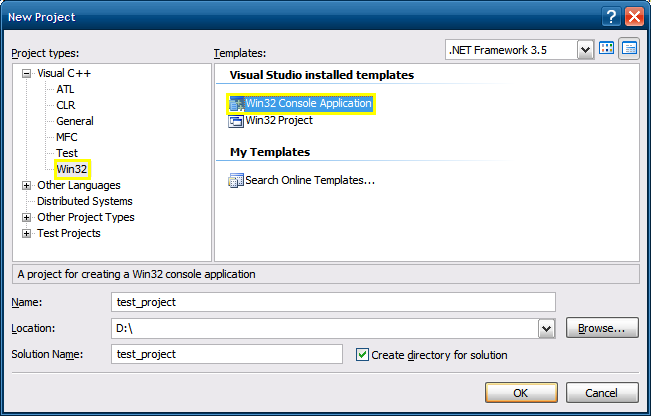
\includegraphics[scale=0.6]{1/Select_project_type}
  \end{figure}

Чтобы собрать проект, выберите пункт меню Build -> Build Solution
(Ctrl + Shift + B), затем выберите Debug -> Start Without Debugging
(Ctrl + F5) для запуска. Если хотите запустить под отладкой, то
выбирайте Debug -> Start Debugging (F5).

\section{Программа волнового поиска минимального пути}

\subsection{Описание алгоритма}

Алгоритм поиска одного из минимальных путей в неориентированном графе
является волновым и основан на понятии волны. В рамках этого алгоритма
волной называется множество вершин, каждая из которых является в
обрабатываемом графе смежной хотя бы одной вершине из предыдущей
волны. Волна, для которой нет предыдущей волны, называется начальной и
состоит из вершины, от которой начинается поиск минимального
пути. Волна, включающая конечную вершину пути, называется
конечной. Таким образом, наш алгоритм можно задать следующим перечнем
шагов:

\begin{enumerate}
\item Добавить все вершины графа, кроме начальной вершины пути, во
  множество непроверенных вершин.

\item Создать новую волну и добавить в нее начальную вершину пути.

\item Начальная волна – это новая волна. Новой волной будем называть
  последнюю созданную волну.

\item Сформировать следующую волну для новой волны. В нее попадет та
  вершина, которая является смежной вершине из новой волны и
  присутствует во множестве непроверенных вершин. Если вершина попала
  в формируемую волну, то ее надо исключить из множества непроверенных
  вершин. Созданную волну установить как следующую для новой волны, и
  после этого созданную волну считать новой волной.

\item Если новая волна пуста, то между вершинами не существует
  пути. Завершить алгоритм.

\item Если в текущей волне есть конечная вершина, то перейти к пункту
  7, иначе к пункту 4.

\item Сформировать один из минимальных путей, проходя в обратном
  порядке по списку волн. Завершить алгоритм.
\end{enumerate}

\subsection{Тестовые примеры}
\label{sec:Cppalgo_tests}

1.	graph1.txt

\begin{figure}[h!]
  \centering
  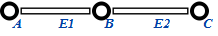
\includegraphics{1/test/1}
\end{figure}

2.	graph2.txt

\begin{figure}[h!]
  \centering
  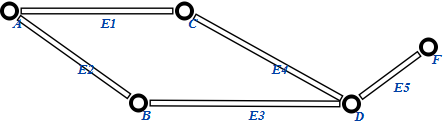
\includegraphics{1/test/2}
\end{figure}

3.	graph3.txt

\begin{figure}[h!]
  \centering
  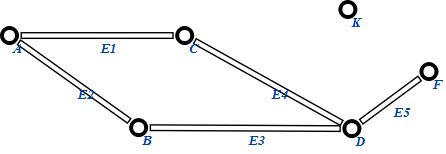
\includegraphics{1/test/3}
\end{figure}
 
4.	graph4.txt

\begin{figure}[h!]
  \centering
  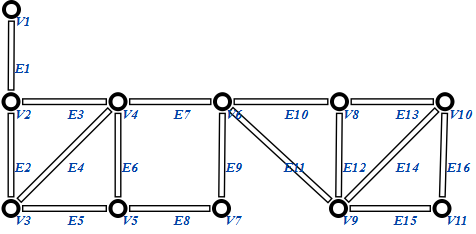
\includegraphics{1/test/4}
\end{figure}
 
5.	graph5.txt

\begin{figure}[h!]
  \centering
  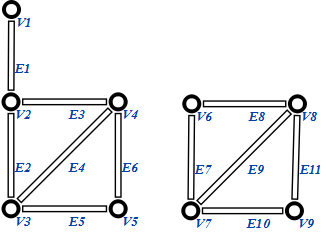
\includegraphics{1/test/5}
\end{figure}

\subsection{Создания программы}
\label{sec:Desc_prg}

%%% Local Variables: 
%%% mode: latex
%%% TeX-master: "main"
%%% End: 


\chapter{Построение фрагмента онтологии}
\label{cha:Onto}

Для понимания этого раздела студент должен обладать следующими
знаниями:

\begin{itemize}
\item базовые знания по теории графов
\item SC-коде и SC-алфавите
\item базовые знания о SCg-коде
\item уметь различать абсолютные и относительные понятия
\item знание правил формирования идентификаторов sc-элементов
\end{itemize}

\section{Задание}
\label{sec:Onto_task}

Во-первых, что должны сделать вы, студент, при выполнении
этого этапа расчетной работы, это выделить абсолютные и относительные
понятия своей теоретико-графовой задачи. Список понятий должен
включать не только непосредственно необходимые для решения вашей
задачи, но и те понятия, на основе которых определены непосредственно
необходимые. Таким образом, будет выделена целая иерархия понятий.

Во-вторых, для каждого понятия разработать способ представления его
экземпляров в SC-коде. Подготовить отчет в электронном варианте о
проделанной работе, который должен содержать следующее (пример отчета
приведен в разделе \ref{sec:Onto_example}):

\begin{enumerate}
\item перечень выделенных понятий со следующей информацией:
  \begin{enumerate}
  \item название понятия;
  \item абсолютное или относительное;
  \item определение на естественном языке (его стоит брать из соответствующей
    литературы);
  \item пример представления экземпляра понятия в SC-коде на
    SCg (не маленький и не большой, среднего размера). 
  \end{enumerate}
\item пять примеров на SCg входных и выходных данных для вашей
  программы (примеры нужно брать из предыдущего этапа расчетной
  работы и можно использовать сокращенную форму записи графов).
\end{enumerate}

Для рисования SCg-текстов необходимо использовать редактор KBE
(Knowledge Base Editor). Установщик и zip-архив собранной версии под
Windows можно найти в той же папке на сервере Info, откуда вы взяли
этот документ.

Мы плавно переходим к примеру выполнения 2-го этапа$\dots$

Выполненный мною пример отчета по этому этапу в docx-формате можно
найти в папке расчетной работы на сервере Info либо в конце этого
документа.  Напомню, что мы рассматриваем задачу поиска одного из
минимальных путей в неориентированном графе. Поэтому первым, чем мы
займемся, будет способ представления в SC-коде неориентированных и
ориентированных графов.


\section{Формализация понятий <<неориентированный>> и
  <<ориентированный граф>>}
\label{sec:Onto_form_undir_dir_graph}

Возьмем для рассмотрения неориентированный граф $G$:

\begin{figure}[h!]
  \centering
  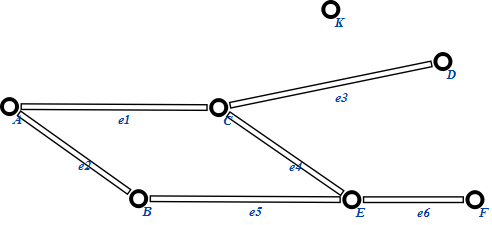
\includegraphics[scale=0.8]{2/Undirected_graph_not_scg}
  \caption{Неориентированный граф $G$ (это не SCg)}
  \label{fig:Undirected_graph_not_scg}
\end{figure}

Распишем граф $G$ классическим способом на языке теории множеств:

\begin{gather}
  G = \langle V_g,E_g \rangle; \label{eq:Graph_G_classical} \\
  V_g = \{A,B,C,E,D,F,K\}; \nonumber \\
  E_g = \{\{A,B\},\{A,C\},\{C,E\},\{C,D\},\{B,E\},\{E,F\}\}. \nonumber
\end{gather}

Теперь попробуем перевести запись, приведенную выше, в SC-код. Все
sc-конструкции я буду приводить на SCg. Для представления
неориентированного графа в SC-коде введем абсолютное понятие
\idtf{неориентированный граф} (в дальнейшем я буду использовать именно
такое форматирования для идентификаторов sc-элементов в
тексте). Теперь мы можем преобразовать запись на языке теории
множеств, задающую граф $G$, в SCg-конструкцию, которая изображена на
рис.~\ref{fig:Undirected_graph_Classical_method}.

\begin{figure}[h!]
  \centering
  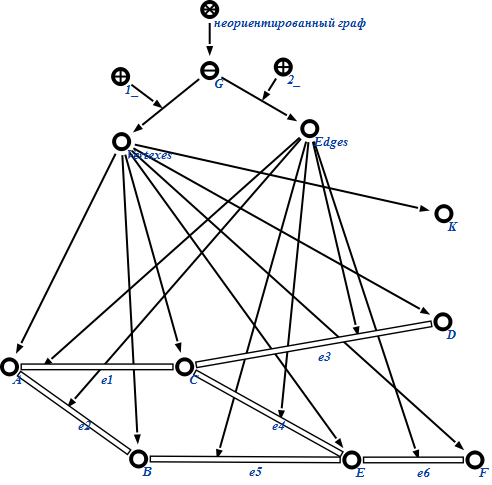
\includegraphics[scale=0.8]{2/Undirected_graph_Classical_method}
  \caption{Классический способ задания неориентированного графа $G$ на
    SCg}
  \label{fig:Undirected_graph_Classical_method}
\end{figure}

Приведенный выше способ задания графа на языке классической теории
множеств является распространённым, но мы, с использованием SC-кода,
можем найти другую форму, так как имеем возможность задавать ролевые
отношения. Поэтому введем два относительных понятия (ролевых
отношения): \idtf{вершина_} и \idtf{ребро_}. Тогда можно сформулировать,
что неориентированный граф задается множеством объектов, в котором
объект с ролью \idtf{вершина_} является вершиной графа, а объект с
ролью \idtf{ребро_} - ребром графа. На языке теории множеств,
расширенном возможностью задавать атрибуты (роли) у элементов кортежа,
граф G будет задаваться выражением~\eqref{eq:Graph_G_with_attrs}.

\begin{align}
  G &= \langle \idtf{вершина_}: A, \idtf{вершина_}: B, \idtf{вершина_}: C, \label{eq:Graph_G_with_attrs} \\
  & \idtf{вершина_}: E, \idtf{вершина_}: D, \idtf{вершина_}: F, \idtf{вершина_}: K, \nonumber \\
  & \idtf{ребро_}: \{A, B\}, \idtf{ребро_}: \{A, C\}, \idtf{ребро_}: \{C, E\}, \nonumber \\
  & \idtf{ребро_}: \{C, D\}, \idtf{ребро_}: \{B, E\},
  \idtf{ребро_}: \{E, F\} \rangle. \nonumber
\end{align}

Переведем выражение~\eqref{eq:Graph_G_with_attrs} в SCg, что показано
на рис.~\ref{fig:Undirected_graph_Main_method}.

\begin{figure}[h!]
  \centering
  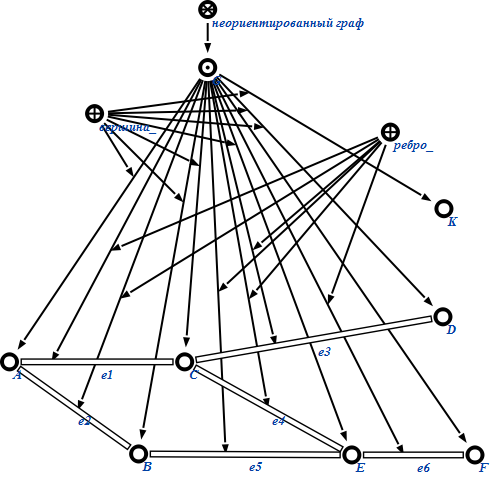
\includegraphics[scale=0.8]{2/Undirected_graph_Main_method}
  \caption{Основной для нас способ задания графа $G$ на SCg}
  \label{fig:Undirected_graph_Main_method}
\end{figure}

Для студента, знакомого с теорией множеств и SCg-языком, в
рис.~\ref{fig:Undirected_graph_Main_method} необходимо пояснить только
тип узла с идентификатором \idtf{G}. Такой тип SCg-узла используется
для обозначения sc-структуры, т.е. множества объектов, которые могут
выступать как целое. Объекты, которые входят в sc-структуру, при
совместном рассмотрении порождают некоторое новое качество. Попробуем
изучить это через сравнение множества \idtf{неориентированный граф} с
множеством \idtf{G}, которое является конкретным неориентированным
графом.

Множество \idtf{неориентированный граф} – является sc-понятием (к
слову, абсолютным), т.е. sc-множеством, все элементы которого обладают
некоторым заданным свойством. В случае sc-понятия
\idtf{неориентированный граф} его элементы должны обозначать
неориентированные графы. Предположим, в множестве
\idtf{неориентированный граф} у нас есть 5 элементов
(неориентированных графов). Добавим в это множество еще 5
неориентированных графов. При добавлении элементов мощность множества
изменилась, но качественно множество \idtf{неориентированный граф}
осталось таким же. Этот факт лаконично можно выразить следующим
образом: количество элементов множества, которое является sc-понятием,
никогда не переходит в качество.

Совсем по-другому обстоят дела с множеством \idtf{G}. Это
sc-множество, составлено из sc-элементов, которые вместе обладают
некоторой целостностью, имеющей важные свойства (они образуют
неориентированный граф только в том случае, если рассмотрены как
единое целое). Если мы добавим в множество \idtf{G} новый
элемент (вершину или ребро), то получим уже другой граф. Таким образом,
можно заключить, что количество элементов для множество \idtf{G}
переходит в качество. Множества, для которых выполняется это свойство,
являются sc-структурами.

Продолжая разговор о структурах, стоит сказать, что связки так же
являются структурами. Однако, очевидно, что неориентированный граф
\idtf{G} не только обозначает сам факт существования связи между
объектами, но и включает связки между своими собственными
элементами. Такие структуры, как граф \idtf{G} не являются связками, и
мы будем называть их одноуровневыми реляционными структурами.  Способ
представления графов в виде одноуровневых реляционных структур
используется в проекте базы знаний по теории графов технологии OSTIS
(\ostisgtlink), поэтому
ниже рассматривается только этот способ, и при выполнении расчетной
работы должен использоваться только он.

Продолжим рассмотрение того, как кодировать графы на sc-языках.
Давайте попробуем представить ориентированный граф на SCg. Преобразуем
неориентированный граф $G$ в ориентированный граф $G_d$
(рис.~\ref{fig:Directed_graph_not_scg}).

\begin{figure}[h!]
  \centering
  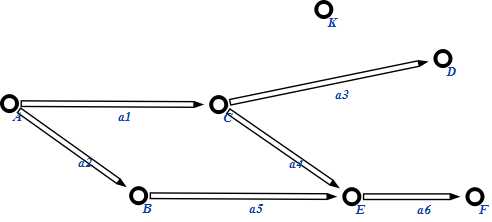
\includegraphics[scale=0.8]{2/Directed_graph_not_scg}
  \caption{Ориентированный граф $G_d$ (это не SCg)}
  \label{fig:Directed_graph_not_scg}
\end{figure}

Для представления $G_d$ на SCg введем абсолютное понятие
\idtf{ориентированный граф} и относительное понятие (ролевое
отношение) \idtf{дуга_}. С использованием этих понятий граф $G_d$ на
SCg можно представить так, как показано на
рис.~\ref{fig:Directed_graph}.

\begin{figure}[h]
  \centering
  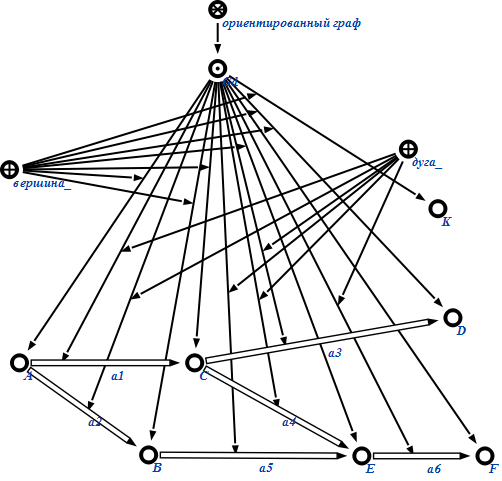
\includegraphics[scale=0.8]{2/Directed_graph}
  \caption{Ориентированный граф $G_d$ в SCg}
  \label{fig:Directed_graph}
\end{figure}

Сравните запись графа \idtf{G}
(рис.~\ref{fig:Undirected_graph_Main_method}) на SCg и графа
\idtfm{$G_d$} (рис.~\ref{fig:Directed_graph}). Разница только в
использовании:

\begin{itemize}
\item узла \idtf{ориентированный граф} вместо \idtf{неориентированный
    граф};
\item узла \idtf{дуга_} вместо \idtf{ребро_};
\item \underline{ориентированных} бинарных пар вместо
  неориентированных.
\end{itemize}

Можно заметить, что графы на SCg с использованием ролевых отношений
\idtf{вершина_} и \idtf{ребро_} получаются очень громоздкими, поэтому в
дальнейших объяснениях для представления неориентированных и
ориентированных графов мы будем использовать сокращенную запись. С
использованием сокращенной записи граф \idtf{G}, заданный на
рис.~\ref{fig:Undirected_graph_Main_method}, мы будем задавать так,
как показано на рис.~\ref{fig:Undirected_graph_Short_form}. Надеюсь:
читатель понимает, что эта запись предназначена для восприятия
человеком, а не машиной, потому что для машины является важным наличие
опущенных атрибутов.

\begin{figure}[h!]
  \centering
  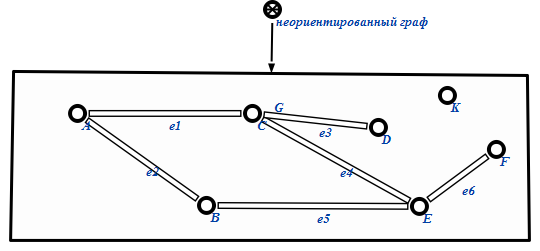
\includegraphics[scale=0.8]{2/Undirected_graph_Short_form}
  \caption{Сокращенная форма задbания графа $G$ на SCg Мы определились,}
  \label{fig:Undirected_graph_Short_form}
\end{figure}

Мы рассмотрели способ формализации с использованием семантических
сетей неориентированных и ориентированных графов. Теперь перейдем к
формализации минимального пути - второго понятия, без которого не
обойтись при решении нашей задачи.

\section{Формализация понятия <<минимальный путь>>}
\label{sec:Onto_form_min_path}

Если читатель заглянет в книгу Харарри <<Теория графов>> на страницу
26, то в начале главы <<Маршруты и связность>> он может прочитать
следующее:

\begin{quotation}
  \textbf{Маршрутом} в графе $G$ называется чередующаяся
  последовательность вершин и ребер $v_0$, $x_1$, $v_1$, $\dotsc$,
  $v_{n-1}$, $x_n$, $v_n$; эта последовательность начинается и
  кончается вершиной, и каждое ребро последовательности инцидентно
  двум вершинам, одна из которых непосредственно предшествует ему, а
  другая непосредственно следует за ним. Указанный маршрут соединяет
  вершины $v_0$ и $v_n$, и его можно обозначить $v_0$, $v_1$,
  $\dotsc$, $v_n$ (наличие ребер подразумевается). $\dots$ Маршрут
  называется \textbf{цепью}, если все его ребра различны, и
  \textbf{простой цепью} (\textbf{путем}), если все вершины (а,
  следовательно, и ребра) различны.
\end{quotation}

Таким образом, путь — это маршрут, поэтому сейчас мы будем
рассматривать именно это более общее понятие. Если разберемся с
представлением его в SC-коде, то разберемся и с более частным
понятием.

Я думаю, что для читателя очевидно следующее: маршрут – это
относительное понятие, так как конкретный маршрут существует в связи с
конкретным графом. Поэтому для представления маршрутов введем бинарное
ориентированное отношение \idtf{маршрут*}. Первым компонентом связки
этого отношения будет знак графа, а вторым знак структуры
маршрута. Пример связки приведен на
рис.~\ref{fig:Example_of_relations_Route_tuple}.

\begin{figure}[h]
  \centering
  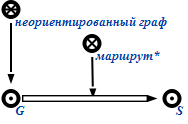
\includegraphics{2/Example_of_relations_Route_tuple}
  \caption{Пример связки отношения \idtf{маршрут*}}
  \label{fig:Example_of_relations_Route_tuple}
\end{figure}

Теперь нам необходимо выяснить из чего же состоит структура \idtf{S}
на рис.~\ref{fig:Example_of_relations_Route_tuple}. Для этого
рассмотрим в графе \idtf{G}
(рис.~\ref{fig:Undirected_graph_Short_form}) маршрут \idtf{R} между
вершинами \idtf{A} и \idtf{F}, который задается последовательностью
\idtf{A}, \idtfm{$e_2$}, \idtf{B}, \idtfm{$e_5$}, \idtf{E},
\idtfm{$e_6$}, \idtf{F} (это один из минимальных путей между \idtf{A} и
\idtf{F}). Если маршрут состоит из вершин и ребер, то его можно
представить как подграф графа, на котором задается маршрут. Посмотрите
внимательно на риc.~\ref{fig:Route_as_subgraph}.

\begin{figure}
  \centering
  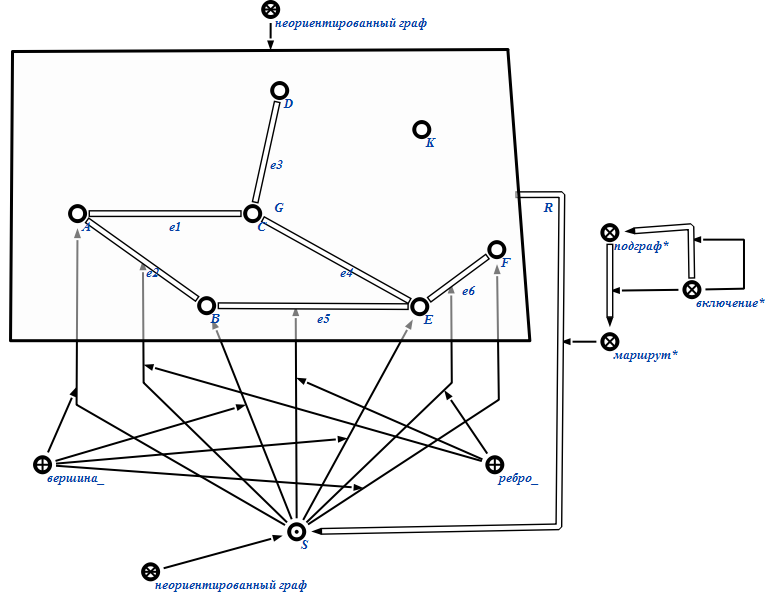
\includegraphics[scale=0.8]{2/Route_as_subgraph}
  \caption{Представление маршрута как подграфа графа \idtf{G}}
  \label{fig:Route_as_subgraph}
\end{figure}

Наверное, вы обратили внимание, что на
рис.~\ref{fig:Route_as_subgraph} появилось бинарное ориентированное
отношение \idtf{подграф*}, суть которого есть связывание одного графа
с другим графом, который является подграфом первого. А еще из
рис.~\ref{fig:Route_as_subgraph} вы можете заметить, что отношение
\idtf{включение*} включает отношение \idtf{подграф*},
т.е. \idtf{подграф*} - аналог \idtf{включения*}, но только для
графов. А наше отношение \idtf{маршрут*} является подмножеством
отношения \idtf{подграф*}. Таким образом, граф структуры \idtf{S}
является подграфом исходного графа \idtf{G}.

Возможно, вы посчитали, что на этом наш разговор о способе
представления маршрутов можно закончить, но я попрошу вас не
торопиться, а попробовать нарисовать SCg-конструкцию, которая задаст
маршрут \idtf{A}, \idtfm{$e_2$}, \idtf{B}, \idtfm{$e_5$}, \idtf{E},
\idtfm{$e_4$}, \idtf{С}, \idtfm{$e_1$}, \idtf{A}, \idtfm{$e_2$},
\idtf{B}. Ну как? Получилось? Хоть это и не путь, потому что вершины и
ребра повторяются, но это вполне допустимый маршрут. А все из-за
повторяющихся вершин и ребер. На
рис.~\ref{fig:Route_as_subgraph_problem} повторяющиеся вершины и ребра
выделены красным цветом. Поэтому мы опять переходим к поиску способа
задать структуру второго компонента связки отношения \idtf{маршрут*}
(структура \idtf{S} на
рисунке~\ref{fig:Example_of_relations_Route_tuple}).

\begin{figure}
  \centering
  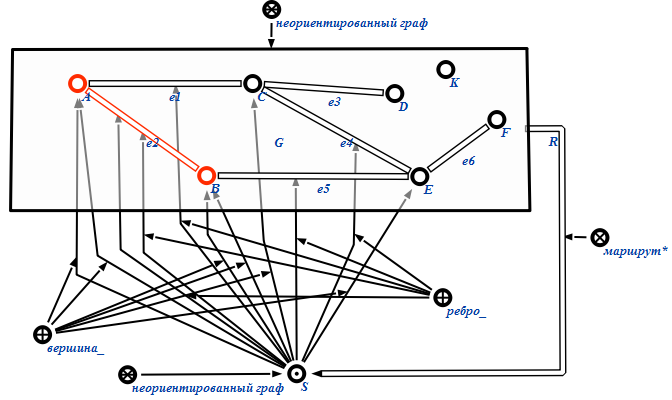
\includegraphics[scale=0.8]{2/Route_as_subgraph_problem}
  \caption{Проблема представления маршрута как подграфа графа \idtf{G}}
  \label{fig:Route_as_subgraph_problem}
\end{figure}

Вернемся к тому, что мы решили рассматривать маршрут \idtf{R} в графе
\idtf{G}. Тогда в основу нашего способа представления мы положили, что
маршрут состоит из вершин и ребер и он есть подграф графа, на котором
задается. Может быть, слабость этого подхода была в том, что мы не
рассматривали маршрут как последовательность вершин и ребер, т.е. мы
не задали порядок? Давайте попробуем задать последовательность
элементов маршрута.

Как мы можем задать последовательность? Если без введения лишних
понятий, то, например, при помощи ориентированного графа. Вершинами
такого графа будут элементы последовательности, а дуги будут задавать
отношение предыдущий/следующий. Первый элемент последовательности
специально указывать не будем, потому что первым элементом является
вершина, в которую нет входящих дуг. Последним элементом
последовательности будет вершина, из которой нет исходящих дуг. Этот
способ представления маршрута \idtf{R} показан на
рис.~\ref{fig:Route_as_sequence} (\textcolor{blue}{синим цветом}
выделены элементы маршрута, а \textcolor{green}{зеленым} - связки
следующий/предыдущий).

\begin{figure}
  \centering
  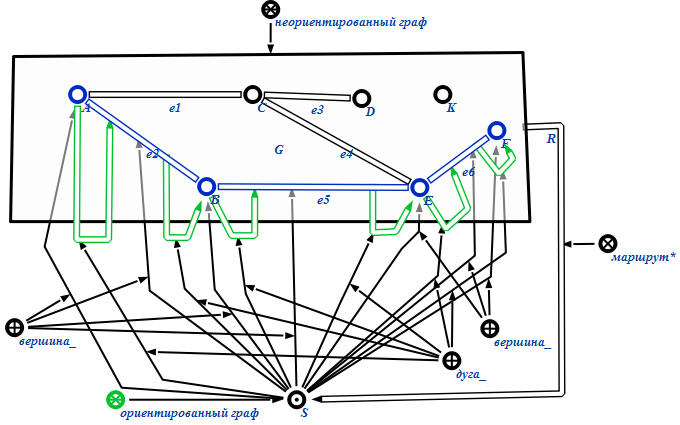
\includegraphics[scale=0.8]{2/Route_as_sequence}
  \caption{Представление маршрута через ориентированный граф последовательности}
  \label{fig:Route_as_sequence}
\end{figure}

Но, даже используя новый способ представления, мы не сможем задать
маршрут, который не является цепью или простой цепью (путем). Новый
способ представления все равно ограничен. Предлагаю вам увидеть это
самостоятельно, представив маршрут с повторяющимися вершинами и
ребрами. Поэтому продолжим наш поиск.

Давайте еще раз взглянем на определение маршрута из <<Теории графов>>:

\begin{quotation}
  \textbf{Маршрутом} в графе $G$ называется чередующаяся
  последовательность вершин и ребер $v_0$, $x_1$, $v_1$, $\dotsc$, $v_{n-1}$,
  $x_n$, $v_n$;
\end{quotation}

В нем сказано, что маршрут состоит из вершин и ребер. Но, быть может,
это не совсем так? Мы нашли два ограниченных способа для представления
маршрута, пользуясь буквально этим определением, а задачу еще не
решили. Может быть, стоит сказать, что маршрут состоит не из
последовательности вершин и ребер, а из последовательности посещений
вершин и ребер. Давайте попробуем использовать именно такую точку
зрения. Тогда мы можем преобразовать ориентированный граф
последовательности \idtf{S} из рис.~\ref{fig:Route_as_sequence} в
ориентированный граф посещений \idtf{S} на
рис.~\ref{fig:Route_as_correspondence_Incomplete}. Вершина графа
\idtf{S} на рис.~\ref{fig:Route_as_correspondence_Incomplete}
обозначает посещение вершины графа \idtf{G}, а дуга графа \idtf{S} –
посещение ребра графа \idtf{G}.

\begin{figure}[h!]
  \centering
  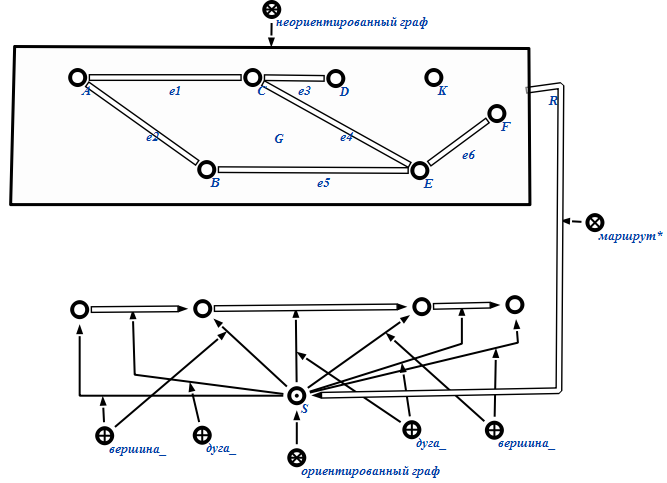
\includegraphics[scale=0.8]{2/Route_as_correspondence_Incomplete}
  \caption{Представление структуры \idtf{S} маршрута \idtf{R} как
    ориентированного графа посещений}
  \label{fig:Route_as_correspondence_Incomplete}
\end{figure}

На рис.~\ref{fig:Route_as_correspondence_Incomplete} не хватает только
связей между элементами посещения из графа $S$ и посещенными
элементами из графа $G$. Для того, чтобы мы могли закончить
конструкцию рис.~\ref{fig:Route_as_correspondence_Incomplete}, вам
надо вспомнить, что такое соответствие между двумя множествами, а,
если вы этого не знаете, то устранить пробел в вашем образовании. А
тем временем мы введем относительное понятие (тернарное отношение)
\idtf{соответствие*}, связка которого включает следующие три
компонента (пример связки на
рис.~\ref{fig:Relation_Correspondence_example}):

\begin{enumerate}
\item множество, которое является областью определения соответствия
  (множество \idtf{X}).
\item множество, которое является областью значений соответствия
  (множество \idtf{Y}).
\item бинарное ориентированное отношение, которое устанавливает
  соответствие между элементом из области определения и элементом из
  области значения (отношение \idtf{Cr*}).
\end{enumerate}

\begin{figure}[h!]
  \centering
  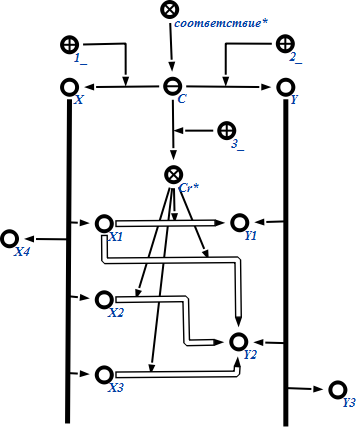
\includegraphics[scale=0.8]{2/Relation_Correspondence_example}
  \caption{Пример связки C отношения \idtf{соответствие*} между
    множествами $X$ и $Y$}
  \label{fig:Relation_Correspondence_example}
\end{figure}

Мы можем рассматривать маршрут \idtf{R} как всюду определенное,
функциональное соответствие между ориентированным графом (структурой
маршрута) \idtf{S} и неориентированным исходным графом \idtf{G}.
Тогда на основе
рис.~\ref{fig:Route_as_correspondence_Incomplete}~и~\ref{fig:Relation_Correspondence_example}
построим окончательный вариант представления маршрута \idtf{R}
(рис.~\ref{fig:Route_as_correspondence_Final}). Рассмотрим отличия
рис.~\ref{fig:Route_as_correspondence_Final} от
рис.~\ref{fig:Route_as_correspondence_Incomplete}:

\begin{enumerate}
\item Для наглядности упрощен ориентированный граф \idtf{S} (скрыты
  узлы \idtf{вершина_} и \idtf{дуга_}).
\item Показано, что отношение \idtf{маршрут*} является подмножеством
  отношения \idtf{соответствие*}.
\item В связке \idtf{R} первым компонентом теперь является граф
  \idtf{S}, а вторым – граф \idtf{G}. На
  рис.~\ref{fig:Route_as_correspondence_Incomplete} было
  наоборот. Чтобы понять, почему связка оказалась перевернутой,
  взгляните, пожалуйста, на
  рис.~\ref{fig:Relation_Correspondence_example}. На нем видно, что
  первым компонентом связки отношения \idtf{соответствие*} должно быть
  множество, которое является областью определения, а вторым –
  множество, которое является областью значения. Именно поэтому
  произошла такая перестановка.
\item Появилось отношения (третий компонент связки \idtf{R}), которое
  задает соответствие между посещением и посещенным
  элементом. \underline{Обратите внимание} на направление бинарных
  ориентированных пар этого отношения!
\end{enumerate}

\begin{figure}[h!]
  \centering
  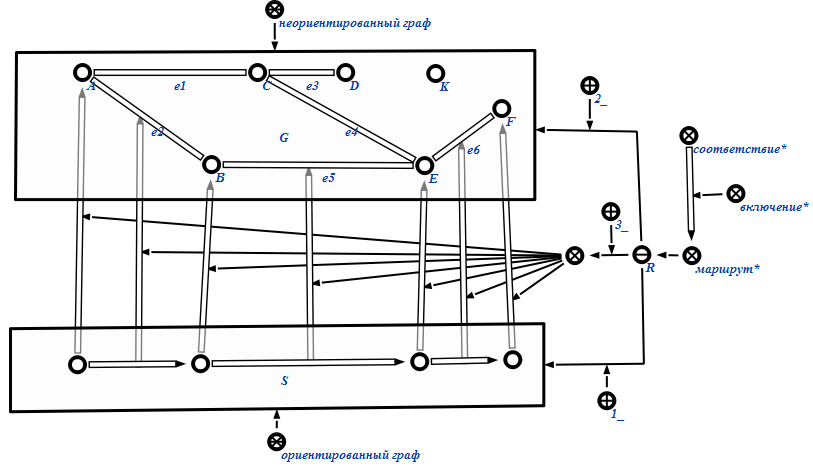
\includegraphics[scale=0.6]{2/Route_as_correspondence_Final}
  \caption{Окончательный вариант представления маршрута \idtf{R}, как
    соответствия между графом \idtf{S} и графом \idtf{G}}
  \label{fig:Route_as_correspondence_Final}
\end{figure}

Попробуйте представить при помощи найденного нами способа
(рис.~\ref{fig:Route_as_correspondence_Final}) маршрут, в котором есть
повторяющиеся вершина и/или ребра. Я думаю, что теперь с этим у вас не
возникнет проблем. Подводя к концу разговор о способе представления
маршрутов в графе, введем относительные понятия (бинарные
ориентированные отношения) \idtf{цепь*} и \idtf{путь*}, которые
связаны с отношением \idtf{маршрут*} так, как показано на
рис.~\ref{fig:Relations_Trail_and_Path}.

\begin{figure}[h!]
  \centering
  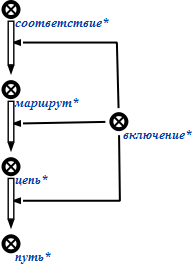
\includegraphics[scale=0.8]{2/Relations_Trail_and_Path}
  \caption{Связь отношений \idtf{цепь*} и \idtf{путь*} с отношением
    \idtf{маршрут*}}
  \label{fig:Relations_Trail_and_Path}
\end{figure}

Тогда один из минимальных путей \idtf{R} (\idtf{A}, \idtfm{$e_2$},
\idtf{B}, \idtfm{$e_5$}, \idtf{E}, \idtfm{$e_6$}, \idtf{F}) в графе
\idtf{G} между вершинами \idtf{A} и \idtf{F} будет представляться в
SC-коде так, как показано на рис.~\ref{fig:Path_Final}. Правда,
несильно отличается от рис.~\ref{fig:Route_as_correspondence_Final}?

\begin{figure}[h!]
  \centering
  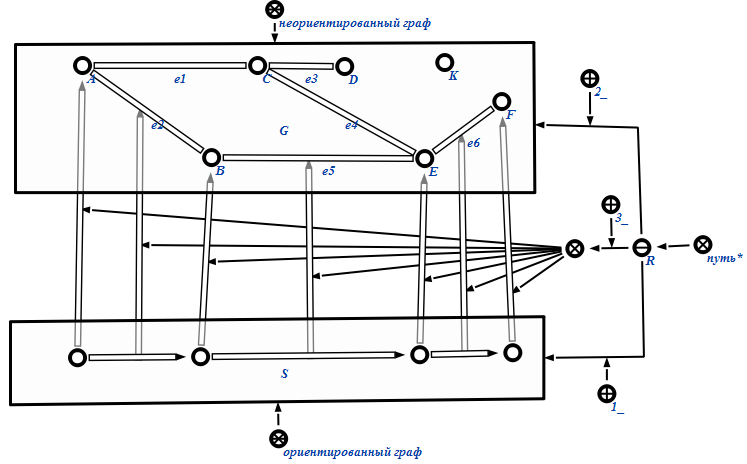
\includegraphics[scale=0.6]{2/Path_Final}
  \caption{Один из минимальных путей \idtf{R} между вершинами \idtf{А}
    и \idtf{F} графа \idtf{G}}
  \label{fig:Path_Final}
\end{figure}

На этом мы заканчиваем разговор о минимальном пути и переходим к
разговору о том, как можно обобщить представление различных видов
графов в SC-коде.

\section{Обобщение различных видов графов с использованием понятия
  графовой структуры}
\label{sec:Onto_graph_struct}

В предыдущем разделе, когда мы искали способ представления
минимального пути в SC-коде, то сосредоточились на представлении
наиболее общего понятия по отношению к понятию путь, а именно –
маршрута. Таким образом, определившись с кодированием понятия
\idtf{маршрут*}, мы определились и с кодированием понятия
\idtf{путь*}. А вот, когда мы разбирались с неориентированными и
ориентированными графами, то рассматривали только то, что необходимо
для решения нашей задачи, игнорируя более общие случаи. Теперь пришло
время посмотреть на задачу представления графов в SC-коде более
широко. Для этого мы обратимся к базе знаний по теории графов из
проекта \ostisgtlink. Неполная иерархия различных типов графов из этой
базы знаний изображена на рис.~\ref{fig:Hierarchy_of_graphs_types}. Я
думаю, что вы уже заметили узлы ориентированный граф и
неориентированный граф. Однако они составляют только <<низ>> иерархии,
так как определены на основе более общих понятий. А начнем
рассматривать иерархию с <<верха>>, а именно, с понятия \idtf{графовая
  структура}.

\begin{figure}[h!]
  \centering
  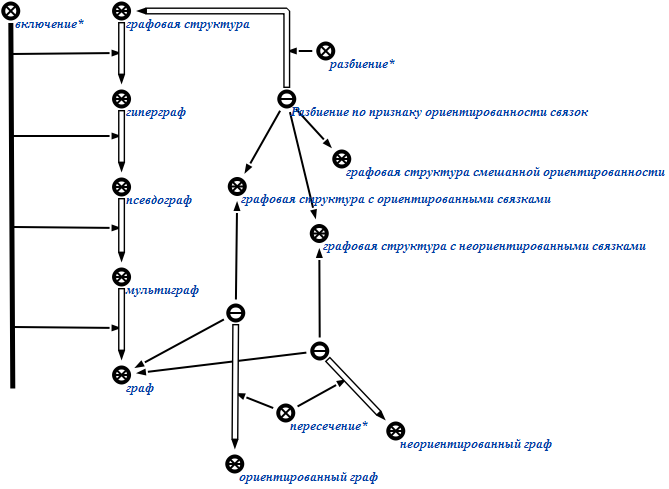
\includegraphics[scale=0.95]{2/Hierarchy_of_graphs_types}
  \caption{Иерархия различных типов графовых структур (Это неполная
    иерархия из \ostisgtlink)}
  \label{fig:Hierarchy_of_graphs_types}
\end{figure}

Экземпляр понятия \idtf{графовая структура} – это такая одноуровневая
реляционная структура, которая содержит объекты с ролью
\idtf{вершина_}, а связки между этими объектами - с ролью
\idtf{связка_}. Вроде бы по определению \idtf{графовая структура}
несильно отличается от \idtf{неориентированного графа}. Взяли просто и
заменили ролевое отношение \idtf{ребро_} на \idtf{связка_}. И вот тут
есть один нюанс. На элементы с ролью \idtf{связка_} \idtf{графовой
  структуры} не накладывается ограничений, как на элементы с ролью
\idtf{ребро_} \idtf{неориентированного графа}, а именно:

\begin{itemize}
\item они могут быть любой арности, а не только бинарными;
\item они могут быть как ориентированными, так и неориентированными;
\item их компонентами могут быть не только вершины, но и другие связки
  (т.е. разрешены связки, <<выходящие>> из связок, и связки, входящие
  в другие связки).
\end{itemize}

На рис.~\ref{fig:Graph_structure_example} приведен пример графовой
структуры \idtfm{$G_s$}, в которой четыре вершины и три связки. Я хочу
отметить, что графовая структура вполне может включать элементы с
ролью \idtf{ребро_}. Просто \idtf{связка_} более общее понятие, чем
\idtf{ребро_}. Чтобы лучше увидеть связь между этими ролевыми
отношениями, рассмотрите
рис.~\ref{fig:Hierarchy_of_elements_roles_in_graph_structure}, на
котором изображена иерархия ролевых отношений элементов графовой
структуры из базы знаний по теории графов. А после того, как
закончите, мы перейдем к краткому описанию абсолютных понятий
\idtf{гиперграф}, \idtf{псевдограф}, \idtf{мультиграф} и \idtf{граф}.

\begin{figure}[h!]
  \centering
  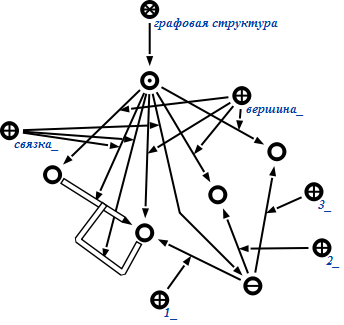
\includegraphics{2/concept/Graph_structure}
  \caption{Пример графовой структуры \idtfm{$G_s$}}
  \label{fig:Graph_structure_example}
\end{figure}
 
\begin{figure}[h!]
  \centering
  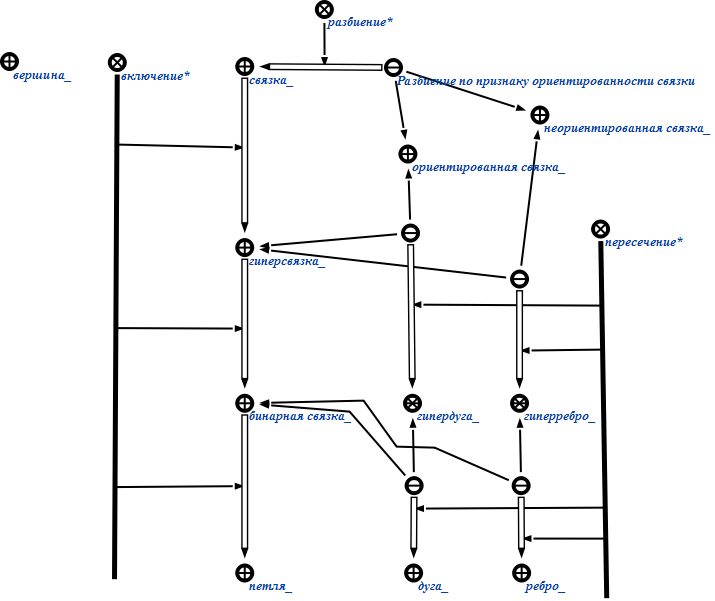
\includegraphics[scale=0.95]{2/Hierarchy_of_elements_roles_in_graph_structure}
  \caption{Иерархия ролей элементов графовой структуры (Это неполная
    иерархия из \ostisgtlink)}
  \label{fig:Hierarchy_of_elements_roles_in_graph_structure}
\end{figure}

Экземпляр понятия \idtf{гиперграф}
(см. рис.~\ref{fig:Hierarchy_of_graphs_types}) – это такая графовая
структура, в которой элемент с ролью \idtf{связка_} может иметь в
качестве своих компонентов только элемент с ролью \idtf{вершина_} этой
графовой структуры.  На арность связок никакого ограничения не
накладывается. Для указания связки введены ролевые отношения
\idtf{гиперсвязка_}, \idtf{гипердуга_}, \idtf{гиперребро_}
(рис.~\ref{fig:Hierarchy_of_elements_roles_in_graph_structure}). Обратите
внимание на то, что на
рис.~\ref{fig:Hierarchy_of_elements_roles_in_graph_structure}
\idtf{гипердуга_} определена как пересечение понятий \idtf{гиперсвязка_}
и {ориентированная связка}. Аналогично дела обстоят с понятием
\idtf{гиперребро_}. Пожалуйста, обдумайте самостоятельно такой способ
введения новых понятий.

Экземпляр понятия \idtf{псевдограф}
(см. рис.~\ref{fig:Hierarchy_of_graphs_types}) – это такой гиперграф,
в котором гиперсвязка может иметь только два компонента.  Для указания
связки введены ролевые отношения \idtf{бинарная связка_}, \idtf{петля_},
\idtf{дуга_}, \idtf{ребро_}
(рис.~\ref{fig:Hierarchy_of_elements_roles_in_graph_structure}). Петлей
называется бинарная связка, у которой оба компонента одинаковы.

Экземпляр понятия \idtf{мультиграф}
(см. рис.~\ref{fig:Hierarchy_of_graphs_types}) – это такой псевдограф,
в котором не может быть петель.
 
Экземпляр понятия \idtf{граф}
(см. рис.~\ref{fig:Hierarchy_of_graphs_types}) – это такой мультиграф,
в котором не может быть кратных связок, т.е. связок у которых первый и
второй компоненты совпадают.

А теперь самостоятельно на основе
рис.~\ref{fig:Hierarchy_of_graphs_types} рассмотрите то, как
определены уже знакомые вам понятия \idtf{ориентированный граф} и
\idtf{неориентированный граф}. 

\newpage

\section{Пример выполнения}
\label{sec:Onto_example}

\subsection{Список понятий}
\label{sec:Onto_ex_concepts}

\begin{itemize}
\item Графовая структура (абсолютное понятие) - это такая
  одноуровневая реляционная структура, объекты которой могут играть
  роль либо вершины, либо связки:
  \begin{itemize}
  \item Вершина (относительное понятие, ролевое отношение);
  \item Связка (относительное понятие, ролевое отношение).
  \end{itemize}

  \begin{figure}[h!]
    \centering
    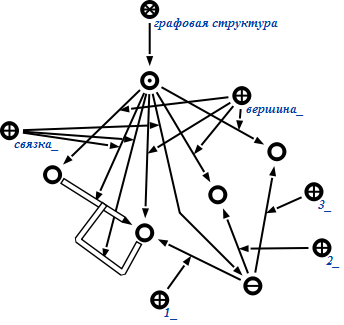
\includegraphics[scale=0.8]{2/concept/Graph_structure}
    \label{fig:Concept_Graph_structure}
  \end{figure}

\newpage

\item Графовая структура с ориентированными связками (абсолютное
  понятие)
  \begin{itemize}
  \item Ориентированная связка (относительное понятие, ролевое
    отношение) – связка, которая задается ориентированным множеством.
  \end{itemize}

  \begin{figure}[h!]
    \centering
    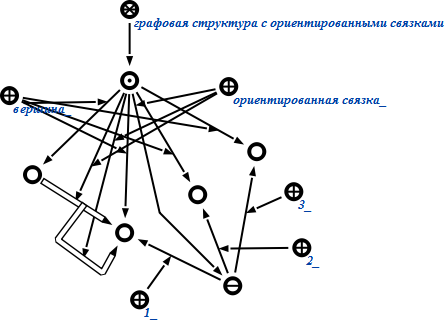
\includegraphics[scale=0.8]{2/concept/Directed_graph_structure}
    \label{fig:Concept_Directed_graph_structure}
  \end{figure}

\newpage

\item Графовая структура с неориентированными связками (абсолютное
  понятие)
  \begin{itemize}
  \item Неориентированная связка (относительное понятие, ролевое
    отношение) – связка, которая задается неориентированным
    множеством.
  \end{itemize}

  \begin{figure}[h!]
    \centering
    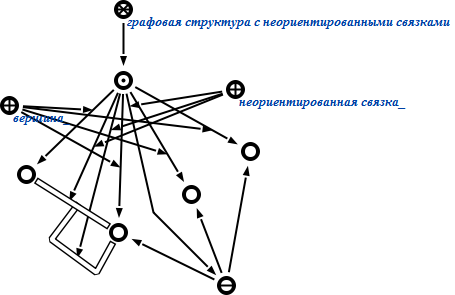
\includegraphics[scale=0.8]{2/concept/Undirected_graph_structure}
    \label{fig:Concept_Undirected_graph_structure}
  \end{figure}

\newpage

\item Гиперграф (абсолютное понятие) – это такая графовая структура, в
  которой связки могут связывать только вершины:
  \begin{itemize}
  \item Гиперсвязка (относительное понятие, ролевое отношение);
  \item Гипердуга (относительное понятие, ролевое отношение) –
    ориентированная гиперсвязка;
  \item Гиперребро (относительное понятие, ролевое отношение) –
    неориентированная гиперсвязка.
  \end{itemize}

  \begin{figure}[h!]
    \centering
    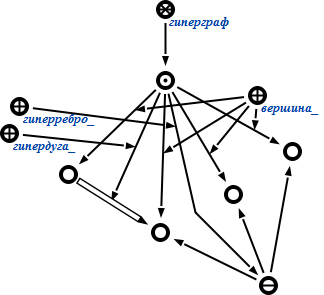
\includegraphics[scale=0.8]{2/concept/Hypergraph}
    \label{fig:Concept_Hypergraph}
  \end{figure}

\newpage

\item Псевдограф (абсолютное понятие) – это такой гиперграф, в котором
  все связки должны быть бинарными.
  \begin{itemize}
  \item Бинарная связка (относительное понятие, ролевое отношение)
    – гиперсвязка арности 2; 
  \item Ребро (относительное понятие, ролевое
    отношение) – неориентированная гиперсвязка;
  \item Дуга (относительное понятие, ролевое отношение) –
    ориентированная гиперсвязка;
  \item Петля (относительное понятие, ролевое отношение) – бинарная
    связка, у которой первый и второй компоненты совпадают.
  \end{itemize}

  \begin{figure}[h!]
    \centering
    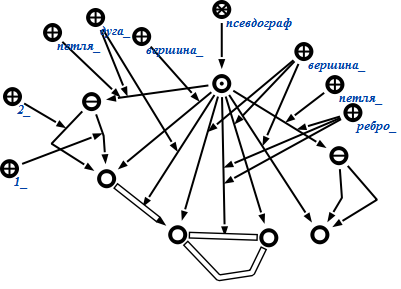
\includegraphics[scale=0.8]{2/concept/Pseudograph}
    \label{fig:Concept_Pseudograph}
  \end{figure}

\newpage

\item Мультиграф (абсолютное понятие) – это такой псевдограф, в
  котором не может быть петель.

  \begin{figure}[h!]
    \centering
    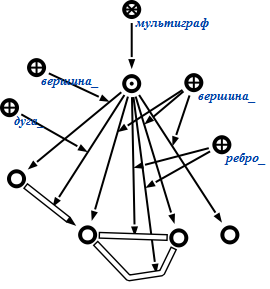
\includegraphics[scale=0.8]{2/concept/Multigraph}
    \label{fig:Concept_Multigraph}
  \end{figure}

\newpage
 
\item Граф (абсолютное понятие) – это такой мультиграф, в котором не
  может быть кратных связок, т.е. связок у которых первый и второй
  компоненты совпадают.

  \begin{figure}[h!]
    \centering
    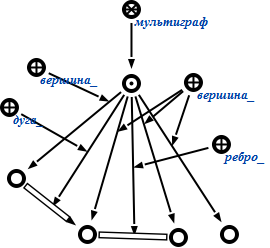
\includegraphics[scale=0.8]{2/concept/Graph}
    \label{fig:Concept_Graph}
  \end{figure}

\newpage
 
\item Неориентированный граф (абсолютное понятие) – это такой граф, в
  котором все связки являются ребрами:

  \begin{figure}[h!]
    \centering
    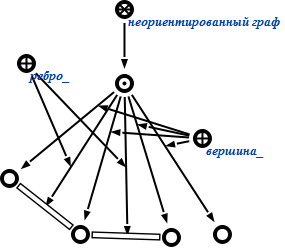
\includegraphics[scale=0.8]{2/concept/Undirected_graph}
    \label{fig:Concept_Undirected_graph}
  \end{figure}

\newpage
 
\item Ориентированный граф (абсолютное понятие) - это такой граф, в
  котором все связки являются дугами:

  \begin{figure}[h!]
    \centering
    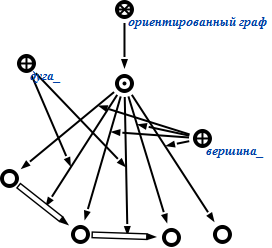
\includegraphics[scale=0.8]{2/concept/Directed_graph}
    \label{fig:Concept_Directed_graph}
  \end{figure}

\newpage
 
\item Маршрут (относительное понятие, бинарное ориентированное
  отношение) – это чередующаяся последовательность вершин и
  гиперсвязок в гиперграфе, которая начинается и кончается вершиной, и
  каждая гиперсвязка последовательности инцидентна двум вершинам, одна
  из которых непосредственно предшествует ей, а другая непосредственно
  следует за ней. В примере ниже показан маршрут \idtf{A},
  \idtf{CON1}, \idtf{C}, \idtf{CON2}, \idtf{D}, \idtf{CON3}, \idtf{B},
  \idtf{CON1}, \idtf{A} в гиперграфе. Обратите внимание, что графы в
  примере приведены в сокращенной форме, что \idtf{CON1} – это
  тернарная неориентированная связка (гиперсвязка), а \idtf{CON2} и
  \idtf{CON3} – бинарные связки (гиперсвязки).

  \begin{figure}[h!]
    \centering
    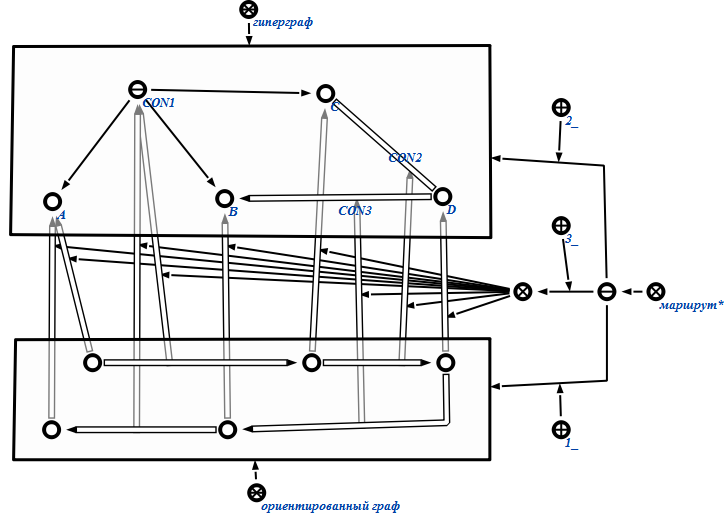
\includegraphics[scale=0.8]{2/concept/Route}
    \label{fig:Concept_Route}
  \end{figure}

\newpage
 
\item Цепь (относительное понятие, бинарное ориентированное отношение)
  – это маршрут, все гиперсвязки которого различны. В примере ниже
  показана цепь \idtf{A}, \idtf{CON1}, \idtf{C}, \idtf{CON2},
  \idtf{D}, \idtf{CON3}, \idtf{B}, \idtf{CON1}, \idtf{A} в гиперграфе.

  \begin{figure}[h!]
    \centering
    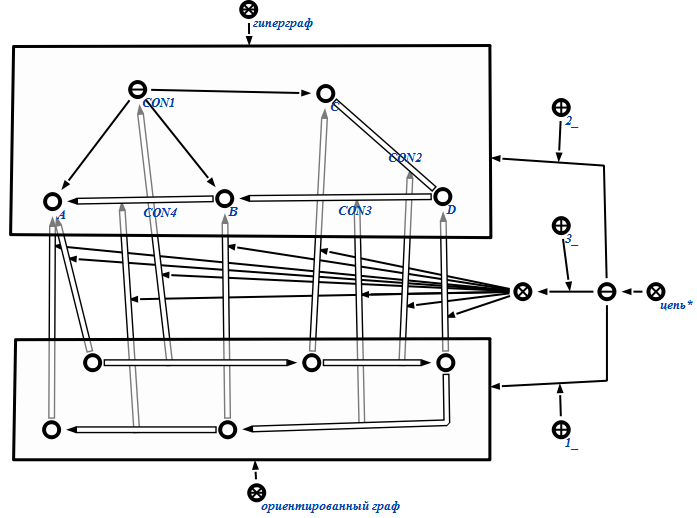
\includegraphics[scale=0.8]{2/concept/Trail}
    \label{fig:Concept_Trail}
  \end{figure}

\newpage
 
\item Простая цепь, путь (относительное понятие, бинарное
  ориентированное отношение) – это цепь, в которой все вершины
  различны. В примере ниже показан путь \idtf{A}, \idtf{CON1},
  \idtf{C}, \idtf{CON2}, \idtf{D}, \idtf{CON3}, \idtf{B} в гиперграфе.

  \begin{figure}[h!]
    \centering
    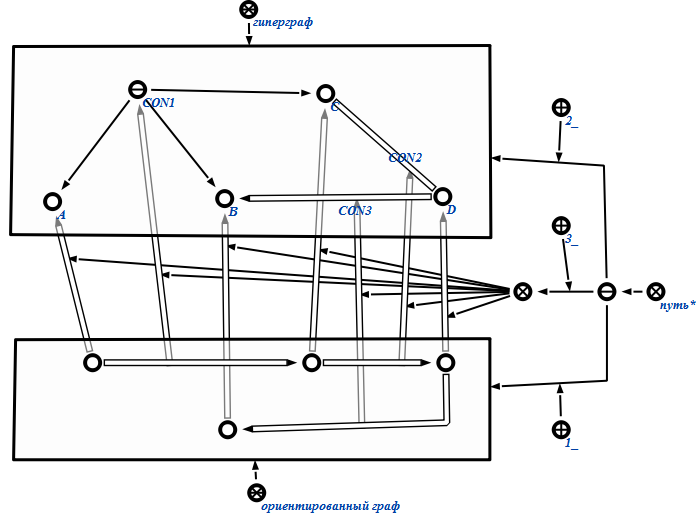
\includegraphics[scale=0.8]{2/concept/Path}
    \label{fig:Concept_Path}
  \end{figure}

\end{itemize}

\newpage

\subsection{Тестовые примеры}
\label{sec:Onto_ex_tests}

Во всех тестах графы будет приведены в сокращенной форме со скрытыми
ролями элементов графа.

\newcounter{ontotests}

\newenvironment{test}
{
  \addtocounter{ontotests}{1}

  \newpage
  \subsubsection{Тест \arabic{ontotests}}
}
{
}

\newcommand{\testnum}{\arabic{ontotests}}

\newcommand{\testin}[2][1.0]
{
  \begin{figure}[h!]
    \centering
    \includegraphics[scale=#1]{2/test/#2_In}
    \label{fig:Test#2_In}
  \end{figure}
}

\newcommand{\testout}[2][1.0]
{
  \begin{figure}[h!]
    \centering
    \includegraphics[scale=#1]{2/test/#2_Out}
    \label{fig:Test#2_Out}
  \end{figure}
}

\begin{test}
  \textbf{Вход:} Необходимо найти минимальный путь между вершинами $A$
  и $C$.

  \testin\testnum

  \textbf{Выход:} Будет найден единственный минимальный путь $A$,
  $E1$, $B$, $E2$, $C$:

  \testout\testnum
\end{test}

\begin{test}
  \textbf{Вход:} Необходимо найти минимальный путь между вершинами $A$
  и $F$.

  \testin[0.8]\testnum

  \textbf{Выход:} Будет найден один из двух минимальный путь $A$,
  $E2$, $B$, $E3$, $D$, $E5$, $F$:

  \testout[0.8]\testnum
\end{test}

\begin{test}
  \textbf{Вход:} Необходимо найти минимальный путь между вершинами $A$
  и $K$.

  \testin\testnum

  \textbf{Выход:} Минимального пути между вершинами $A$ и $K$ не
  существует. Программа должна вернуть ошибку вызывающему контексту.
\end{test}

\begin{test}
  \textbf{Вход:} Необходимо найти минимальный путь между вершинами
  $V5$ и $V11$.

  \testin[0.8]\testnum

  \textbf{Выход:} Будет найден один из двух минимальный путь $V5$,
  $E8$, $V7$, $E9$, $V6$, $E11$, $V9$, $E15$, $V11$:

  \testout[0.8]\testnum
\end{test}

\begin{test}
  \textbf{Вход:} Необходимо найти минимальный путь между вершинами
  $V1$ и $V9$.

  \testin[0.8]\testnum

  \textbf{Выход:} Минимального пути между вершинами $V1$ и $V9$ не
  существует. Программа должна вернуть ошибку вызывающему контексту.
\end{test}

%%% Local Variables: 
%%% mode: latex
%%% TeX-master: "main"
%%% End: 

\chapter{Демонстрация работы программы решения теоретико-графовой
  задачи в семантической памяти}

\section{Задание}

На этом этапе выполнения расчетной работы вам необходимо будет
продемонстрировать пошаговое выполнение алгоритма в sc-памяти. Сам
алгоритм и структуры данных для него вы уже исследовали на предыдущих
этапах расчетной работы, а сейчас надо будет продемонстрировать
графодинамику выполнения алгоритма. Это значит, что вся информация,
необходимая для работы вашего алгоритма, должна храниться в sc-памяти
и там же и обрабатываться. В качестве примера <<неудобства>>, которое
вам может принести такое требование, я могу привести невозможность
использования привычной матрицы смежности/инцидентности.  Поэтому для
прохождения этого этапа вам придется взглянуть на алгоритм, решающий
выбранную задачу, под другим углом.

\section{Волновой алгоритм поиска одного из минимальных путей в
  неориентированном графе}

\subsection{Описание алгоритма}
\label{sec:-Algo_desc}

Алгоритм поиска одного из минимальных путей в неориентированном графе
является волновым и основан на понятии волны. В рамках этого алгоритма
волной называется множество вершин, каждая из которых является в
обрабатываемом графе смежной хотя бы одной вершине из предыдущей
волны. Волна, для которой нет предыдущей волны, называется начальной и
состоит из вершины, от которой начинается поиск минимального
пути. Волна, включающая конечную вершину пути, называется
конечной. Таким образом, наш алгоритм можно задать следующим перечнем
шагов:

\begin{enumerate}
\item Добавить все вершины графа, кроме начальной вершины пути, во
  множество непроверенных вершин.
\item Создать новую волну и добавить в нее начальную вершину пути.
\item Начальная волна – это новая волна. Новой волной будем называть
  последнюю созданную волну.
\item Сформировать следующую волну для новой волны. В нее попадет та
  вершина, которая является смежной вершине из новой волны и
  присутствует во множестве непроверенных вершин. Если вершина попала
  в формируемую волну, то ее надо исключить из множества непроверенных
  вершин. Созданную волну установить как следующую для новой волны, и
  после этого созданную волну считать новой волной.
\item Если новая волна пуста, то между вершинами не существует
  пути. Завершить алгоритм.
\item Если в текущей волне есть конечная вершина, то перейти к пункту
  7, иначе к пункту 4.
\item Сформировать один из минимальных путей, проходя в обратном
  порядке по списку волн. Завершить алгоритм.
\end{enumerate}

\subsection{Пример выполнения алгоритма в sc-памяти}

\subsubsection{Соглашения по демонстрации}

Перед демонстрацией выполнения алгоритма в sc-памяти нам необходимо
установить некоторые соглашения по формирование SCg-рисунков.

При записи графов я буду использовать сокращенную форму - атрибуты для
вершин и связок не приводятся, однако вы должны помнить, что
сокращенная форма используется только для наглядности.

В качестве программных переменных, которые используются в ходе работы
алгоритма, я буду использовать sc-переменные. Для указания значения
sc-переменной используется отношение \rel{значение}.  На рисунке 3.1
задано значение для sc-переменной \vidtf{beg\_vertex}.

\begin{figure}[h!]
  \centering
  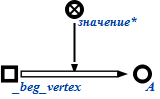
\includegraphics{images/3/Value_sc_var}
  \caption{Пример указания значения sc-переменной \vidtf{beg\_vertex}}
  \label{fig:Value_sc_var}
\end{figure}

Однако я буду сокращать способ, показанный на
рис.~\ref{fig:Value_sc_var}, опуская знак отношения
\rel{значение}. Таким образом, будет использована форма, показанная на
рис.~\ref{fig:Short_value_sc_var}. Имейте в виду, что полученная
sc-конструкция не является корректной в семантическом смысле, но в
данном разделе использование именно такой формы позволит сделать
рисунки более понятными.

\begin{figure}[h!]
  \centering
  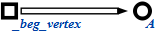
\includegraphics{images/3/Short_value_sc_var}
  \caption{Пример сокращенного указания значения sc-переменной
    \vidtf{beg\_vertex}}
  \label{fig:Short_value_sc_var}
\end{figure}

Последнее, о чем мы договоримся, будет использование цветов с целью
явного выделения изменений, произошедших с sc-конструкцией. Для этого
я буду использовать следующий перечень цветов:

\begin{itemize}
\item \textcolor{magenta}{фиолетовым} цветом будут выделяться sc-переменные, значение
  которых изменилось;
\item \textcolor{green}{зеленым} цветом будут выделяться созданные sc-элементы;
\item \textcolor{blue}{синим} цветом будут выделяться измененные sc-элементы (например,
  sc-множества, в которые был включен или из которых был исключен
  элемент).
\end{itemize}

Пришло время посмотреть, как же работает наш алгоритм в sc-памяти.

\subsubsection{Демонстрация алгоритма}

Выполнение алгоритма я продемонстрирую через состояния sc-памяти на
каждом элементарном этапе решения задачи. Для всех элементарных
этапов, для которых это возможно, в конце их краткого описания в
скобках будет указан соответствующий номер шага алгоритма из раздела
\ref{sec:-Algo_desc}.

\newenvironment{algostep}[3]
{
  \newpage
  \emph{\textbf{#1}}

  \begin{figure}[h!]
    \centering
    \includegraphics[scale=#3]{images/3/#2}
    \label{fig:#2}
  \end{figure}
}


\begin{algostep}{Задание входного графа, начальной и конечной вершины
    пути для работы алгоритма}{S1_Input_graph}{0.8}
  
  Переменные изменятся следующим образом:

  \begin{itemize}
  \item \vidtf{graph} получит в качестве значения sc-узел
    неориентированного графа;
  \item \vidtf{beg\_vertex} получит в качестве
    значения вершину А, которая будет начальной для поиска минимального
    пути;
  \item \vidtf{end\_vertex} получит в качестве значение вершину $F$,
    которая будет конечной для поиска минимального пути.  Таким образом,
    из состояния sc-памяти на этом шаге вам должно быть ясно, что будет
    производиться поиск минимального пути между вершинами $A$ и $F$.
  \end{itemize}
\end{algostep}


\begin{algostep}{Создание множества непроверенных вершин (Шаг
    1)}{S2_Create_unchecked_vertexes_set}{0.8}

  Переменная \vidtf{not\_checked\_vertexes} получит в качестве значения
  множество непроверенных вершин обрабатываемого графа (в это множество
  не включена начальная вершина пути $A$).
\end{algostep}


\begin{algostep}{Создание волны, включающей начальную вершину A (Шаги
    2, 3)}{S3_Create_1st_wave}{0.8}

  На этом этапе программа создает первую волну из списка волн. Первая
  волна содержит только начальную вершину пути $A$. Переменная
  \vidtf{new\_wave} получает в качестве значения созданную волну, и в
  будущем будет всегда указывать на вновь созданную волну.

  Переменная \vidtf{waves\_list\_head} указывает на начальный элемент
  списка волн, а переменная \vidtf{waves\_list\_tail} сейчас и в
  последующих шагах – на концевой элемент списка волн.
\end{algostep}


\begin{algostep}{Создание волны, включающей вершины B и С (Шаг
    4)}{S4_Create_next_wave}{0.8}
  
  Для вершин из предыдущей волны являются смежными и входящими во
  множество проверенных вершин только вершины $B$ и $С$. Из них
  формируем новую волну. Обратите внимание на то, что эти вершины
  исключаются из множества непроверенных вершин (см. значение
  переменной \vidtf{not\_checked\_vertexes}).

  Переменная \vidtf{waves\_list\_tail} получает в качестве значения
  созданный элемент списка, а переменная \vidtf{new\_wave} – созданную
  волну.
\end{algostep}


\begin{algostep}{Создание волны, включающей вершину D (Шаг
    4)}{S5_Create_next_wave}{0.8}

  Для вершин из предыдущей волны является смежной и входящей во
  множество проверенных вершин только вершина $D$. Из нее формируем
  новую волну. Обратите внимание на то, что эта вершина исключается из
  множества непроверенных вершин (см. значение переменной
  \vidtf{not\_checked\_vertexes}).

  Переменная \vidtf{waves\_list\_tail} получает в качестве значения
  созданный элемент списка, а переменная \vidtf{new\_wave} – созданную
  волну.
\end{algostep}


\begin{algostep}{Создание волны, включающей вершину F (Шаги 4, 5,
    6)}{S6_Create_last_wave}{0.8}

  Для вершины из предыдущей волны является смежной и входящей во
  множество проверенных вершин только вершина $F$. Из нее формируем
  новую волну. Обратите внимание на то, что эта вершина исключается из
  множества непроверенных вершин (см. значение переменной
  \vidtf{not\_checked\_vertexes}).

  Переменная \vidtf{waves\_list\_tail} получает в качестве значения
  созданный элемент списка, а переменная \vidtf{new\_wave} – созданную
  волну.

  Так как эта волна содержит конечную вершину пути $F$, то на
  следующих этапах мы перейдем к генерации одного из найденных
  минимальных путей.
\end{algostep}


\begin{algostep}{Удаление множества непроверенных
    вершин}{S7_Erase_unchecked_vertexes_set}{0.8}
 
  Подчистим память, удалив множество непроверенных вершин (значение
  переменной \vidtf{not\_checked\_vertexes}), так как оно нам уже не
  надо.
\end{algostep}


\begin{algostep}{Создание связки отношения \rel{путь} (Шаг
    8)}{S8_Create_route_tuple}{0.7}
 
  Начинаем генерацию одного из найденных минимальных путей.

  Создадим связку отношения \rel{путь} и установим ее в качестве
  значения переменной \vidtf{route}. Переменная \vidtf{route\_struct}
  получит в качестве значения ориентированный граф структуры пути, а
  переменная \vidtf{route\_visit} – отношения посещения.
\end{algostep}


\begin{algostep}{Добавление в структуру пути посещения начальной и
    конечной вершины генерируемого пути (Шаг
    8)}{S9_Add_begin_and_end_vertexes_visit_to_route_tuple}{0.7}
 
  Добавим в структуру генерируемого пути посещения начальной вершины
  $A$ и конечной вершины $F$. Созданные посещения получат в качестве
  значения переменные \vidtf{beg\_vertex\_visit} и
  \vidtf{end\_vertex\_visit}.
\end{algostep}


\begin{algostep}{Установка переменных для 1-ой итерации цикла генерации
    структуры пути (Шаг 8)}{S10_Step_building_route_structure}{0.7}
  
  Структура пути строится, начиная с конечной вершины пути $F$.

  На этом этапе переменная \vidtf{curr\_vertex} получит в качестве
  значения текущую обрабатываемую вершину, переменная \vidtf{list\_it}
  – текущий обрабатываемый элемент списка волн, переменная
  \vidtf{curr\_wave} – текущую обрабатываемую волну.
\end{algostep}

 
\begin{algostep}{Создание посещения вершины на 1-ой итерации цикла
    генерации структуры пути (Шаг
    8)}{S11_Step_building_route_structure_add_visits}{0.7}
 
  Создадим посещение для одной из вершин из волны \vidtf{curr\_wave},
  которая является смежной вершине из переменной
  \vidtf{curr\_vertex}. Для связывающего их ребра тоже создадим
  посещение.
\end{algostep}  


\begin{algostep}{Переход ко 2-ой итерации цикла генерации структуры
    пути (Шаг 8)}{S12_Step_building_route_structure}{0.7}
 
  На этом этапе переменная \vidtf{curr\_vertex} получит в качестве
  значения вершину, для которой было создано посещение на предыдущей
  итерации. Переменная \vidtf{list\_it} – предшествующей элемент
  списка волн для значения переменной \vidtf{curr\_wave} на предыдущем
  этапе. Переменная \vidtf{curr\_wave} – обрабатываемую волну для
  элемента списка из установленного значения \vidtf{list\_it}.
\end{algostep}


\begin{algostep}{Создание посещения вершины на 2-ой итерации цикла
    генерации структуры пути (Шаг
    8)}{S13_Step_building_route_structure_add_visits}{0.7}

  Создадим посещение для одной из вершин из волны \vidtf{curr\_wave},
  которая является смежной вершине из переменной
  \vidtf{curr\_vertex}. На эту роль была выбрана вершина $С$. Для
  ребра, связывающего две вершины, тоже создадим посещение.
\end{algostep}


\begin{algostep}{Переход к 3-ей итерации цикла генерации структуры пути
    (Шаг 8)}{S14_Step_building_route_structure}{0.7}
 
  На этом этапе переменная \vidtf{curr\_vertex} получит в качестве
  значения вершину, для которой было создано посещение на предыдущей
  итерации. Переменная \vidtf{list\_it} – предшествующей элемент
  списка волн для значения переменной \vidtf{curr\_wave} на предыдущем
  этапе. Переменная \vidtf{curr\_wave} – обрабатываемую волну для
  элемента списка из установленного значения \vidtf{list\_it}.
\end{algostep}


\begin{algostep}{Создание посещения вершины на 3-ей итерации цикла
    генерации структуры пути (Шаг
    8)}{S15_Step_building_route_structure_add_visits}{0.7}
 
  Так как для вершины $A$ уже создано посещение, то делать это
  повторно алгоритм не будет. А вот посещение ребра между вершинами
  $A$ и $С$ необходимо создать.

  Структура пути создано, поэтому завершаем цикл и переходим к очистке
  sc-памяти от уже ненужных sc-конструкций.
\end{algostep}

\begin{algostep}{Удаление списка волн}{S16_Erase_waves_list}{0.7}
 
  Удалим список волн. Переменные \vidtf{list\_it},
  \vidtf{waves\_list\_head}, \vidtf{curr\_wave},
  \vidtf{waves\_list\_tail} окажутся без значений.
\end{algostep}


\begin{algostep}{Результат работы алгоритма}{S17_Result}{0.7}
 
  На данном этапе продемонстрирован результат работы алгоритма,
  значение переменной \vidtf{route} будет возвращено в вызывающий
  контекст.
\end{algostep}


%%% Local Variables: 
%%% mode: latex
%%% TeX-master: "main"
%%% End: 


\part{Курс ППвИС}

\chapter{Разработка программы решения теоретико-графовой задачи на
  языке программирования C++}

В следующем разделе я описываю выполнение второго этапа расчетной
работы на примере задачи поиска одного из минимальных путей в
неориентированном графе. Для понимания руководства студент должен
обладать следующими знаниями:

\begin{itemize}
\item базовыми знаниями по языку C++;
\item базовыми знаниями по работе с STL-контейнерами std::set,
  std::map, std::list, std::pair.
\end{itemize}

\section{Задание}

На этом этапе выполнения расчетной работы вам необходимо будет
разработать программу с использованием библиотеки моделирования
sc-памяти, которая бы решала вашу теоретико-графовую задачу на основе
формализации предметной области, проведенной на предыдущем этапе. Сам
алгоритм вы уже исследовали в прошлом семестре, но сейчас надо будет
не просто реализовать какой-то алгоритма, а адаптировать его к
графодинамическому способу обработки информации. Это значит, что вся
информация, необходимая для работы вашего алгоритма, должна храниться
в sc-памяти и там же и обрабатываться. В качестве примера
<<неудобства>>, которое вам может принести такое требование, я могу
привести невозможность использования привычной матрицы
смежности/инцидентности.  Поэтому для прохождения этого этапа вам
придется взглянуть на алгоритм, решающий выбранную задачу, под другим
углом.

В качестве тестов для написанной программы необходимо использовать
тестовые примеры, которые вы сделали в ходе предыдущего этапа
расчетной работы.

\section{Установка и настройка рабочей среды}

Для начала мы установим и настроим рабочую среду для программирования
с использованием программной модели sc-памяти и запустим
программу-пример, которая использует эту модель. Всё описанное в этой
главе программное обеспечение можно найти как в интернете, так и на
кафедральном сервере info. На сервере info весь материал и всё
программное обеспечение располагается по следующему пути:
\begin{verbatim}
\\Info\StudInfo\~Методическое обеспечение кафедры\~Учебные курсы\2 курс\ППвИС\@Расчётная работа
\end{verbatim}

Во-первых, нам необходимо скачать и установить программный модуль
sc-core, который представляет собой ядро для обработки
sc-текстов. Инсталлятор для этого модуля можно взять в следующих
местах:

\begin{itemize}
\item скачать из папки
  \href{http://sourceforge.net/projects/ostis/files/kpm/}{kpm}
  sc-core-0.2.5-win32.exe (работает с MS Visual Studio 9)
\item скачать по следующему пути sc-core-0.2.5.exe (работает с MS
  Visual Studio 9):
\begin{verbatim}
\\Info\StudInfo\~Методическое обеспечение кафедры\~Учебные курсы\2 курс\ППвИС\@Расчётная работа\sc-core-0.2.5.exe
\end{verbatim}
\item скачать по следующему пути sc-core-0.2.5-vc10-bin-win32.exe
  (работает с MS Visual Studio 10):
\begin{verbatim}
\\Info\StudInfo\~Методическое обеспечение кафедры\~Учебные курсы\2 курс\ППвИС\@Расчётная работа\sc-core-0.2.5-vc10-bin-win32.exe
\end{verbatim}
\end{itemize}

После того, как вы скачали инсталлятор, запустите его. Желательно
устанавливать sc-core так, чтобы полный путь к установленной папке не
содержал пробелов в именах директорий. При установке необходимо
выбрать опцию, которая добавит директорию исполняемых файлов sc-core в
переменную среды окружения \verb+PATH+ (см. рис.~\ref{fig:Add_sc_core_to_path}).

\begin{figure}[h]
  \centering
  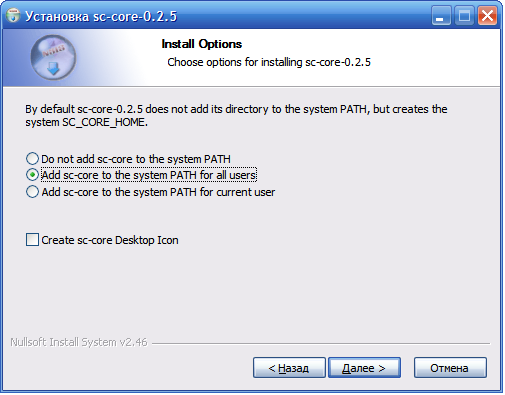
\includegraphics[scale=0.7]{images/4/setup/Add_sc_core_to_path}
  \caption{Добавление директории исполняемых файлов sc-core в
    системную переменную PATH для всех пользователей}
  \label{fig:Add_sc_core_to_path}
\end{figure}
 
Мной была выбрана установка sc-core в папку
\verb+"c:\\sc-core"+. После установки данного модуля были изменены
следующие переменные среды окружения:
\begin{itemize}
\item \verb+SC_CORE_HOME+, которая теперь имеет значение
  \verb+"c:\sc-core"+
\item \verb+PATH+, к которой была добавлена директория
  \verb+"c:\sc-core\bin"+
\end{itemize}

В дальнейшем для указания пути к директории sc-core я буду
использовать значение переменной среды окружения \verb+SC_CORE_HOME+.

Для сборки примера нам еще будет необходима программа
CMake. Необходимо скачать установочный файл для версии не ниже 2.6.2
или взять инсталлятор из папки расчетной работы на сервере info. Как и
при установке sc-core, при установке CMake необходимо выбрать опцию,
которая добавит директорию исполняемых файлов в переменную среды
окружения \verb+PATH+ (см. рис.~\ref{Add_cmake_to_path}).
 
\begin{figure}[h]
  \centering
  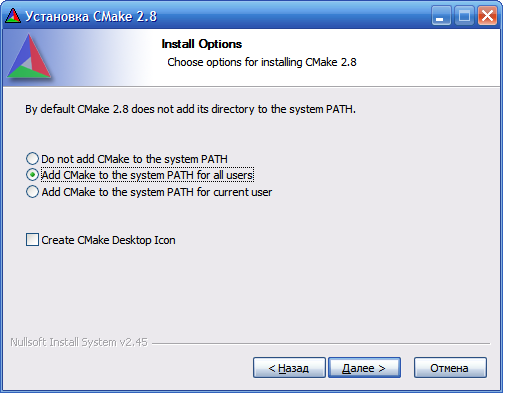
\includegraphics[scale=0.7]{images/4/setup/Add_cmake_to_path}
  \caption{Добавление CMake в системную переменную PATH для всех
    пользователей}
  \label{fig:Add_cmake_to_path}
\end{figure}

С модулем sc-core версии 0.2.5 идет старая версия примера
использования библиотеки моделирования sc-памяти, поэтому я рекомендую
вам взять из папки на сервере info файл с именем
\verb+wave_find_path.cpp+ и скопировать его в приеденную ниже папку,
заменив существующий там файл с таким именем. После этого перейдем к
генерации проекта для примера:
\begin{verbatim}
%SC_CORE_HOME%\examples\wave_find_path
\end{verbatim}

Для генерации проекта примера воспользуемся консолью. Для запуска
консоли нажимаем клавиши \verb|Win + R|, в появившемся диалоге пишем cmd и
нажимаем Enter. На экране должно появиться следующее окно, как
показано на рисунке 2.3.

\begin{figure}[h]
  \centering
  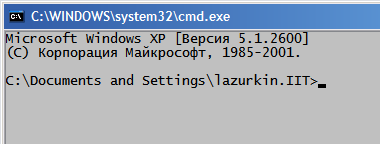
\includegraphics[scale=0.7]{images/4/setup/Run_console}
  \caption{Открытая консоль}
  \label{fig:Run_console}
\end{figure}

Переходим в директорию примера использования библиотеки моделирования
sc-памяти, используя команды:
\begin{verbatim}
c: 
cd %SC_CORE_HOME%\examples\wave_find_path
\end{verbatim}

%\begin{figure}[h]
%  \centering
%  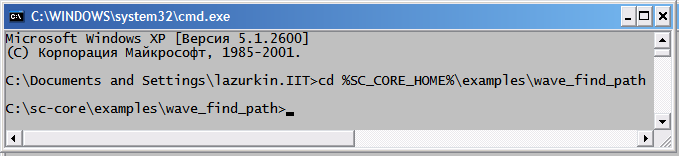
\includegraphics[scale=0.7]{images/4/setup/Cd_to_example_dir}
 % \caption{Переход в директорию примера wave\_find\_path}
  %\label{fig:Cd_to_example_dir}
%\end{figure}

% Если у вас Windows с русификацией, то могут возникнуть проблемы с запуском cmake. CMake будет сообщать о том, что он не может скопировать файлы "CMakeVSMacros1.vsmacros" и "CMakeVSMacros2.vsmacros" в "c:\Documents and Settings\lazurkin.IIT\Мои документы\Visual Studio 2008\Projects\VSMacros80\CMakeMacros" (это путь на моей файловой системе с моим именем пользователя, для вас он будет отличаться названием директории вашего пользователя). Эти файлы необходимо скопировать вручную. Для этого просто скопируйте содержимое "c:\Program Files\cmake2.8\share\cmake-2.8\Templates\" в "c:\Documents and Settings\lazurkin.IIT\Мои документы\Visual Studio 2008\Projects\VSMacros80\CMakeMacros" (этот путь для вас будет другой!!!). 

% При помощи следующей команды сгенерируем проект MS Visual Studio 9.0
% для сборки и запуска примера (в cmake есть генератор и для MS Visual
% Studio 10.0, просто введите команду cmake и на консоль будет выведен
% список всех доступных генераторов):

% cmake -G "Visual Studio 9 2008" .

 
% Рисунок 2.5 Генерация проекта для примера wave_find_path 
% Если у вас MS Visual Studio 2010, то можете попробовать команду:
% cmake .

% После корректной работы CMake в директории будет создан проект wave_find_path. Открываем его при помощи MS Visual Studio 9.0. Нажимаем правой кнопкой мыши на проекте wave_find_path в Solution Explorer и выбираем пункт меню "Set as StartUp Project". После этого название данного проекта будет выделено жирным цветом. Теперь можно запустить на исполнение пример wave_find_path (пример вывода на рисунке 2.6).
 
% Рисунок 2.6 Вывод работы программы-примера wave_find_path

\section{Назначение и структура модуля sc-core}

Модуль sc-core – это набор библиотек и программ, которые составляют
ядро обработки sc-текстов. В него входят следующие динамические
библиотеки:
\begin{itemize}
\item libsys : библиотека, обеспечивающая независимость от
  операционной системы;
\item libtgf : библиотека обработки формата TGF (Transfer Graph Format);
\item libsc : библиотека моделирования sc-памяти;
\item libpm : библиотека процессорного модуля для обработки sc-текстов
  (например, она включает scp-интерпретатор и навигационно-поисковую
  машину);
\item librgp : библиотека удаленного подключения к sc-памяти по
  протоколу RGP (Remote Graph Protocol).
\end{itemize}

Также модуль sc-core включает следующие программы:
\begin{itemize}
\item start-pm : средство запуска процессорного модуля из консоли;
\item dumptgf : утилита для просмотра TGF-файлов в человеко-читаемой
  форме;
\item scs2tgf : транслятор sc.s-текстов в формат TGF.
\end{itemize}

Как вы уже знаете, при установке инсталлятор модуля sc-core создает
переменную среды \verb+SC_CORE_HOME+, которая в качестве своего значения
будет иметь путь к корневой папке установленного модуля. Если вы
заглянете в эту папку, то сможете увидеть следующую структуру папок и
файлов (пути даются относительно значения переменной окружения
\verb+SC_CORE_HOME+):
\begin{itemize}
\item \verb|bin/| : бинарные файлы библиотек и программ. В этой директории
  динамические библиотеки для отладочной версии приложения имеют в
  конце имени букву «d» (сравните, libSCd.dll и libSC.dll);
\item \verb|doc/| : doxygen-документация на английском языке по модулю sc-core;
\item \verb|examples/| : примеры использования модуля:
  \begin{itemize}
  \item \verb|wave_find_path/| : С++-пример использования библиотеки
    sc-памяти libsc на основе алгоритма поиска одного из минимальных
    путей в неориентированном графе;
  \item \verb|fs_repo_src/| : SCP-пример на основе алгоритма поиска одного из
    минимальных путей в неориентированном графе;
  \end{itemize}
\item \verb|include/| : содержит директории с заголовочными файлами для всех библиотек
  модуля;
\item \verb|lib/| : библиотеки импорта для всех динамических библиотек модуля
  В этой директории библиотеки импорта для отладочной версии
  динамической библиотеки имеют в конце имени букву «d» (сравните,
  libSCd.lib и libSC.lib);
\item \verb|share/| : содержит дополнительные необходимые ресурсы для работы
  модуля, которые нельзя отнести ни в одну из уже описанных
  директорий.
\end{itemize}

Из всего описанного выше в контексте данного руководства нас будет
интересовать библиотека моделирования sc-памяти libsc и пример ее
использования \verb|wave_find_path|. В ходе дальнейшего разговора мы сначала
будем рассматривать основные понятия, структуру и классы библиотеки
libsc, а затем перейдем к более конкретному рассмотрению примера
использования этой библиотеки.

\section{Библиотека моделирования sc-памяти – libsc}

В данном разделе мы рассмотрим библиотеку моделирования sc-памяти в
объеме, необходимом для выполнения это этапа расчетной работы.

\subsection{Общие сведения}

Библиотека моделирования sc-памяти написана на языке C++, поэтому в
этом разделе мы будем рассматривать в основном классы для
моделирования sc-памяти и их методы, а также некоторые функции попадут
в поле нашего зрения. Однако сейчас давайте рассмотрим файлы и
директории из модуля sc-core, которые имеют отношение к библиотеке. И
так, приступим (пути даются относительно значения переменной окружения
\verb|SC_CORE_HOME|):
\begin{itemize}
\item \verb|bin/libSCd.dll| : debug-версия динамической библиотеки
  моделирования sc-памяти;
\item \verb|bin/libSC.dll| : release-версия динамической библиотеки
  моделирования sc-памяти;
\item \verb|lib/libSCd.lib| : библиотека импорта для динамической библиотеки
  libSCd.dll;
\item \verb|lib/libSC.lib| : библиотека импорта для динамической библиотеки
  libSC.dll;
\item \verb|doc/sc-core/| : общая doxygen-документация по модулю
  sc-core, в том числе и по рассматриваемой библиотеке libsc;
\item \verb|include/libSC/| : заголовочные файлы рассматриваемой
  библиотеки;
\item \verb|examples/wave_find_path| : пример использования
  рассматриваемой библиотеки.
\end{itemize}

Библиотека libsc зависит от библиотеки обработки формата TGF libtgf, к
которой относятся следующие директории и папки (пути даются
относительно значения переменной окружения \verb|SC_CORE_HOME|):

\begin{itemize}
\item \verb|bin/libTGFd.dll| : debug-версия динамической библиотеки
  libtgf (она необходима для работы с libSCd.dll);
\item \verb|bin/libTGF.dll| : release-версия динамической библиотеки
  libtgf (она необходима для работы с libSC.dll);
\item \verb|include/libTGF/| : заголовочные файлы библиотеки libtgf;
\end{itemize}

Теперь перейдем к непосредственному описанию библиотеки libsc.

\subsection{Сегментная модель sc-памяти}

Когда вы занимались формализацией на SCg по курсу МОИС, то считали,
что sc-элементы с одинаковыми идентификаторами должны
склеиться. Однако в реализации sc-памяти используется сегментная
модель и поэтому всё несколько сложнее.

В сегментной модели вся память разбивается на sc-сегменты, где каждый
sc-элемент принадлежит ровно одному сегменту. Уникальность
идентификаторов sc-элементов имеет место только в рамках
sc-сегмента. Сами sc-сегменты могут организовываться в рамках
sc-директории. Проиллюстрирую на конкретной структуре sc-памяти:

\begin{itemize}
\item /: корневая sc-директория, которая всегда существует
  
  \begin{itemize}
  \item \verb|graph_theory/|: sc-директория, которая содержит базу знаний по
    теории графов
    \begin{itemize}
    \item \verb|keynode|: sc-сегмент, который содержит ключевые
      узлы базы знаний по теории графов
      \begin{itemize}
      \item \idtf{графовая структура}
      \item \idtf{вершина\_}
      \item \idtf{связка\_}
      \item \idtf{неориентированный граф}
      \item \idtf{ребро\_} и т.д.
      \end{itemize}
    \end{itemize}

  \item \verb|tmp/|: содержит sc-сегменты для временной обработки
    sc-конструкций
    \begin{itemize}
    \item \verb|wave_find_path| : временный sc-сегмент для работы алгоритма
      поиска одного из минимальных путей в неориентированном графе
    \end{itemize}

  \item \verb|proc/|: содержит системные sc-сегменты;
    \begin{itemize}
    \item \verb|keynode|: sc-сегмент, который содержит системные ключевые
      узлы
      \begin{itemize}
      \item \idtf{1\_}
      \item \idtf{2\_} и т.д.
      \end{itemize}
    \end{itemize}
  \end{itemize}
\end{itemize}

Такая структура sc-директорий и sc-сегментов аналогична структуре
папок и файлов на файловой системе. Аналогом файла является
sc-сегмент, а аналогом содержимого файла является sc-конструкции. В
сегментной модели любой объект (sc-директория, sc-сегмент, sc-элемент)
может быть однозначно идентифицирован при помощи строки особого вида,
которая по историческим причинам называется URI (Universal Resource
Identifier). Формат URI аналогичен формату пути к папке или файлу на
файловых системах Unix-подобных операционных систем. Вот некоторые
примеры URI:

\begin{itemize}
\item \verb|/|: URI sc-директории
\item \verb|/graph_theory/keynode| : URI sc-сегмента
\item \verb|/graph_theory/keynode/вершина_| : URI sc-элемента
\end{itemize}

Адресация sc-элементов с использованием URI удобна для человека, но
неудобна для компьютера, поэтому существует понятие
sc-адреса. SC-адрес – это некоторое число, которое однозначно
идентифицирует sc-элемент в сегментной модели sc-памяти. С
использованием sc-адресов sc-элементов ведется их обработка в рамках
sc-сессии. SC-сессия - это логически единая последовательность
операций над некоторой областью sc-памяти (sc-директориями,
sc-сегментами, sc-элементами). Для того, чтобы получить доступ к
данным sc-сегмента, нужный sc-сегмент должен быть открыт в рамках
используемой sc-сессии. Существует особый вид sc-сессии, который
называется системная sc-сессия, в рамках которой все существующие
sc-сегменты всегда открыты.

Я думаю, что читатель уже получил общие сведения о том, что такое
сегментная модель, sc-директория, sc-сегмент, URI, sc-адрес,
sc-сессия, поэтому в следующем разделе я начну рассматривать
практические вопросы использования библиотеки моделирования sc-памяти.

\subsection{Начало работы с библиотекой libsc}

В прошлом разделе мы рассмотрели логическое устройство сегментной
модели sc-памяти, а теперь проведем аналогию с текущей реализацией на
языке программирования С++.

Понятию sc-сегмента в библиотеке libsc соответствует класс
\lstinline{sc_segment}, который описан в файле
\verb|sc_segment.h|. Понятию sc-адреса соответствует
\lstinline{typedef sc_addr} из заголовочного файла \verb|sc_types.h|,
а sc-сессии – класс \lstinline{sc_session} из \verb|libsc.h|. Для
представления URI и идентификаторов sc-элементов используется
\lstinline{typedef sc_string} (это просто другое имя для
\lstinline{std::string}), объявленный в \verb|sc_types.h|. Чтобы
начать работу со всеми этими типами, достаточно подключить только один
заголовочный файл, а именно \verb|libsc.h|, потому что в него включены
и \verb|sc_segment.h|, и \verb|sc_types.h|.

Работа с объектами классов \lstinline{sc_session} и
\lstinline{sc_segment} всегда ведется через указатель на объект,
поэтому методы и функции, которые возвращают указатель на объекты этих
классов, могут возвращать \lstinline{0} или \lstinline{NULL}, чтобы
показать наличие ошибки в процессе выполнения. Если в тексте ниже я
буду писать о работе с объектами классов \lstinline{sc_session} и
\lstinline{sc_segment}, то это почти всегда надо понимать, как работу
с такими объектами через указатель.

Рассмотрим, как обстоят дела в этом плане с типом
\lstinline{sc_addr}. В \verb|sc_types.h| он объявлен следующим образом:
\begin{lstlisting}
  typedef sc_global_addr *sc_addr;
\end{lstlisting}

Как видно из приведенного выше объявления, \lstinline{sc_addr} – это
указатель на класс \lstinline{sc_global_addr}. Поэтому методы и
функции, которые возвращают \lstinline{sc_addr}, могут возвращать
\lstinline{0}, \lstinline{NULL} или \lstinline{SCADDR_NIL} (это
\lstinline{define} для \lstinline{0}), чтобы показать наличие ошибки в
процессе выполнения. В отличие от \lstinline{sc_session} и
\lstinline{sc_segment}, с типом \lstinline{sc_addr} мы работаем без
указателя, потому что \lstinline{sc_addr} – это и так указатель
(просто другое имя для указателя на
\lstinline{sc_global_addr}). Напоследок об \lstinline{sc_addr} стоит
сказать следующее:
\begin{itemize}
\item для переменных этого типа можно использовать операторы
  \lstinline{==} и \lstinline{!=}, чтобы проверить идет работа с одним
  и тем же sc-элементом или с разными;
\item у \lstinline{sc_global_addr} есть открытое поле
  \lstinline{sc_global_addr::seg}, которое позволяет получить
  sc-cегмент, в котором находится адресуемый sc-элемент;
\item если в дальнейшем будет идти речь о работе с sc-элементами, то
  это значит, что речь идет о работе с соответствующими им
  sc-адресами.
\end{itemize}

Предыдущий текст должен был вас уже утомить, поэтому разбавим этот
раздел примерами кода. Для начала работы с моделью sc-памяти ее надо
инициализировать, это можно сделать вот так:

\begin{lstlisting}[texcl]
  #include <libsc.h>

  // $\dots$
  // Инициализируем sc-память при помощи функции \verb|libsc_init|.
  // Она вернет системную sc-сессию.
  // 
  sc_session *system = libsc_init();
\end{lstlisting}

Теперь необходимо инициализировать системные ключевые узлы (например,
\idtf{1\_}, \idtf{2\_} и др.). Все системные ключевые узлы объявлены в
заголовочном файле \verb|pm_keynodes.h| и инициализируются функцией
\lstinline{pm_keynodes_init}:

\begin{lstlisting}[texcl]
  #include <pm_keynodes.h>

  // $\dots$
  // Ключевые узлы будут созданы в sc-сегменте "/proc/keynode".
  // Например:
  //  - для работы с ключевым узлом \idtf{1\_} можно использовать имя \verb|N1_|
  //  - для работы с ключевым узлом \idtf{2\_} можно использовать имя \verb|N2_|
  //  - закономерность очевидна $\dots$
  //
  pm_keynodes_init(system);
\end{lstlisting}

В принципе уже можно работать с sc-памятью через системную sc-сессию
\lstinline{system}, но в идеале лучше работать через пользовательскую
sc-сессию:

\begin{lstlisting}[texcl]
  // Получим пользовательскую sc-сессию при помощи функции \verb|libsc_login|.
  //
  sc_session *session = libsc_login();

  // При помощи метода \verb|sc_session::open_segment| по URI "/proc/keynode"
  // откроем в нашей пользовательской sc-сессии sc-сегмент системных 
  // ключевых узлов.
  //
  session->open_segment(“/proc/keynode”);
\end{lstlisting}

Теперь создадим уникальный sc-сегмент для исследования работы
sc-памяти:

\begin{lstlisting}[texcl]
  // Этот заголовочный файл содержит функции, которые облегчают работу с 
  // sc-сегментами.
  #include <segment_utils.h>
  
  // $\dots$
  // Создадим уникальный sc-сегмент с использованием \verb|create_unique_segment|
  // и URI этого sc-сегмента будет начинатся с "/tmp/test".
  // 
  sc_segment *segment = create_unique_segment(session, “/tmp/test”);

  // Созданный при помощи sc-сессии session sc-сегмент будет автоматический
  // открыт в ней.
  //
\end{lstlisting}

Пользовательская sc-сессия \lstinline{session} и созданный sc-сегмент
\lstinline{segment} будут использоваться во всех дальнейших примерах
без какого-то явного объявления.

После окончания необходимой работы sc-память нужно почистить:
\begin{lstlisting}[texcl]
  // Удалим созданный sc-сегмент seg при помощи метода \verb|sc_session::unlink|
  // Метод \verb|sc_segment::get_full_uri| возвращает URI sc-сегмента.
  //
  session->unlink(segment->get_full_uri());

  // Закроем пользовательскую sc-сессию.
  //
  session->close();

  // Деинициализируем sc-память.
  //
  libsc_deinit();

  // Обратите внимани на то, что явно при помощи оператора \verb|delete| никакая 
  // память не освобождается. При работе с типами \verb|sc_session|, \verb|sc_segment|,
  // \verb|sc_addr| память явно освобождать не надо.
  //
\end{lstlisting}

Перед тем, как мы будем рассматривать операции генерации и поиска в
sc-памяти, вам еще нужно познакомиться со способом задания типа
sc-элементов, поэтому переходим к следующему разделу.

\subsection{Тип sc-элемента}

Для задания типа sc-элемента в библиотеке libsc используется С++-тип
\lstinline{sc_type}, который объявлен в файле
\verb|sc_types.h|. Значение типа \lstinline{sc_type} – это просто
число, которое является результатом операции побитового ИЛИ некоторых
числовых констант. Каждая из числовых констант задает значение
свойства из заранее определенного диапазона. Для выполнения расчетной
работы вам достаточно знать о следующих свойствах:

\begin{itemize}
\item Структурный тип sc-элемента. Используемые числовые константы
  С++:
  \begin{itemize}
  \item \lstinline{SC_UNDF}: sc-элемент неопределенного типа;
  \item \lstinline{SC_ARC}: sc-дуга;
  \item \lstinline{SC_NODE}: sc-узел.
  \end{itemize}

\item Константность sc-элемента. Используемые числовые константы С++:
  \begin{itemize}
  \item \lstinline{SC_CONST}: константность;
  \item \lstinline{SC_VAR}: переменность;
  \item \lstinline{SC_METAVAR}: метапеременность.
  \end{itemize}

\item Нечеткость sc-дуги. Используемые числовые константы С++:
  \begin{itemize}
  \item \lstinline{SC_POS}: позитивность;
  \item \lstinline{SC_NEG}: негативность;
  \item \lstinline{SC_FUZ}: нечеткость.
  \end{itemize}
\end{itemize}

С использованием описанных выше числовых констант, например,
константный sc-узел можно задать как \lstinline{SC_NODE|SC_CONST}, а
позитивную константную sc-дугу как
\lstinline{SC_ARC|SC_CONST|SC_POS}. В таблице~\ref{tab:SCgType2SCType}
приведены соответствующие значения типа \lstinline{sc_type} для всех
необходимых SCg-элементов. Обратите внимание, что на уровне библиотеки
libsc нет разницы в кодировании структурных типов SCg-элементов
(например, константный sc-атрибут и константное sc-отношение
кодируются как константный sc-узел).

\begin{table}[ht]
  \caption{Соответствие SCg-элемента значению типа sc\_type из libsc}
  \centering
  \begin{tabular}{|c|c|}
    \hline
	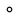
\includegraphics{images/4/scg2sc/undf_const} & \verb+SC_UNDF|SC_CONST+
    , \verb+SC_U_CONST+ \\
    
    \hline
    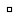
\includegraphics{images/4/scg2sc/undf_var} & \verb+SC_UNDF|SC_VAR+, \verb+SC_U_VAR+ \\
    
    \hline
    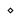
\includegraphics{images/4/scg2sc/undf_metavar} & \verb+SC_UNDF|SC_METAVAR+
    , \verb+SC_U_METAVAR+ \\
    
    \hline
    
\includegraphics{images/4/scg2sc/node_general_const}
    
\includegraphics{images/4/scg2sc/node_role_const}
    \includegraphics{images/4/scg2sc/node_struct_const}
    \includegraphics{images/4/scg2sc/node_concept_const}
    \includegraphics{images/4/scg2sc/node_binary_const}
    & \verb+SC_NODE|SC_CONST+, \verb+SC_N_CONST+ \\
    
    \hline
    \includegraphics{images/4/scg2sc/node_general_var}
    \includegraphics{images/4/scg2sc/node_role_var}
    \includegraphics{images/4/scg2sc/node_struct_var}
    \includegraphics{images/4/scg2sc/node_concept_var}
    \includegraphics{images/4/scg2sc/node_binary_var}
    & \verb+SC_NODE|SC_VAR+, \verb+SC_N_VAR+ \\
    
    \hline
    \includegraphics{images/4/scg2sc/node_general_meta}
    \includegraphics{images/4/scg2sc/node_role_meta}
    \includegraphics{images/4/scg2sc/node_struct_meta}
    \includegraphics{images/4/scg2sc/node_concept_meta}
    \includegraphics{images/4/scg2sc/node_binary_meta}
    & \verb+SC_NODE|SC_METAVAR+, \verb+SC_N_METAVAR+ \\
    
    \hline
	\includegraphics{images/4/scg2sc/arc_main} & \verb+SC_ARC|SC_CONST|SC_POS+
    , \verb+SC_A_CONST|SC_POS+ \\
    
    \hline
	\includegraphics{images/4/scg2sc/pair_const_perm_fuz} & \verb+SC_ARC|SC_CONST|SC_FUZ+
    , \verb+SC_A_CONST|SC_FUZ+ \\
    
    \hline
	\includegraphics{images/4/scg2sc/pair_const_perm_neg} & \verb+SC_ARC|SC_CONST|SC_NEG+
    , \verb+SC_A_CONST|SC_NEG+ \\
    
    \hline
	\includegraphics{images/4/scg2sc/pair_var_perm_pos} & \verb+SC_ARC|SC_VAR|SC_POS+
    , \verb+SC_A_VAR|SC_POS+ \\
    
    \hline
	\includegraphics{images/4/scg2sc/pair_var_perm_fuz} & \verb+SC_ARC|SC_VAR|SC_FUZ+
    , \verb+SC_A_VAR|SC_FUZ+ \\
    
    \hline
	\includegraphics{images/4/scg2sc/pair_var_perm_neg} & \verb+SC_ARC|SC_VAR|SC_NEG+
    , \verb+SC_A_VAR|SC_NEG+ \\
    
    \hline
	\includegraphics{images/4/scg2sc/pair_meta_perm_pos} & \verb+SC_ARC|SC_METAVAR|SC_POS+
    , \verb+SC_A_METAVAR|SC_POS+ \\
    
    \hline
	\includegraphics{images/4/scg2sc/pair_meta_perm_fuz} & \verb+SC_ARC|SC_METAVAR|SC_FUZ+
    , \verb+SC_A_METAVAR|SC_FUZ+ \\
    
    \hline
	\includegraphics{images/4/scg2sc/pair_meta_perm_neg} & \verb+SC_ARC|SC_METAVAR|SC_NEG+
    , \verb+SC_A_METAVAR|SC_NEG+ \\
    
    \hline
  \end{tabular}
  \label{tab:SCgType2SCType}
\end{table}

Для получения и установки типа sc-элемента используются методы
\lstinline{sc_session::get_type} и
\lstinline{sc_session::change_type}. Более подробную информацию о них
можно найти в doxygen-документации.

Бинарные неориентированные (рис.~\ref{fig:Binary_unorient_pair}) и
ориентированные пары (рис.~\ref{fig:Binary_orient_pair}) в текущей
версии библиотеки libsc нельзя представить в виде атомарных элементов,
а представляются они так, как показано на
рисунках~\ref{fig:Unpack_binary_unorient_pair}~и~\ref{fig:Unpack_binary_orient_pair}
соответственно.

\begin{figure}[h!]
  \centering
  \includegraphics{images/4/scg2sc/Binary_unorient_pair}
  \caption{Бинарная неориентированная пара}
  \label{fig:Binary_unorient_pair}
\end{figure}

\begin{figure}[h!]
  \centering
  \includegraphics{images/4/scg2sc/Binary_orient_pair}
  \caption{Бинарная ориентированная пара}
  \label{fig:Binary_orient_pair}
\end{figure}

\begin{figure}[h!]
  \centering
  \includegraphics{images/4/scg2sc/Unpack_binary_unorient_pair}
  \caption{Кодирование бинарной неориентированной пары}
  \label{fig:Unpack_binary_unorient_pair}
\end{figure}

\begin{figure}[h!]
  \centering
  \includegraphics{images/4/scg2sc/Unpack_binary_orient_pair}
  \caption{Кодирование бинарной ориентированной пары}
  \label{fig:Unpack_binary_orient_pair}
\end{figure}

Как видно из приеденных рисунков бинарная неориентированная пара
представляется при помощи трех, а не одного sc-элемента. Бинарная
ориентированная пара представляется при помощи пяти sc-элементов, два
из которых (sc-узлы \idtf{1\_} и \idtf{2\_}) находятся в sc-сегменте
\verb|/proc/keynode| и являются ключевыми узлами.

В следующем разделе мы рассмотрим виды основных обрабатываемых
sc-конструкций.

\subsection{Основные обрабатываемые sc-конструкции}

В sc-памяти sc-элементы могут обрабатываться как поэлементно, так и
целыми группами. Можно выделить два вида таких групп sc-элементов.

Самой распространенной является трехэлементная sc-конструкция. Она
состоит из sc-узла и sc-элемента произвольного типа, которые связаны
sc-дугой. Пример частного случая трехэлементной sc-конструкции
приведен на рис.~\ref{fig:3_sc_constr} (обратите внимание на нумерацию
элементов). Этот частный случай трехэлементной sc-конструкции включает
в качестве первого элемента - константный sc-узел, второго элемента –
константную позитивную sc-дугу, в качестве третьего элемента -
константный sc-узел.

\begin{figure}[h!]
  \centering
  \includegraphics{images/4/3_sc_constr}
  \caption{Трехэлементная sc-конструкция}
  \label{fig:3_sc_constr}
\end{figure}

Не менее распространённой является пятиэлементная sc-конструкция,
частный случай которой приведен на рис.~\ref{fig:5_sc_constr}. Этот
частный случай пятиэлементной sc-конструкции включает в качестве 1-го
элемента – константный sc-узел, 2-го элемента – константную позитивную
sc-дугу, 3-го элемента – константный sc-узел, 4-го элемента -
константную позитивную sc-дугу, 5-го элемент – константный sc-узел.

\begin{figure}[h!]
  \centering
  \includegraphics{images/4/5_sc_constr}
  \caption{Пятиэлементная sc-конструкция}
  \label{fig:5_sc_constr}
\end{figure}

Чаще всего пятиэлементная sc-конструкция используется, когда второй
элемент (sc-дуга) уточняется атрибутом, который является пятым
элементом пятиэлементной sc-конструкции.

\subsection{Генерация и удаление sc-конструкций в sc-памяти}

Для генерации одноэлементной sc-конструкции предназначен метод
\lstinline{sc_session::create_el}. Пример генерации константного
sc-узла (если sc-узел будет сгенерирован, то переменная получит в
качестве значения sc-адрес этого узла, иначе она получит в качестве
значения нулевой указатель):

\begin{lstlisting}[texcl]
sc_addr node = session->create_el(
    segment,      // sc-сегмент, в котором будет сгенерирован sc-элемент
    SC_N_CONST // тип sc-элемента
);
\end{lstlisting}

Давайте сгенерируем два константных sc-узла и присвоим им
идентификаторы при помощи метода \lstinline{sc_session::set_idtf} (для
получения идентификатора служит метод
\lstinline{sc_session::get_idtf}):

\begin{lstlisting}[texcl]
sc_addr e1 = session->create_el(segment, SC_N_CONST);
sc_addr e3 = session->create_el(segment, SC_N_CONST);

session->set_idtf(e1, "First");
session->set_idtf(e3, "Third");
\end{lstlisting}

В данной версии модели sc-памяти все sc-элементы всегда имеют
уникальный идентификатор, поэтому не удивляйтесь, если sc-элементы,
для которых вы не устанавливали идентификатор, будут иметь в качестве
него строки странного содержания. Это нормально. Вернемся к нашему
примеру.  Содержимое sc-сегмента segment после выполнение предыдущего
кода показано на рис.~\ref{fig:gen3_f_a_f_before}.

\begin{figure}
  \centering
  \includegraphics{images/4/gen/gen3_f_a_f_before}
  \caption{Содержимое sc-сегмент segment после генерации двух sc-узлов}
  \label{fig:gen3_f_a_f_before}
\end{figure}

В классе \lstinline{sc_session} есть специальный метод
\lstinline{gen3_f_a_f}, который генерирует второй элемент
трехэлементной sc-конструкции, если известны ее первый и третий
элементы. Его сигнатура выглядит следующим образом:
\begin{lstlisting}[texcl]
class sc_session
{
public:
    // $\dots$
    virtual sc_retval gen3_f_a_f(
        // sc-адрес 1-го элемент
        sc_addr e1,

        // по этому адресу поместить sc-адрес 2-го элемент
        sc_addr *e2,

        // sc-сегмент, в котором будет сгенерирован 2-ой элемент
        sc_segment *seg2,

        // тип 2-го элемента
        sc_type t2,

        // sc-адрес 3-го элемент
        sc_addr e3
    ) = 0;
    // $\dots$
};
\end{lstlisting}

Генерацию трехэлементной sc-конструкции с sc-узлами First и Third
можно провести следующим образом:
\begin{lstlisting}[texcl]
// переменная для sc-адреса 2-го элемента трехэлементной sc-конструкции.
sc_addr e2 = 0;

// Генерация sc-дуги между 1-ым и 3-им элементами.
session->gen3_f_a_f(
    // 1-ый элемент
    e1,

    // в e2 будет помещен sc-адрес 2-го элемента
    &e2,

    // sc-сегмент, в котором будет сгенерирован 2-ой элемент
    segment,

    // тип 2-ого элемента - константная позитивная sc-дуга
    SC_A_CONST|SC_POS,

    // 3-ий элемент
    e3
);
\end{lstlisting}

После выполнения приведенного выше кода содержимое sc-сегмента
\lstinline|segment| изменится так, как показано на
рис.~\ref{fig:gen3_f_a_f_after}.

\begin{figure}[h!]
  \centering
  \includegraphics{images/4/gen/gen3_f_a_f_after}
  \caption{Пример генерации трехэлементной sc-конструкции}
  \label{fig:gen3_f_a_f_after}
\end{figure}

Но в некоторых случаях нам не надо получать sc-адрес второго элемента
при использовании метода \lstinline|sc_session::gen3_f_a_f|. В этом
случае можно в качестве второго аргумента этого метода передавать
нулевой указатель:

\begin{lstlisting}[texcl]
// Генерация sc-дуги между 1-ым и 3-им элементами.
session->gen3_f_a_f(
    // 1-ый элемент
    e1,

    // использован нулевой указатель,
    // а это значит что метод не будет возвращать sc-адрес
    // 2-го элемента трехэлементной sc-конструкции
    0,

    // sc-сегмент, в котором будет сгенерирован 2-ой элемент
    segment,

    // тип 2-ого элемента - константная позитивная sc-дуга
    SC_A_CONST|SC_POS,

    // 3-ий элемент
    e3
);
\end{lstlisting}

Запомните этот прием передачи нулевого указателя, потому что он
используется во многих методах и функциях libsc, которые должны
возвращать более одного аргумента.

Теперь обратим внимание на возвращаемое значение метода
\lstinline|sc_session::gen3_f_a_f|. Оно имеет тип
\lstinline|sc_retval| (sc-код возврата) и является просто числом, по
которому можно определить код произошедшей ошибки. Тип
\lstinline|sc_retval| используется во многих методах и функция
библиотеки, и вам необходимо знать о следующих значения этого типа:


\begin{itemize}
\item Константа \lstinline|RV_OK| : функция или метод отработал
  успешно;
\item Константа \lstinline|RV_ERR_GEN| : в процессе работы функции или метода
  произошла ошибка;
\item Константа \lstinline|RV_THEN| : функция или метод сообщает о
  том, что необходим переход по then-ветке условного оператора;
\item Константа \lstinline|RV_ELSE_GEN| : функция или метод сообщает о
  том, что необходим переход по else-ветке условного оператора.
\end{itemize}

В случае успешного выполнения метод \lstinline|sc_session::gen3_f_a_f|
возвратит \lstinline|RV_OK|, а в случае неуспешного –
\lstinline|RV_ERR_GEN|. Проверки можно организовать следующим образом:
\begin{lstlisting}[texcl]
if (session->gen3_f_a_f(...) == RV_OK) {
    // Генерация прошла успешно
} else {
    // Возникла ошибка в процессе генерации
}

// Зная о том, что константа RV\_OK равна 0 можно
// организовать проверку следующим образом.
if (!session->gen3_f_a_f(...)) {
    // Генерация прошла успешно
} else {
    // Возникла ошибка в процессе генерации
}

// Зная о том, что код ошибки неравен 0 можно
// организовать проверку ошибочной ситуации следующим образом.
if (session->gen3_f_a_f(...)) {
    // Возникла ошибка в процессе генерации
}
\end{lstlisting}

Если вы не пишете какой-то специальный устойчивый код, то такие
проверки в алгоритме генерации делать нет необходимости, потому что
ошибочный код возврата метод \lstinline|sc_session::gen3_f_a_f|
возвращает в следующих случаях:
\begin{itemize}
\item не удалось выделить память под генерируемые элементы;
\item sc-сегмент, в котором происходит генерация 2-го элемент
  трехэлементной sc-конструкции закрыт в рамках данной sc-сессии или
  не существует;
\item указан неверный тип 2-го элемента трехэлементной sc-конструкции
  (2-ой элемент должен быть всегда sc-дугой);
\item sc-адреса первого и третьего sc-элементов недействительны в
  рамках данной sc-сессии (эти sc-элементы могут быть уже удалены или
  их sc-сегменты закрыты в рамках данной sc-сессии).
\end{itemize}

Напоследок давайте попробуем написать функцию
\lstinline|my_gen3_f_a_f|, которая делает то же самое, что и метод
\lstinline|sc_session::gen3_f_a_f|. Код этой функции выглядит
следующим образом:
\begin{lstlisting}[texcl]
sc_retval my_gen3_f_a_f(
    sc_session *s, // sc-сессия, через которую будет идти работа
    sc_addr e1,
    sc_addr *e2,
    sc_segment *s2,
    sc_type t2,
    sc_addr e3)
{
    // Генерация 2-го элемента
    sc_addr ce2 = s->create_el(s2, t2);
    if (!ce2)
        return RV_ERR_GEN;

    // Установка начала и конца для sc-дуги ce2
    // (2-го элемента трехэлементной sc-конструкции)
    if (s->set_beg(ce2, e1) || s->set_end(ce2, e3)) {
        // Произошла ошибка и необходимо удалить ce2
        s->erase_el(ce2);
        return RV_ERR_GEN;
    }

    if (e2)
        *e2 = ce2;

    return RV_OK;
}
\end{lstlisting}

В приведенном выше коде для вас должны быть незнакомы только методы
\lstinline|sc_session::set_beg| и \lstinline|sc_session::set_end|. Они
используются для установки начала и конца sc-дуги (для получения
начала и конца используются методы \lstinline|sc_session::get_beg| и
\lstinline|sc_session::get_end| соответственно) и объявлены следующим
образом:
\begin{lstlisting}[texcl]
class sc_session
{
public:
     // $\dots$
     virtual sc_retval set_beg(sc_addr arc, sc_addr beg) = 0;
     virtual sc_retval set_end(sc_addr arc, sc_addr end) = 0;
     // $\dots$
};
\end{lstlisting}

А теперь давайте вернем sc-сегмент \lstinline|segment| из теперешнего
состояния (рис.~\ref{fig:gen3_f_a_f_after}) в состояние, которое
показано на рис.~\ref{fig:gen3_f_a_f_before}. Для этого нам надо
удалить недавно сгенерированную константную позитивную
sc-дугу. Удаление sc-элементов обеспечивается при помощи метода
\lstinline|sc_session::erase_el|:

\begin{lstlisting}[texcl]
class sc_session
{
public:
    // $\dots$
    virtual sc_retval erase_el(sc_addr el) = 0;
    // $\dots$
};
\end{lstlisting}

Следующий код осуществит удаление sc-дуги:

\begin{lstlisting}[texcl]
session->erase_el(e2);
\end{lstlisting}

Теперь добавим еще один константный sc-узел к уже существующим двум:

\begin{lstlisting}[texcl]
sc_addr e5 = session->create_el(segment, SC_N_CONST);
session->set_idtf(e5, "Fifth");
\end{lstlisting}

После выполнения приведенного выше куска кода состояние sc-сегмента
будет таким, как показано на рис.~\ref{fig:gen5_f_a_f_a_f_before}.

\begin{figure}[h!]
  \centering
  \includegraphics{images/4/gen/gen5_f_a_f_a_f_before}
  \caption{Содержимое sc-сегмента segment после генерации третьего sc-узла ла}
  \label{fig:gen5_f_a_f_a_f_before}
\end{figure}

В классе \lstinline|sc_session| есть специальный метод
\lstinline|gen5_f_a_f_a_f|, который генерирует второй и четвертый
элементы пятиэлементной sc-конструкции, если известны ее первый,
третий и пятый элементы. Его сигнатура выглядит следующим образом:

\begin{lstlisting}[texcl]
class sc_session
{
public:
    // $\dots$
    virtual sc_retval gen5_f_a_f_a_f(
        // sc-адрес 1-го элемент
        sc_addr e1,

        // по этому адресу поместить sc-адрес 2-го элемент
        sc_addr *e2,

        // sc-сегмент, в котором будет сгенерирован 2-ой элемент
        sc_segment *seg2, 

        // тип 2-го элемента
        sc_type t2,

        // sc-адрес 3-го элемент
        sc_addr e3,

        // по этому адресу поместить sc-адрес 4-го элемент
        sc_addr *e2,

        // sc-сегмент, в котором будет сгенерирован 4-ой элемент
        sc_segment *seg4,

        // тип 4-го элемента
        sc_type t4,

        // sc-адрес 5-го элемент
        sc_addr e5
    ) = 0;
    // $\dots$
};
\end{lstlisting}

Генерацию пятиэлементной sc-конструкции с sc-узлами \vidtf{First},
\vidtf{Third}, \vidtf{Fifth} можно провести следующим образом:

\begin{lstlisting}[texcl]
// переменная для sc-адреса 2-го элемента пятиэлементной sc-конструкции.
sc_addr e2 = 0;

// переменная для sc-адреса 4-го элемента пятиэлементной sc-конструкции.
sc_addr e4 = 0;

// Генерация sc-дуги между 1-ым и 3-им, 5-ым и 2-ым элементами.
session->gen5_f_a_f_a_f(
    // 1-ый элемент
    e1,

    // в e2 будет помещен sc-адрес 2-го элемента
    &e2,

    // sc-сегмент, в котором будет сгенерирован 2-ой элемент
    segment,

    // тип 2-ого элемента - константная позитивная sc-дуга
    SC_A_CONST|SC_POS,

    // 3-ий элемент
    e3,

    // в e4 будет помещен sc-адрес 4-го элемента
    &e4,

    // sc-сегмент, в котором будет сгенерирован 4-ой элемент
    segment,

    // тип 4-ого элемента - константная позитивная sc-дуга
    SC_A_CONST|SC_POS,

    // 5-ий элемент
    e5
);
\end{lstlisting}

После выполнения приведенного выше куска кода состояние sc-сегмента
будет таким, как показано на рис.~\ref{fig:gen5_f_a_f_a_f_after}.

Метод \lstinline|sc_session::gen5_f_a_f_a_f| работает аналогично
методу \lstinline|sc_session::gen3_f_a_f|, поэтому для него
справедливо все сказанное ранее про
\lstinline|sc_session::gen3_f_a_f|.

\begin{figure}
  \centering
  \includegraphics{images/4/gen/gen5_f_a_f_a_f_after}
  \caption{Пример генерации пятиэлементной sc-конструкции}
  \label{fig:gen5_f_a_f_a_f_after}
\end{figure}

\subsection{Работа с содержимым sc-элементов}

Каждому sc-элементу в программной модели sc-памяти может быть
установлено содержимое следующих типов (\lstinline|enum TCont| из
заголовочного файла \verb|sc_content.h|):
\begin{itemize}
\item строковое (\lstinline|TCSTRING|);
\item целочисленное (\lstinline|TCINT|);
\item вещественное (\lstinline|TCREAL|);
\item бинарное (\lstinline|TCDATA|);
\item отложенное (\lstinline|TCLAZY|);
\item пустое (\lstinline|TCEMPT|).
\end{itemize}

Для представления содержимого используется класс \lstinline|Content| (объявлен в
файле \verb|sc_content.h|), а для получения содержимого sc-элемента
предназначен метод \lstinline|sc_session::get_content|:

\begin{lstlisting}[texcl]
Content content = session->get_content(e1);

// Изначально у sc-элемента содержимое является пустым
if (content.type() == TCEMPTY) {
    // У sc-элемента пустое содержимое
}
\end{lstlisting}

В приведенном выше примере используется метод
\lstinline|Content::type|, который возвращает тип содержимого через
значение \lstinline|TCont|. Для установки содержимого sc-элементу
необходимо использовать метод \lstinline|sc_session::set_content| и
статические методы \lstinline|Content::integer|,
\lstinline|Content::real|, \lstinline|Content::string|,
\lstinline|Content::data|:
\begin{lstlisting}[texcl]
// Установка содержимого типа TCINT
session->set_content(first_el, Content::integer(1));

// Установка содержимого типа TCREAL
session->set_content(first_el, Content::real(0.05));

// Установка содержимого типа TCSTRING
session->set_content(first_el, Content::string("Hello world!!!"));

int my_data[] = { 1, 2, 3, 4, 5 };
// Установка содержимого типа TCDATA
session->set_content(first_el, Content::data(sizeof(my_data), my_data));
\end{lstlisting}

Чтобы получить доступ к данным объекта класса \lstinline|Content|
необходимо использовать \lstinline|union Cont|. Для пояснения я
продемонстрирую реализацию функции вывода на консоль содержимого
sc-элемента:
\begin{lstlisting}[texcl]
sc_retval print_content(const Content &content)
{
    // Класс Content имеет перегруженный оператор
    // приведения к типу Cont, поэтому возможна следующая запись:
    Cont c = cont;

    switch (cont.type()) {
    case TCSTRING:
        std::cout << c.d.ptr;
        break;
    case TCINT:
        std::cout << c.i;
        break;
    case TCREAL:
        std::cout << (double) c.r;
        break;
    case TCDATA:
        std::cout.write(c.d.ptr, c.d.size);
        break;
    case TCEMPTY:
        break;
    default:
        return RV_ERR_GEN;
    }

    return RV_OK;
}
\end{lstlisting}

Напоследок хочу сказать, что существует еще метод
\lstinline|sc_session::erase_content|, который уничтожает текущее
содержимое sc-элемента. После применения метода
\lstinline|sc_session::erase_content| sc-элемент будет иметь пустое
содержимое.

%%% Local Variables: 
%%% mode: latex
%%% TeX-master: "main"
%%% End: 

\section{Назначение и структура модуля sc-core}

Модуль sc-core – это набор библиотек и программ, которые составляют
ядро обработки sc-текстов. В него входят следующие динамические
библиотеки:
\begin{itemize}
\item libsys : библиотека, обеспечивающая независимость от
  операционной системы;
\item libtgf : библиотека обработки формата TGF (Transfer Graph Format);
\item libsc : библиотека моделирования sc-памяти;
\item libpm : библиотека процессорного модуля для обработки sc-текстов
  (например, она включает scp-интерпретатор и навигационно-поисковую
  машину);
\item librgp : библиотека удаленного подключения к sc-памяти по
  протоколу RGP (Remote Graph Protocol).
\end{itemize}

Также модуль sc-core включает следующие программы:
\begin{itemize}
\item start-pm : средство запуска процессорного модуля из консоли;
\item dumptgf : утилита для просмотра TGF-файлов в человеко-читаемой
  форме;
\item scs2tgf : транслятор sc.s-текстов в формат TGF.
\end{itemize}

Как вы уже знаете, при установке инсталлятор модуля sc-core создает
переменную среды \verb+SC_CORE_HOME+, которая в качестве своего значения
будет иметь путь к корневой папке установленного модуля. Если вы
заглянете в эту папку, то сможете увидеть следующую структуру папок и
файлов (пути даются относительно значения переменной окружения
\verb+SC_CORE_HOME+):
\begin{itemize}
\item \verb|bin/| : бинарные файлы библиотек и программ. В этой директории
  динамические библиотеки для отладочной версии приложения имеют в
  конце имени букву «d» (сравните, libSCd.dll и libSC.dll);
\item \verb|doc/| : doxygen-документация на английском языке по модулю sc-core;
\item \verb|examples/| : примеры использования модуля:
  \begin{itemize}
  \item \verb|wave_find_path/| : С++-пример использования библиотеки
    sc-памяти libsc на основе алгоритма поиска одного из минимальных
    путей в неориентированном графе;
  \item \verb|fs_repo_src/| : SCP-пример на основе алгоритма поиска одного из
    минимальных путей в неориентированном графе;
  \end{itemize}
\item \verb|include/| : содержит директории с заголовочными файлами для всех библиотек
  модуля;
\item \verb|lib/| : библиотеки импорта для всех динамических библиотек модуля
  В этой директории библиотеки импорта для отладочной версии
  динамической библиотеки имеют в конце имени букву «d» (сравните,
  libSCd.lib и libSC.lib);
\item \verb|share/| : содержит дополнительные необходимые ресурсы для работы
  модуля, которые нельзя отнести ни в одну из уже описанных
  директорий.
\end{itemize}

Из всего описанного выше в контексте данного руководства нас будет
интересовать библиотека моделирования sc-памяти libsc и пример ее
использования \verb|wave_find_path|. В ходе дальнейшего разговора мы сначала
будем рассматривать основные понятия, структуру и классы библиотеки
libsc, а затем перейдем к более конкретному рассмотрению примера
использования этой библиотеки.

\section{Библиотека моделирования sc-памяти – libsc}

В данном разделе мы рассмотрим библиотеку моделирования sc-памяти в
объеме, необходимом для выполнения это этапа расчетной работы.

\subsection{Общие сведения}

Библиотека моделирования sc-памяти написана на языке C++, поэтому в
этом разделе мы будем рассматривать в основном классы для
моделирования sc-памяти и их методы, а также некоторые функции попадут
в поле нашего зрения. Однако сейчас давайте рассмотрим файлы и
директории из модуля sc-core, которые имеют отношение к библиотеке. И
так, приступим (пути даются относительно значения переменной окружения
\verb|SC_CORE_HOME|):
\begin{itemize}
\item \verb|bin/libSCd.dll| : debug-версия динамической библиотеки
  моделирования sc-памяти;
\item \verb|bin/libSC.dll| : release-версия динамической библиотеки
  моделирования sc-памяти;
\item \verb|lib/libSCd.lib| : библиотека импорта для динамической библиотеки
  libSCd.dll;
\item \verb|lib/libSC.lib| : библиотека импорта для динамической библиотеки
  libSC.dll;
\item \verb|doc/sc-core/| : общая doxygen-документация по модулю
  sc-core, в том числе и по рассматриваемой библиотеке libsc;
\item \verb|include/libSC/| : заголовочные файлы рассматриваемой
  библиотеки;
\item \verb|examples/wave_find_path| : пример использования
  рассматриваемой библиотеки.
\end{itemize}

Библиотека libsc зависит от библиотеки обработки формата TGF libtgf, к
которой относятся следующие директории и папки (пути даются
относительно значения переменной окружения \verb|SC_CORE_HOME|):

\begin{itemize}
\item \verb|bin/libTGFd.dll| : debug-версия динамической библиотеки
  libtgf (она необходима для работы с libSCd.dll);
\item \verb|bin/libTGF.dll| : release-версия динамической библиотеки
  libtgf (она необходима для работы с libSC.dll);
\item \verb|include/libTGF/| : заголовочные файлы библиотеки libtgf;
\end{itemize}

Теперь перейдем к непосредственному описанию библиотеки libsc.

\subsection{Сегментная модель sc-памяти}

Когда вы занимались формализацией на SCg по курсу МОИС, то считали,
что sc-элементы с одинаковыми идентификаторами должны
склеиться. Однако в реализации sc-памяти используется сегментная
модель и поэтому всё несколько сложнее.

В сегментной модели вся память разбивается на sc-сегменты, где каждый
sc-элемент принадлежит ровно одному сегменту. Уникальность
идентификаторов sc-элементов имеет место только в рамках
sc-сегмента. Сами sc-сегменты могут организовываться в рамках
sc-директории. Проиллюстрирую на конкретной структуре sc-памяти:

\begin{itemize}
\item /: корневая sc-директория, которая всегда существует
  
  \begin{itemize}
  \item \verb|graph_theory/|: sc-директория, которая содержит базу знаний по
    теории графов
    \begin{itemize}
    \item \verb|keynode|: sc-сегмент, который содержит ключевые
      узлы базы знаний по теории графов
      \begin{itemize}
      \item \idtf{графовая структура}
      \item \idtf{вершина\_}
      \item \idtf{связка\_}
      \item \idtf{неориентированный граф}
      \item \idtf{ребро\_} и т.д.
      \end{itemize}
    \end{itemize}

  \item \verb|tmp/|: содержит sc-сегменты для временной обработки
    sc-конструкций
    \begin{itemize}
    \item \verb|wave_find_path| : временный sc-сегмент для работы алгоритма
      поиска одного из минимальных путей в неориентированном графе
    \end{itemize}

  \item \verb|proc/|: содержит системные sc-сегменты;
    \begin{itemize}
    \item \verb|keynode|: sc-сегмент, который содержит системные ключевые
      узлы
      \begin{itemize}
      \item \idtf{1\_}
      \item \idtf{2\_} и т.д.
      \end{itemize}
    \end{itemize}
  \end{itemize}
\end{itemize}

Такая структура sc-директорий и sc-сегментов аналогична структуре
папок и файлов на файловой системе. Аналогом файла является
sc-сегмент, а аналогом содержимого файла является sc-конструкции. В
сегментной модели любой объект (sc-директория, sc-сегмент, sc-элемент)
может быть однозначно идентифицирован при помощи строки особого вида,
которая по историческим причинам называется URI (Universal Resource
Identifier). Формат URI аналогичен формату пути к папке или файлу на
файловых системах Unix-подобных операционных систем. Вот некоторые
примеры URI:

\begin{itemize}
\item \verb|/|: URI sc-директории
\item \verb|/graph_theory/keynode| : URI sc-сегмента
\item \verb|/graph_theory/keynode/вершина_| : URI sc-элемента
\end{itemize}

Адресация sc-элементов с использованием URI удобна для человека, но
неудобна для компьютера, поэтому существует понятие
sc-адреса. SC-адрес – это некоторое число, которое однозначно
идентифицирует sc-элемент в сегментной модели sc-памяти. С
использованием sc-адресов sc-элементов ведется их обработка в рамках
sc-сессии. SC-сессия - это логически единая последовательность
операций над некоторой областью sc-памяти (sc-директориями,
sc-сегментами, sc-элементами). Для того, чтобы получить доступ к
данным sc-сегмента, нужный sc-сегмент должен быть открыт в рамках
используемой sc-сессии. Существует особый вид sc-сессии, который
называется системная sc-сессия, в рамках которой все существующие
sc-сегменты всегда открыты.

Я думаю, что читатель уже получил общие сведения о том, что такое
сегментная модель, sc-директория, sc-сегмент, URI, sc-адрес,
sc-сессия, поэтому в следующем разделе я начну рассматривать
практические вопросы использования библиотеки моделирования sc-памяти.

\subsection{Начало работы с библиотекой libsc}
\label{sec:Begin_with_libsc}

В прошлом разделе мы рассмотрели логическое устройство сегментной
модели sc-памяти, а теперь проведем аналогию с текущей реализацией на
языке программирования С++.

Понятию sc-сегмента в библиотеке libsc соответствует класс
\lstinline{sc_segment}, который описан в файле
\verb|sc_segment.h|. Понятию sc-адреса соответствует
\lstinline{typedef sc_addr} из заголовочного файла \verb|sc_types.h|,
а sc-сессии – класс \lstinline{sc_session} из \verb|libsc.h|. Для
представления URI и идентификаторов sc-элементов используется
\lstinline{typedef sc_string} (это просто другое имя для
\lstinline{std::string}), объявленный в \verb|sc_types.h|. Чтобы
начать работу со всеми этими типами, достаточно подключить только один
заголовочный файл, а именно \verb|libsc.h|, потому что в него включены
и \verb|sc_segment.h|, и \verb|sc_types.h|.

Работа с объектами классов \lstinline{sc_session} и
\lstinline{sc_segment} всегда ведется через указатель на объект,
поэтому методы и функции, которые возвращают указатель на объекты этих
классов, могут возвращать \lstinline{0} или \lstinline{NULL}, чтобы
показать наличие ошибки в процессе выполнения. Если в тексте ниже я
буду писать о работе с объектами классов \lstinline{sc_session} и
\lstinline{sc_segment}, то это почти всегда надо понимать, как работу
с такими объектами через указатель.

Рассмотрим, как обстоят дела в этом плане с типом
\lstinline{sc_addr}. В \verb|sc_types.h| он объявлен следующим образом:
\begin{lstlisting}
  typedef sc_global_addr *sc_addr;
\end{lstlisting}

Как видно из приведенного выше объявления, \lstinline{sc_addr} – это
указатель на класс \lstinline{sc_global_addr}. Поэтому методы и
функции, которые возвращают \lstinline{sc_addr}, могут возвращать
\lstinline{0}, \lstinline{NULL} или \lstinline{SCADDR_NIL} (это
\lstinline{define} для \lstinline{0}), чтобы показать наличие ошибки в
процессе выполнения. В отличие от \lstinline{sc_session} и
\lstinline{sc_segment}, с типом \lstinline{sc_addr} мы работаем без
указателя, потому что \lstinline{sc_addr} – это и так указатель
(просто другое имя для указателя на
\lstinline{sc_global_addr}). Напоследок об \lstinline{sc_addr} стоит
сказать следующее:
\begin{itemize}
\item для переменных этого типа можно использовать операторы
  \lstinline{==} и \lstinline{!=}, чтобы проверить идет работа с одним
  и тем же sc-элементом или с разными;
\item у \lstinline{sc_global_addr} есть открытое поле
  \lstinline{sc_global_addr::seg}, которое позволяет получить
  sc-cегмент, в котором находится адресуемый sc-элемент;
\item если в дальнейшем будет идти речь о работе с sc-элементами, то
  это значит, что речь идет о работе с соответствующими им
  sc-адресами.
\end{itemize}

Предыдущий текст должен был вас уже утомить, поэтому разбавим этот
раздел примерами кода. Для начала работы с моделью sc-памяти ее надо
инициализировать, это можно сделать вот так:

\begin{lstlisting}[texcl]
  #include <libsc.h>

  // $\dots$
  // Инициализируем sc-память при помощи функции \verb|libsc_init|.
  // Она вернет системную sc-сессию.
  // 
  sc_session *system = libsc_init();
\end{lstlisting}

Теперь необходимо инициализировать системные ключевые узлы (например,
\idtf{1\_}, \idtf{2\_} и др.). Все системные ключевые узлы объявлены в
заголовочном файле \verb|pm_keynodes.h| и инициализируются функцией
\lstinline{pm_keynodes_init}:

\begin{lstlisting}[texcl]
  #include <pm_keynodes.h>

  // $\dots$
  // Ключевые узлы будут созданы в sc-сегменте "/proc/keynode".
  // Например:
  //  - для работы с ключевым узлом \idtf{1\_} можно использовать имя \verb|N1_|
  //  - для работы с ключевым узлом \idtf{2\_} можно использовать имя \verb|N2_|
  //  - закономерность очевидна $\dots$
  //
  pm_keynodes_init(system);
\end{lstlisting}

В принципе уже можно работать с sc-памятью через системную sc-сессию
\lstinline{system}, но в идеале лучше работать через пользовательскую
sc-сессию:

\begin{lstlisting}[texcl]
  // Получим пользовательскую sc-сессию при помощи функции \verb|libsc_login|.
  //
  sc_session *session = libsc_login();

  // При помощи метода \verb|sc_session::open_segment| по URI "/proc/keynode"
  // откроем в нашей пользовательской sc-сессии sc-сегмент системных 
  // ключевых узлов.
  //
  session->open_segment(“/proc/keynode”);
\end{lstlisting}

Теперь создадим уникальный sc-сегмент для исследования работы
sc-памяти:

\begin{lstlisting}[texcl]
  // Этот заголовочный файл содержит функции, которые облегчают работу с 
  // sc-сегментами.
  #include <segment_utils.h>
  
  // $\dots$
  // Создадим уникальный sc-сегмент с использованием \verb|create_unique_segment|
  // и URI этого sc-сегмента будет начинатся с "/tmp/test".
  // 
  sc_segment *segment = create_unique_segment(session, “/tmp/test”);

  // Созданный при помощи sc-сессии session sc-сегмент будет автоматический
  // открыт в ней.
  //
\end{lstlisting}

Пользовательская sc-сессия \lstinline{session} и созданный sc-сегмент
\lstinline{segment} будут использоваться во всех дальнейших примерах
без какого-то явного объявления.

После окончания необходимой работы sc-память нужно почистить:
\begin{lstlisting}[texcl]
  // Удалим созданный sc-сегмент seg при помощи метода \verb|sc_session::unlink|
  // Метод \verb|sc_segment::get_full_uri| возвращает URI sc-сегмента.
  //
  session->unlink(segment->get_full_uri());

  // Закроем пользовательскую sc-сессию.
  //
  session->close();

  // Деинициализируем sc-память.
  //
  libsc_deinit();

  // Обратите внимани на то, что явно при помощи оператора \verb|delete| никакая 
  // память не освобождается. При работе с типами \verb|sc_session|, \verb|sc_segment|,
  // \verb|sc_addr| память явно освобождать не надо.
  //
\end{lstlisting}

Перед тем, как мы будем рассматривать операции генерации и поиска в
sc-памяти, вам еще нужно познакомиться со способом задания типа
sc-элементов, поэтому переходим к следующему разделу.

\subsection{Тип sc-элемента}

Для задания типа sc-элемента в библиотеке libsc используется С++-тип
\lstinline{sc_type}, который объявлен в файле
\verb|sc_types.h|. Значение типа \lstinline{sc_type} – это просто
число, которое является результатом операции побитового ИЛИ некоторых
числовых констант. Каждая из числовых констант задает значение
свойства из заранее определенного диапазона. Для выполнения расчетной
работы вам достаточно знать о следующих свойствах:

\begin{itemize}
\item Структурный тип sc-элемента. Используемые числовые константы
  С++:
  \begin{itemize}
  \item \lstinline{SC_UNDF}: sc-элемент неопределенного типа;
  \item \lstinline{SC_ARC}: sc-дуга;
  \item \lstinline{SC_NODE}: sc-узел.
  \end{itemize}

\item Константность sc-элемента. Используемые числовые константы С++:
  \begin{itemize}
  \item \lstinline{SC_CONST}: константность;
  \item \lstinline{SC_VAR}: переменность;
  \item \lstinline{SC_METAVAR}: метапеременность.
  \end{itemize}

\item Нечеткость sc-дуги. Используемые числовые константы С++:
  \begin{itemize}
  \item \lstinline{SC_POS}: позитивность;
  \item \lstinline{SC_NEG}: негативность;
  \item \lstinline{SC_FUZ}: нечеткость.
  \end{itemize}
\end{itemize}

С использованием описанных выше числовых констант, например,
константный sc-узел можно задать как \lstinline{SC_NODE|SC_CONST}, а
позитивную константную sc-дугу как
\lstinline{SC_ARC|SC_CONST|SC_POS}. В таблице~\ref{tab:SCgType2SCType}
приведены соответствующие значения типа \lstinline{sc_type} для всех
необходимых SCg-элементов. Обратите внимание, что на уровне библиотеки
libsc нет разницы в кодировании структурных типов SCg-элементов
(например, константный sc-атрибут и константное sc-отношение
кодируются как константный sc-узел).

\begin{table}[ht]
  \caption{Соответствие SCg-элемента значению типа sc\_type из libsc}
  \centering
  \begin{tabular}{|c|c|}
    \hline
	\includegraphics{4/scg2sc/undf_const} & \verb+SC_UNDF|SC_CONST+
    , \verb+SC_U_CONST+ \\
    
    \hline
    \includegraphics{4/scg2sc/undf_var} & \verb+SC_UNDF|SC_VAR+, \verb+SC_U_VAR+ \\
    
    \hline
    \includegraphics{4/scg2sc/undf_metavar} & \verb+SC_UNDF|SC_METAVAR+
    , \verb+SC_U_METAVAR+ \\
    
    \hline
    \includegraphics{4/scg2sc/node_general_const}
    \includegraphics{4/scg2sc/node_role_const}
    \includegraphics{4/scg2sc/node_struct_const}
    \includegraphics{4/scg2sc/node_concept_const}
    \includegraphics{4/scg2sc/node_binary_const}
    & \verb+SC_NODE|SC_CONST+, \verb+SC_N_CONST+ \\
    
    \hline
    \includegraphics{4/scg2sc/node_general_var}
    \includegraphics{4/scg2sc/node_role_var}
    \includegraphics{4/scg2sc/node_struct_var}
    \includegraphics{4/scg2sc/node_concept_var}
    \includegraphics{4/scg2sc/node_binary_var}
    & \verb+SC_NODE|SC_VAR+, \verb+SC_N_VAR+ \\
    
    \hline
    \includegraphics{4/scg2sc/node_general_meta}
    \includegraphics{4/scg2sc/node_role_meta}
    \includegraphics{4/scg2sc/node_struct_meta}
    \includegraphics{4/scg2sc/node_concept_meta}
    \includegraphics{4/scg2sc/node_binary_meta}
    & \verb+SC_NODE|SC_METAVAR+, \verb+SC_N_METAVAR+ \\
    
    \hline
	\includegraphics{4/scg2sc/arc_main} & \verb+SC_ARC|SC_CONST|SC_POS+
    , \verb+SC_A_CONST|SC_POS+ \\
    
    \hline
	\includegraphics{4/scg2sc/pair_const_perm_fuz} & \verb+SC_ARC|SC_CONST|SC_FUZ+
    , \verb+SC_A_CONST|SC_FUZ+ \\
    
    \hline
	\includegraphics{4/scg2sc/pair_const_perm_neg} & \verb+SC_ARC|SC_CONST|SC_NEG+
    , \verb+SC_A_CONST|SC_NEG+ \\
    
    \hline
	\includegraphics{4/scg2sc/pair_var_perm_pos} & \verb+SC_ARC|SC_VAR|SC_POS+
    , \verb+SC_A_VAR|SC_POS+ \\
    
    \hline
	\includegraphics{4/scg2sc/pair_var_perm_fuz} & \verb+SC_ARC|SC_VAR|SC_FUZ+
    , \verb+SC_A_VAR|SC_FUZ+ \\
    
    \hline
	\includegraphics{4/scg2sc/pair_var_perm_neg} & \verb+SC_ARC|SC_VAR|SC_NEG+
    , \verb+SC_A_VAR|SC_NEG+ \\
    
    \hline
	\includegraphics{4/scg2sc/pair_meta_perm_pos} & \verb+SC_ARC|SC_METAVAR|SC_POS+
    , \verb+SC_A_METAVAR|SC_POS+ \\
    
    \hline
	\includegraphics{4/scg2sc/pair_meta_perm_fuz} & \verb+SC_ARC|SC_METAVAR|SC_FUZ+
    , \verb+SC_A_METAVAR|SC_FUZ+ \\
    
    \hline
	\includegraphics{4/scg2sc/pair_meta_perm_neg} & \verb+SC_ARC|SC_METAVAR|SC_NEG+
    , \verb+SC_A_METAVAR|SC_NEG+ \\
    
    \hline
  \end{tabular}
  \label{tab:SCgType2SCType}
\end{table}

Для получения и установки типа sc-элемента используются методы
\lstinline{sc_session::get_type} и
\lstinline{sc_session::change_type}. Более подробную информацию о них
можно найти в doxygen-документации.

Бинарные неориентированные (рис.~\ref{fig:Binary_unorient_pair}) и
ориентированные пары (рис.~\ref{fig:Binary_orient_pair}) в текущей
версии библиотеки libsc нельзя представить в виде атомарных элементов,
а представляются они так, как показано на
рисунках~\ref{fig:Unpack_binary_unorient_pair}~и~\ref{fig:Unpack_binary_orient_pair}
соответственно.

\begin{figure}[h!]
  \centering
  \includegraphics{4/scg2sc/Binary_unorient_pair}
  \caption{Бинарная неориентированная пара}
  \label{fig:Binary_unorient_pair}
\end{figure}

\begin{figure}[h!]
  \centering
  \includegraphics{4/scg2sc/Binary_orient_pair}
  \caption{Бинарная ориентированная пара}
  \label{fig:Binary_orient_pair}
\end{figure}

\begin{figure}[h!]
  \centering
  \includegraphics{4/scg2sc/Unpack_binary_unorient_pair}
  \caption{Кодирование бинарной неориентированной пары}
  \label{fig:Unpack_binary_unorient_pair}
\end{figure}

\begin{figure}[h!]
  \centering
  \includegraphics{4/scg2sc/Unpack_binary_orient_pair}
  \caption{Кодирование бинарной ориентированной пары}
  \label{fig:Unpack_binary_orient_pair}
\end{figure}

Как видно из приеденных рисунков бинарная неориентированная пара
представляется при помощи трех, а не одного sc-элемента. Бинарная
ориентированная пара представляется при помощи пяти sc-элементов, два
из которых (sc-узлы \idtf{1\_} и \idtf{2\_}) находятся в sc-сегменте
\verb|/proc/keynode| и являются ключевыми узлами.

В следующем разделе мы рассмотрим виды основных обрабатываемых
sc-конструкций.

\subsection{Основные обрабатываемые sc-конструкции}

В sc-памяти sc-элементы могут обрабатываться как поэлементно, так и
целыми группами. Можно выделить два вида таких групп sc-элементов.

Самой распространенной является трехэлементная sc-конструкция. Она
состоит из sc-узла и sc-элемента произвольного типа, которые связаны
sc-дугой. Пример частного случая трехэлементной sc-конструкции
приведен на рис.~\ref{fig:3_sc_constr} (обратите внимание на нумерацию
элементов). Этот частный случай трехэлементной sc-конструкции включает
в качестве первого элемента - константный sc-узел, второго элемента –
константную позитивную sc-дугу, в качестве третьего элемента -
константный sc-узел.

\begin{figure}[h!]
  \centering
  \includegraphics{4/3_sc_constr}
  \caption{Трехэлементная sc-конструкция}
  \label{fig:3_sc_constr}
\end{figure}

Не менее распространённой является пятиэлементная sc-конструкция,
частный случай которой приведен на рис.~\ref{fig:5_sc_constr}. Этот
частный случай пятиэлементной sc-конструкции включает в качестве 1-го
элемента – константный sc-узел, 2-го элемента – константную позитивную
sc-дугу, 3-го элемента – константный sc-узел, 4-го элемента -
константную позитивную sc-дугу, 5-го элемент – константный sc-узел.

\begin{figure}[h!]
  \centering
  \includegraphics{4/5_sc_constr}
  \caption{Пятиэлементная sc-конструкция}
  \label{fig:5_sc_constr}
\end{figure}

Чаще всего пятиэлементная sc-конструкция используется, когда второй
элемент (sc-дуга) уточняется атрибутом, который является пятым
элементом пятиэлементной sc-конструкции.

\subsection{Генерация и удаление sc-конструкций в sc-памяти}
\label{sec:libsc_gen_erase}

Для генерации одноэлементной sc-конструкции предназначен метод
\lstinline{sc_session::create_el}. Пример генерации константного
sc-узла (если sc-узел будет сгенерирован, то переменная получит в
качестве значения sc-адрес этого узла, иначе она получит в качестве
значения нулевой указатель):

\begin{lstlisting}[texcl]
sc_addr node = session->create_el(
    segment,      // sc-сегмент, в котором будет сгенерирован sc-элемент
    SC_N_CONST // тип sc-элемента
);
\end{lstlisting}

Давайте сгенерируем два константных sc-узла и присвоим им
идентификаторы при помощи метода \lstinline{sc_session::set_idtf} (для
получения идентификатора служит метод
\lstinline{sc_session::get_idtf}):

\begin{lstlisting}[texcl]
sc_addr e1 = session->create_el(segment, SC_N_CONST);
sc_addr e3 = session->create_el(segment, SC_N_CONST);

session->set_idtf(e1, "First");
session->set_idtf(e3, "Third");
\end{lstlisting}

В данной версии модели sc-памяти все sc-элементы всегда имеют
уникальный идентификатор, поэтому не удивляйтесь, если sc-элементы,
для которых вы не устанавливали идентификатор, будут иметь в качестве
него строки странного содержания. Это нормально. Вернемся к нашему
примеру.  Содержимое sc-сегмента segment после выполнение предыдущего
кода показано на рис.~\ref{fig:gen3_f_a_f_before}.

\begin{figure}
  \centering
  \includegraphics{4/gen/gen3_f_a_f_before}
  \caption{Содержимое sc-сегмент segment после генерации двух sc-узлов}
  \label{fig:gen3_f_a_f_before}
\end{figure}

В классе \lstinline{sc_session} есть специальный метод
\lstinline{gen3_f_a_f}, который генерирует второй элемент
трехэлементной sc-конструкции, если известны ее первый и третий
элементы. Его сигнатура выглядит следующим образом:
\begin{lstlisting}[texcl]
class sc_session
{
public:
    // $\dots$
    virtual sc_retval gen3_f_a_f(
        // sc-адрес 1-го элемент
        sc_addr e1,

        // по этому адресу поместить sc-адрес 2-го элемент
        sc_addr *e2,

        // sc-сегмент, в котором будет сгенерирован 2-ой элемент
        sc_segment *seg2,

        // тип 2-го элемента
        sc_type t2,

        // sc-адрес 3-го элемент
        sc_addr e3
    ) = 0;
    // $\dots$
};
\end{lstlisting}

Генерацию трехэлементной sc-конструкции с sc-узлами First и Third
можно провести следующим образом:
\begin{lstlisting}[texcl]
// переменная для sc-адреса 2-го элемента трехэлементной sc-конструкции.
sc_addr e2 = 0;

// Генерация sc-дуги между 1-ым и 3-им элементами.
session->gen3_f_a_f(
    // 1-ый элемент
    e1,

    // в e2 будет помещен sc-адрес 2-го элемента
    &e2,

    // sc-сегмент, в котором будет сгенерирован 2-ой элемент
    segment,

    // тип 2-ого элемента - константная позитивная sc-дуга
    SC_A_CONST|SC_POS,

    // 3-ий элемент
    e3
);
\end{lstlisting}

После выполнения приведенного выше кода содержимое sc-сегмента
\lstinline|segment| изменится так, как показано на
рис.~\ref{fig:gen3_f_a_f_after}.

\begin{figure}[h!]
  \centering
  \includegraphics{4/gen/gen3_f_a_f_after}
  \caption{Пример генерации трехэлементной sc-конструкции}
  \label{fig:gen3_f_a_f_after}
\end{figure}

Но в некоторых случаях нам не надо получать sc-адрес второго элемента
при использовании метода \lstinline|sc_session::gen3_f_a_f|. В этом
случае можно в качестве второго аргумента этого метода передавать
нулевой указатель:

\begin{lstlisting}[texcl]
// Генерация sc-дуги между 1-ым и 3-им элементами.
session->gen3_f_a_f(
    // 1-ый элемент
    e1,

    // использован нулевой указатель,
    // а это значит что метод не будет возвращать sc-адрес
    // 2-го элемента трехэлементной sc-конструкции
    0,

    // sc-сегмент, в котором будет сгенерирован 2-ой элемент
    segment,

    // тип 2-ого элемента - константная позитивная sc-дуга
    SC_A_CONST|SC_POS,

    // 3-ий элемент
    e3
);
\end{lstlisting}

Запомните этот прием передачи нулевого указателя, потому что он
используется во многих методах и функциях libsc, которые должны
возвращать более одного аргумента.

Теперь обратим внимание на возвращаемое значение метода
\lstinline|sc_session::gen3_f_a_f|. Оно имеет тип
\lstinline|sc_retval| (sc-код возврата) и является просто числом, по
которому можно определить код произошедшей ошибки. Тип
\lstinline|sc_retval| используется во многих методах и функция
библиотеки, и вам необходимо знать о следующих значения этого типа:


\begin{itemize}
\item Константа \lstinline|RV_OK| : функция или метод отработал
  успешно;
\item Константа \lstinline|RV_ERR_GEN| : в процессе работы функции или метода
  произошла ошибка;
\item Константа \lstinline|RV_THEN| : функция или метод сообщает о
  том, что необходим переход по then-ветке условного оператора;
\item Константа \lstinline|RV_ELSE_GEN| : функция или метод сообщает о
  том, что необходим переход по else-ветке условного оператора.
\end{itemize}

В случае успешного выполнения метод \lstinline|sc_session::gen3_f_a_f|
возвратит \lstinline|RV_OK|, а в случае неуспешного –
\lstinline|RV_ERR_GEN|. Проверки можно организовать следующим образом:
\begin{lstlisting}[texcl]
if (session->gen3_f_a_f(...) == RV_OK) {
    // Генерация прошла успешно
} else {
    // Возникла ошибка в процессе генерации
}

// Зная о том, что константа RV\_OK равна 0 можно
// организовать проверку следующим образом.
if (!session->gen3_f_a_f(...)) {
    // Генерация прошла успешно
} else {
    // Возникла ошибка в процессе генерации
}

// Зная о том, что код ошибки неравен 0 можно
// организовать проверку ошибочной ситуации следующим образом.
if (session->gen3_f_a_f(...)) {
    // Возникла ошибка в процессе генерации
}
\end{lstlisting}

Если вы не пишете какой-то специальный устойчивый код, то такие
проверки в алгоритме генерации делать нет необходимости, потому что
ошибочный код возврата метод \lstinline|sc_session::gen3_f_a_f|
возвращает в следующих случаях:
\begin{itemize}
\item не удалось выделить память под генерируемые элементы;
\item sc-сегмент, в котором происходит генерация 2-го элемент
  трехэлементной sc-конструкции закрыт в рамках данной sc-сессии или
  не существует;
\item указан неверный тип 2-го элемента трехэлементной sc-конструкции
  (2-ой элемент должен быть всегда sc-дугой);
\item sc-адреса первого и третьего sc-элементов недействительны в
  рамках данной sc-сессии (эти sc-элементы могут быть уже удалены или
  их sc-сегменты закрыты в рамках данной sc-сессии).
\end{itemize}

Напоследок давайте попробуем написать функцию
\lstinline|my_gen3_f_a_f|, которая делает то же самое, что и метод
\lstinline|sc_session::gen3_f_a_f|. Код этой функции выглядит
следующим образом:
\begin{lstlisting}[texcl]
sc_retval my_gen3_f_a_f(
    sc_session *s, // sc-сессия, через которую будет идти работа
    sc_addr e1,
    sc_addr *e2,
    sc_segment *s2,
    sc_type t2,
    sc_addr e3)
{
    // Генерация 2-го элемента
    sc_addr ce2 = s->create_el(s2, t2);
    if (!ce2)
        return RV_ERR_GEN;

    // Установка начала и конца для sc-дуги ce2
    // (2-го элемента трехэлементной sc-конструкции)
    if (s->set_beg(ce2, e1) || s->set_end(ce2, e3)) {
        // Произошла ошибка и необходимо удалить ce2
        s->erase_el(ce2);
        return RV_ERR_GEN;
    }

    if (e2)
        *e2 = ce2;

    return RV_OK;
}
\end{lstlisting}

В приведенном выше коде для вас должны быть незнакомы только методы
\lstinline|sc_session::set_beg| и \lstinline|sc_session::set_end|. Они
используются для установки начала и конца sc-дуги (для получения
начала и конца используются методы \lstinline|sc_session::get_beg| и
\lstinline|sc_session::get_end| соответственно) и объявлены следующим
образом:
\begin{lstlisting}[texcl]
class sc_session
{
public:
     // $\dots$
     virtual sc_retval set_beg(sc_addr arc, sc_addr beg) = 0;
     virtual sc_retval set_end(sc_addr arc, sc_addr end) = 0;
     // $\dots$
};
\end{lstlisting}

А теперь давайте вернем sc-сегмент \lstinline|segment| из теперешнего
состояния (рис.~\ref{fig:gen3_f_a_f_after}) в состояние, которое
показано на рис.~\ref{fig:gen3_f_a_f_before}. Для этого нам надо
удалить недавно сгенерированную константную позитивную
sc-дугу. Удаление sc-элементов обеспечивается при помощи метода
\lstinline|sc_session::erase_el|:

\begin{lstlisting}[texcl]
class sc_session
{
public:
    // $\dots$
    virtual sc_retval erase_el(sc_addr el) = 0;
    // $\dots$
};
\end{lstlisting}

Следующий код осуществит удаление sc-дуги:

\begin{lstlisting}[texcl]
session->erase_el(e2);
\end{lstlisting}

Теперь добавим еще один константный sc-узел к уже существующим двум:

\begin{lstlisting}[texcl]
sc_addr e5 = session->create_el(segment, SC_N_CONST);
session->set_idtf(e5, "Fifth");
\end{lstlisting}

После выполнения приведенного выше куска кода состояние sc-сегмента
будет таким, как показано на рис.~\ref{fig:gen5_f_a_f_a_f_before}.

\begin{figure}[h!]
  \centering
  \includegraphics{4/gen/gen5_f_a_f_a_f_before}
  \caption{Содержимое sc-сегмента segment после генерации третьего sc-узла ла}
  \label{fig:gen5_f_a_f_a_f_before}
\end{figure}

В классе \lstinline|sc_session| есть специальный метод
\lstinline|gen5_f_a_f_a_f|, который генерирует второй и четвертый
элементы пятиэлементной sc-конструкции, если известны ее первый,
третий и пятый элементы. Его сигнатура выглядит следующим образом:

\begin{lstlisting}[texcl]
class sc_session
{
public:
    // $\dots$
    virtual sc_retval gen5_f_a_f_a_f(
        // sc-адрес 1-го элемент
        sc_addr e1,

        // по этому адресу поместить sc-адрес 2-го элемент
        sc_addr *e2,

        // sc-сегмент, в котором будет сгенерирован 2-ой элемент
        sc_segment *seg2, 

        // тип 2-го элемента
        sc_type t2,

        // sc-адрес 3-го элемент
        sc_addr e3,

        // по этому адресу поместить sc-адрес 4-го элемент
        sc_addr *e2,

        // sc-сегмент, в котором будет сгенерирован 4-ой элемент
        sc_segment *seg4,

        // тип 4-го элемента
        sc_type t4,

        // sc-адрес 5-го элемент
        sc_addr e5
    ) = 0;
    // $\dots$
};
\end{lstlisting}

Генерацию пятиэлементной sc-конструкции с sc-узлами \vidtf{First},
\vidtf{Third}, \vidtf{Fifth} можно провести следующим образом:

\begin{lstlisting}[texcl]
// переменная для sc-адреса 2-го элемента пятиэлементной sc-конструкции.
sc_addr e2 = 0;

// переменная для sc-адреса 4-го элемента пятиэлементной sc-конструкции.
sc_addr e4 = 0;

// Генерация sc-дуги между 1-ым и 3-им, 5-ым и 2-ым элементами.
session->gen5_f_a_f_a_f(
    // 1-ый элемент
    e1,

    // в e2 будет помещен sc-адрес 2-го элемента
    &e2,

    // sc-сегмент, в котором будет сгенерирован 2-ой элемент
    segment,

    // тип 2-ого элемента - константная позитивная sc-дуга
    SC_A_CONST|SC_POS,

    // 3-ий элемент
    e3,

    // в e4 будет помещен sc-адрес 4-го элемента
    &e4,

    // sc-сегмент, в котором будет сгенерирован 4-ой элемент
    segment,

    // тип 4-ого элемента - константная позитивная sc-дуга
    SC_A_CONST|SC_POS,

    // 5-ий элемент
    e5
);
\end{lstlisting}

После выполнения приведенного выше куска кода состояние sc-сегмента
будет таким, как показано на рис.~\ref{fig:gen5_f_a_f_a_f_after}.

Метод \lstinline|sc_session::gen5_f_a_f_a_f| работает аналогично
методу \lstinline|sc_session::gen3_f_a_f|, поэтому для него
справедливо все сказанное ранее про
\lstinline|sc_session::gen3_f_a_f|.

\begin{figure}
  \centering
  \includegraphics{4/gen/gen5_f_a_f_a_f_after}
  \caption{Пример генерации пятиэлементной sc-конструкции}
  \label{fig:gen5_f_a_f_a_f_after}
\end{figure}

\subsection{Работа с содержимым sc-элементов}
\label{sec:libsc_content}

Каждому sc-элементу в программной модели sc-памяти может быть
установлено содержимое следующих типов (\lstinline|enum TCont| из
заголовочного файла \verb|sc_content.h|):
\begin{itemize}
\item строковое (\lstinline|TCSTRING|);
\item целочисленное (\lstinline|TCINT|);
\item вещественное (\lstinline|TCREAL|);
\item бинарное (\lstinline|TCDATA|);
\item отложенное (\lstinline|TCLAZY|);
\item пустое (\lstinline|TCEMPT|).
\end{itemize}

Для представления содержимого используется класс \lstinline|Content| (объявлен в
файле \verb|sc_content.h|), а для получения содержимого sc-элемента
предназначен метод \lstinline|sc_session::get_content|:

\begin{lstlisting}[texcl]
Content content = session->get_content(e1);

// Изначально у sc-элемента содержимое является пустым
if (content.type() == TCEMPTY) {
    // У sc-элемента пустое содержимое
}
\end{lstlisting}

В приведенном выше примере используется метод
\lstinline|Content::type|, который возвращает тип содержимого через
значение \lstinline|TCont|. Для установки содержимого sc-элементу
необходимо использовать метод \lstinline|sc_session::set_content| и
статические методы \lstinline|Content::integer|,
\lstinline|Content::real|, \lstinline|Content::string|,
\lstinline|Content::data|:
\begin{lstlisting}[texcl]
// Установка содержимого типа TCINT
session->set_content(first_el, Content::integer(1));

// Установка содержимого типа TCREAL
session->set_content(first_el, Content::real(0.05));

// Установка содержимого типа TCSTRING
session->set_content(first_el, Content::string("Hello world!!!"));

int my_data[] = { 1, 2, 3, 4, 5 };
// Установка содержимого типа TCDATA
session->set_content(first_el, Content::data(sizeof(my_data), my_data));
\end{lstlisting}

Чтобы получить доступ к данным объекта класса \lstinline|Content|
необходимо использовать \lstinline|union Cont|. Для пояснения я
продемонстрирую реализацию функции вывода на консоль содержимого
sc-элемента:
\begin{lstlisting}[texcl]
sc_retval print_content(const Content &content)
{
    // Класс Content имеет перегруженный оператор
    // приведения к типу Cont, поэтому возможна следующая запись:
    Cont c = cont;

    switch (cont.type()) {
    case TCSTRING:
        std::cout << c.d.ptr;
        break;
    case TCINT:
        std::cout << c.i;
        break;
    case TCREAL:
        std::cout << (double) c.r;
        break;
    case TCDATA:
        std::cout.write(c.d.ptr, c.d.size);
        break;
    case TCEMPTY:
        break;
    default:
        return RV_ERR_GEN;
    }

    return RV_OK;
}
\end{lstlisting}

Напоследок хочу сказать, что существует еще метод
\lstinline|sc_session::erase_content|, который уничтожает текущее
содержимое sc-элемента. После применения метода
\lstinline|sc_session::erase_content| sc-элемент будет иметь пустое
содержимое.

\subsection{Поиск в sc-памяти}
\label{sec:libsc_search}

\subsubsection{Базовые механизмы поиска по шаблону}
\label{sec:libsc_search_basic}

Поиск в sc-памяти происходит по специальным шаблонам, которые
называются ограничениями (constraint). Для перебора конкретных
результатов поиска используется реализация идеи итераторов через
интерфейс \lstinline|sc_iterator|, объявленный в заголовочном файле
\verb|sc_iterator.h|:
\begin{lstlisting}[texcl]
/// Интерфейс итератора по различным видам sc-конструкций.
class sc_iterator
{
public:
    /// Переводит итератор на следующий результат поиска.
    virtual sc_retval next() = 0;

    /// @return true, если нет sc-конструкции, к которой можно перейти.
    /// @return false - в противном случае.
    virtual bool is_over() = 0;

    /// @return sc-адрес sc-элемента с порядковым номером @p num
    /// в найденной sc-конструкции.
    virtual sc_addr value(sc_uint num) = 0;

    virtual ~sc_iterator();
};
\end{lstlisting}

Для того чтобы понять как осуществлять поиск в sc-памяти ниже мы будем
рассматривать поиск в sc-памяти по различным видам ограничений. Первые
ограничения, на которые мы обратим своё внимание, будут ограничения
вида \lstinline|CONSTR_3_*_*_*|, которые используются для поиска трехэлементных
sc-конструкций. Ограничения \lstinline|CONSTR_3_*_*_*| бывают следующие:
\begin{itemize}
\item \lstinline|CONSTR_3_f_a_a|
\item \lstinline|CONSTR_3_f_a_f|
\item \lstinline|CONSTR_3_a_a_f|
\end{itemize}

Первое, что бросается в глаза в приеденных выше названиях, это
странный набор букв <<a>> и <<f>>. Рассмотрим
\lstinline|CONSTR_3_f_a_a| в качестве примера. Этот вид ограничения
используется для поиска трехэлементных sc-конструкций, а, как вы уже
знаете, элементы таких sc-конструкций пронумерованы. Поэтому первая
буква <<f>> в названии вида ограничения расшифровывается как
английское слово <<fixed>> и обозначает то, что 1-ый элемент
трехэлементной sc-конструкции известен. Вторая и третья буквы <<a>> в
названии вида ограничения расшифровываются как английское слово
<<assign>> и обозначают то, что 2-ой и 3-ий элементы неизвестны, и их
необходимо найти.

Посмотрим, как будет производиться поиск по такому виду
ограничения. Для этого допустим, что содержимое одного из sc-сегментов
как показано на рис.~\ref{fig:Data_for_CONSTR_3_f_a_a}. Так как поиск
проходит в рамках sc-сессии, то этот sc-сегмент должен быть открыт в
нашей sc-сессии.

\begin{figure}[h!]
  \centering
  \includegraphics{4/search/Data_for_CONSTR_3_f_a_a}
  \caption{Содержимое sc-сегмента для поиска по \lstinline|CONSTR_3_f_a_a|}
  \label{fig:Data_for_CONSTR_3_f_a_a}
\end{figure}

Нам надо найти все константные sc-узлы, связанные константными
позитивными sc-дугами с известным sc-узлом \vidtf{Set1}. В этом случае
ограничения вида \lstinline|CONSTR_3_f_a_a| параметризируется
следующим образом:
\begin{enumerate}
\item sc-адрес sc-узла \vidtf{Set1};
\item \lstinline+SC_A_CONST|SC_POS+ (тип константной позитивной sc-дуги);
\item \lstinline+SC_CONST|SC_NODE+ (тип константного sc-узла).
\end{enumerate}

Как вы возможно уже догадались, если параметр для вида ограничения
фиксирован (fixed), то необходимо передавать sc-адрес, если параметр
не фиксирован (assign), то необходимо передавать шаблон-маску
\lstinline|sc_type| для поиска. Для формирования шаблона-маски
\lstinline|sc_type| нужно применять правило <<Чем меньше признаков
задано, тем больше будет найдено>>. Посмотрим на примерах, как
реализуется это правило:
\begin{itemize}
\item \lstinline|SC_EMPTY| или \lstinline|0|: под такую маску подойдет
  любой sc-элемент;
\item \lstinline|SC_NODE|: под такую маску подойдет любой sc-узел;
\item \lstinline+SC_ARC|SC_POS+: под такую маску подойдет любая
  позитивная sc-дуга;
\end{itemize}

Вернемся к нашему примеру. Следующий код выведет на консоль
идентификаторы всех константных sc-узлов, которые связаны с sc-узлом
\idtf{Set1} константной позитивной sc-дугой:
\begin{lstlisting}[texcl]
// Создаем итератор при помощи
// метода \verb|sc_session::create_iterator|
sc_iterator *it = session->create_iterator(
    // Создаем ограничение вида \verb|CONSTR_3_f_a_a|
    sc_constraint_new(
        CONSTR_3_f_a_a,    // вид ограничения
        Set1,              // 1-ый параметр
        SC_A_CONST|SC_POS, // 2-ой параметр
        SC_CONST|SC_NODE   // 3-ий параметр
    ),

    // Указываем, что итератор удалит ограничение
    // Здесь всегда указывайте true
    true
);

// Типичный цикл по результатам поиска
while (!it->is_over()) {

    // !!!! \color{red}{ОБРАТИТЕ ВНИМАНИЕ}:
    // !!!! Индексация с использованием метода
    // !!!! \verb|sc_iterator::value| работает как в массивах, т.е. с \verb|0|

    // Получаем 1-ый элемент найденной sc-конструкции
    // Им всегда будет sc-узел Set1
    sc_addr first = it->value(0);

    // Получаем 2-ой элемент найденной sc-конструкции
    sc_addr second = it->value(1);

    // Получаем 3-ий элемент найденной sc-конструкции
    sc_addr third = it->value(2);

    // Вывод строки на консоль
    std::cout << session->get_idtf(first) << " -> "
        << session->get_idtf(third)  << "\n";

    // Перевод итератора к следующей найденной sc-конструкции
    it->next();
}

// !!!! \color{red}{ОБРАТИТЕ ВНИМАНИЕ}:
// Надо обязательно освободить память, выделенную под итератор
delete it;
\end{lstlisting}

Приведенный выше код в результате своего исполнения выведет на консоль
(порядок может быть другим):
\begin{verbatim}
Set1 -> Y
Set1 -> X
Set1 -> Z
\end{verbatim}

В этом коде я применил следующие незнакомые для вас функции и методы:
\begin{itemize}
\item метод \lstinline|sc_session::create_iterator| для создания
  итератора по sc-конструкциям, подходящим под ограничение;
\item функцию \lstinline|sc_constraint_new| для создания ограничения
  определенного вида. Эта функция принимает неопределенное число
  аргументов, но первым аргументом всегда должна быть константа,
  которая задает вид ограничения.
\end{itemize}

На основе приведенного примера мы можем построить типовой код для
работы с объектами класса \lstinline|sc_iterator|. При помощи цикла
\lstinline|while| это можно сделать следующим образом:
\begin{lstlisting}[texcl]
// Создание итератора.
sc_iterator *it = session->create_iterator(
    sc_constraint_new(
        /* Здесь должны быть параметры ограничения. */
    ),
    true
);

while (!it->is_over()) {
    // Получение элементов найденной sc-конструкции
    // при помощи метода \verb|sc_iterator::value|.

    // Обработка результатов поиска.

    // Перевод итератора на следующий результат поиска.
    it->next();
}

// Обязательно нужно освободить память.
delete it;
\end{lstlisting}

Приведенный выше код можно переписать при помощи цикла \lstinline|for|
(блок создания итератора не приведен):
\begin{lstlisting}[texcl]
for (; !it->is_over(); it->next()) {
    // Получение элементов найденной sc-конструкции
    // при помощи метода \verb|sc_iterator::value|.

    // Обработка результатов поиска.
}

// Обязательно нужно освободить память.
delete it;
\end{lstlisting}

Однако два предыдущих варианта можно переписать в более простой форме
с использованием специального макроса \lstinline|sc_for_each| (блок
создания итератора не приведен):
\begin{lstlisting}[texcl]
sc_for_each (it) {
    // Получение элементов найденной sc-конструкции
    // при помощи метода \verb|sc_iterator::value|.

    // Обработка результатов поиска.
}

// Память освобождать не нужно, потому что она была освобождена
// при выходе из цикла \verb|sc_for_each|.
\end{lstlisting}

Обратите внимание, что в приведенном выше цикле макрос
\lstinline|sc_for_each| берет на себя следующую работу:
\begin{itemize}
\item проверка действительности итератора (вызов метода
  \lstinline|sc_iterator::is_over|);
\item перевод итератора на следующий результат поиска (вызов метода
  \lstinline|sc_iterator::next|);
\item освобождение памяти, на которую указывает \lstinline|it|, при
  выходе из цикла.
\end{itemize}

Цикл \lstinline|sc_for_each| работает так же, как и циклы
\lstinline|while| и \lstinline|for|, и поддерживает инструкции
\lstinline|break| и \lstinline|continue|.  А теперь перейдем к
рассмотрению других видов ограничений поиска, которые предоставляет
библиотека libsc.

Аналогично ограничениям вида \verb|CONSTR_3_*_*_*| существуют
ограничения вида \verb|CONSTR_5_*_*_*_*_*| для пятиэлементных
sc-конструкций. Ограничения \verb|CONSTR_5_*_*_*_*_*| бывают следующих
видов:
\begin{itemize}
\item \lstinline|CONSTR_5_f_a_a_a_a|
\item \lstinline|CONSTR_5_f_a_a_a_f|
\item \lstinline|CONSTR_5_f_a_f_a_a|
\item \lstinline|CONSTR_5_f_a_f_a_f|
\item \lstinline|CONSTR_5_a_a_a_a_f|
\item \lstinline|CONSTR_5_a_a_f_a_a|
\item \lstinline|CONSTR_5_a_a_f_a_f|
\end{itemize}

Работать с такими ограничениями надо так же, как и с ограничениями
вида \verb|CONSTR_3_*_*_*|.  Существует еще вид ограничения
\lstinline|CONSTR_3l2_f_a_a_a_f| для поиска sc-конструкций, одна из
которых показана на рис.~\ref{fig:CONSTR_3l2}. На
рис.~\ref{fig:CONSTR_3l2} элементы специально занумерованы.

\begin{figure}
  \centering
  \includegraphics{4/search/CONSTR_3l2}
  \caption{ Пример sc-конструкции для ограничения вида
    \lstinline|CONSTR_3l2_f_a_a_a_f|}
  \label{fig:CONSTR_3l2}
\end{figure}

Хочу сказать еще про один вид ограничения, который называется
\lstinline|CONSTR_ORD_BIN_CONN1| и используется для поиска связки бинарного
отношения с фиксированным компонентом. На рисунке 2.19 показана
типовая sc-конструкция для поиска по этому виду ограничения. Элементы
с порядковыми номерами 1, 7 и 10 фиксированы, а для всех остальных
задается маска типа.

\begin{figure}
  \centering
  \includegraphics{4/search/CONSTR_ORD_BIN_CONN1}
  \caption{ Пример sc-конструкции для ограничения вида
    \lstinline|CONSTR_ORD_BIN_CONN1|}
  \label{fig:CONSTR_ORD_BIN_CONN1}
\end{figure}

\subsubsection{Oneshot-поиск по шаблону}
\label{sec:libsc_search_oneshot}

Oneshot-поиск - это поиск при помощи ограничения, при котором
находятся не все возможные sc-конструкции, а только одна (первая
найденная). При двух последовательных oneshot-поисках не
гарантируется, что будет найдена одна и та же sc-конструкция. Для
oneshot-поиска применяется специальная функция
\lstinline|search_oneshot|. Следующий код найдет sc-узел \idtf{L} и
входящую в него из sc-узла \idtf{Set1} переменную позитивную sc-дугу
(см. рис.~\ref{fig:Data_for_CONSTR_3_f_a_a}):
\begin{lstlisting}[texcl]
sc_addr first = 0, second = 0, third = 0; 
if (search_oneshot(session,
            sc_constraint_new(
                CONSTR_3_f_a_a,
                Set1,
                SC_ARC|SC_VAR|SC_POS,
                SC_CONST|SC_NODE
            ),
            // Указываем, что экземпляр ограничения необходимо удалить
            true,

            // Количество получаемых значений
            3,

            // Порядковый номер в ограничении 1-го результата
            0,
            // 1-ый элемент найденной конструкции - узел Set1
            &first,
            
            // Порядковый номер в ограничении 2-го результата
            1,
            // 2-ой элемент найденной конструкции –
// константная позитивная sc-дуга
            &second,

            // Порядковый номер в ограничении 3-го результата
            2,
            // 3-ий элемент найденной конструкции –
// константный sc-узел L
            &third
            ) == RV_OK) {
        // Результат найден
    } else {
        // Ничего не найдено
    }
\end{lstlisting}

Синтаксис \lstinline|search_oneshot| громоздок, поэтому для часто
используемых oneshot-поисков созданы специальные функции:

\begin{itemize}
\item Функция \lstinline|search_3_f_cpa_f|: поиск при помощи
  \lstinline|CONSTR_3_f_a_f|, когда для второго элемента задана маска
  типа \lstinline+SC_A_CONST|SC_POS+
\begin{lstlisting}[texcl]
// В эту переменную будет занесен
// sc-адрес найденного 2-го элемента
sc_addr e2 = 0;

if (search_3_f_cpa_f(session,
       // 1-ый элемент известен
       e1,

       // Если что-то будет найдено, то
       // переменная second получит в качестве значения sc-адрес
       // найденного sc-элемента
       &e2,

       // 3-ий элемент известен
       third
    ) == RV_OK) {
    // Поиск успешен
} else {
    // Поиск неуспешен
}
\end{lstlisting}

\item Функция \lstinline|search_3_f_cpa_cna|: поиск при помощи
  \lstinline|CONSTR_3_f_a_a|, когда для второго элемента задана маска
  типа \lstinline+SC_A_CONST|SC_POS+, а для третьего -
  \lstinline+SC_CONST|SC_NODE+
\begin{lstlisting}[texcl]
// В эту переменную будет занесен sc-адрес найденного 2-го элемента
sc_addr e2 = 0;

// В эту переменную будет занесен sc-адрес найденного 3-го элемента
sc_addr e3 = 0;

if (search_3_f_cpa_cna(session,
       // 1-ый элемент известен
       e1,

       // Если что-то будет найдено в качестве 2-го элемент, то
       // переменная second получит в качестве значения sc-адрес
       // найденного sc-элемента
       &e2,

       // Если что-то будет найдено в качесте 3-го элемент, то
       // переменная third получит в качестве значения sc-адрес
       // найденного sc-элемента
       &e3
   ) == RV_OK) {
   // Поиск успешен
} else {
   // Поиск неуспешен
}
\end{lstlisting}

\item Функция \lstinline|search_5_f_cpa_a_cpa_f|: поиск при помощи
  \lstinline|CONSTR_5_f_a_a_a_f|, когда для 2-го элемента задана маска
  типа \lstinline+SC_A_CONST|SC_POS+, для 3-го - \lstinline|SC_EMPTY|
  (нет ограничения на тип), для 4-го - \lstinline+SC_A_CONST|SC_POS+

\begin{lstlisting}[texcl]
// В эту переменную будет занесен sc-адрес найденного 2-го элемента
sc_addr e2 = 0;

// В эту переменную будет занесен sc-адрес найденного 3-го элемента
sc_addr e3 = 0;

// В эту переменную будет занесен sc-адрес найденного 4-го элемента
sc_addr e4 = 0;

if (search_5_f_cpa_a_cpa_f(
        session,
        e1,   // sc-адрес изввестен
        &e2,
        &e3,
        &e4,
        e5    // sc-адрес известен
        ) == RV_OK) {
    // Поиск успешен
} else {
    // Поиск неуспешен
}
\end{lstlisting}

\item Функция \lstinline|search_5_f_cpa_сna_cpa_f|: аналогично функции
  \lstinline|search_5_f_cpa_сna_cpa_f|, только для 3-го элемента
  задана маска типа \lstinline+SC_NODE|SC_CONST+

\item Функция \lstinline|search_3l2_f_a_a_a_f|: поиск при помощи
  \lstinline|CONSTR_3l2_f_a_a_a_f| (функция используется так же, как и
  все описанные выше oneshot-функции)
\end{itemize}

\subsection{Высокоуровневая работа с основными абстракциями в sc-памяти}
\label{sec:libsc_high}

В данном разделе будут рассмотрены функционал, который упрощает и
делает более читабельными создание и обработку основных более
высокоуровневых конструкций, который встречаются в sc-памяти.

\subsubsection{Работа с sc-множествами}
\label{sec:libsc_sc_set}

Под sc-множеством в этом разделе подразумевается sc-узел,
т.е. sc-элемент, из которого могут выходить sc-дуги принадлежности
(позитивные, негативные и константные sc-дуги). Если sc-элемент входит
в sc-множество, значит от sc-множества к нему проведена позитивная
sc-дуга.

В заголовочном файле \verb|sc_set.h| объявлен класс
\lstinline|sc_set|, который предоставляет статические методы обработки
sc-множеств. Все статические методы собраны в класс
\lstinline|sc_set|, а не объявлены как функции, потому что в языке С++
класс предоставляет возможности пространства имен, когда не подходит
использование явного введения пространства имен с использование
объявления \lstinline|namespace|. Поэтому класс \lstinline|sc_set|
является классом только с формальной точки зрения.

В классе \lstinline|sc_set| собраны основные часто используемые операции по
обработки sc-множеств и они все в качестве первого аргумента принимают
sc-сессию, через которую будет осуществляться работа. Например, если
вам надо проверить пусто ли sc-множество, то при помощи метода
\lstinline|sc_set::is_empty| это можно сделать вот так:

\begin{lstlisting}[texcl]
#include <sc_set.h>

if (sc_set::is_empty(session, set1)) {
    // Множество пусто
} else {
    // Множество непусто
}
\end{lstlisting}

Первым мы рассмотрим набор статических методов, которые занимаются
проверкой вхождения sc-элемента в sc-множество. Таких методов
существует три вида:
\begin{lstlisting}[texcl]
/// Если sc-элемент c sc-адресом @p el входит в
/// sc-множество с sc-адресом @p set, то метод вернет
/// sc-адрес позитивной sc-дуги, связывающей
/// sc-множество с этим sc-элементом. В противном случае
/// метод вернет 0.
static sc_addr is_in(sc_session *s, sc_addr el, sc_addr set);

/// Если sc-элемент c sc-адресом @p el входит в
/// sc-множество с sc-адресом @p set1 или в sc-множество с sc-адресом
/// @p set2, то метод вернет sc-адрес позитивной sc-дуги, связывающей
/// sc-множество с этим sc-элементом, которое в списке аргументов стоит
/// раньше. В противном случае метод вернет 0.
static inline sc_addr is_in_any(sc_session *s, sc_addr el, sc_addr set1,
    sc_addr set2);

/// Если sc-элемент c sc-адресом @p el входит в
/// sc-множество с sc-адресом @p set1 и в sc-множество с sc-адресом
/// @p set2, то метод вернет true.
/// В противном случае метод вернет false.
static inline bool is_in_all(sc_session *s, sc_addr el, sc_addr set1,
    sc_addr set2);
\end{lstlisting}

Существуют варианты методов \lstinline|sc_set::is_in_any| и
\lstinline|sc_set::is_in_all|, которые перегружены для поддержки
большего количества sc-множеств (до 9 включительно). Я думаю, что
читателю должно быть понятно, как изменяется поведение методов при
использовании более двух sc-множеств. Самым часто используемым
является метод \lstinline|sc_set::is_in|.

Следующий набор статических методов предназначен для включения
sc-элемента в sc-множество:
\begin{lstlisting}[texcl]
/// Метод включает sc-элемент с sc-адресом @p el
/// в sc-множество с sc-адресом @p set1. Позитивная sc-дуга создается
/// в sc-сегменте @p seg. Признак константности этой sc-дуги
/// определяется исходя из константности sc-множества.
///
/// Есть варианты этого метода, которые перегружены для работы с более
/// чем одним sc-множеством (до 9 sc-множеств).
static inline sc_addr include_in(sc_session *s, sc_segment *seg,
    sc_addr el, sc_addr set1);

/// Метод работает аналогично \verb|sc_set::include_in|, только
/// позитивная sc-дуга создается в sc-сегменте включаемого sc-элемента.
///
/// Есть варианты этого метода, которые перегружены для работы с более
/// чем одним sc-множеством (до 9 sc-множеств).
static inline sc_addr include_in(sc_session *s, sc_addr el,
    sc_addr set1);

/// Метод включает в sc-множество с sc-адресом @p set1
/// sc-элемент с sc-адресом @p el1. Позитивная sc-дуга создается
/// в sc-сегменте @p seg. Признак константности этой sc-дуги
/// определяется исходя из константности sc-множества.
///
/// Есть варианты этого метода, которые перегружены для работы с более
/// чем одним включаемым sc-элементом (до 9 sc-множеств).
static inline void include(sc_session *s, sc_segment *seg, sc_addr set,
    sc_addr el1);

/// Метод работает аналогично \verb|sc_set::include|, только
/// позитивная sc-дуга создается в sc-сегменте sc-множества.
///
/// Есть варианты этого метода, которые перегружены для работы с более
/// чем одним включаемым sc-элементом (до 9 sc-множеств).
static inline void include(sc_session *s, sc_addr set, sc_addr el1);
\end{lstlisting}

И последний рассматриваемый набор статических методов предназначен для
исключения sc-элемента из sc-множества:
\begin{lstlisting}[texcl]
/// Исключает sc-элемент с sc-адресом @p el из
/// sc-множества с sc-адресом @p set1. Этот метод удаляет
/// позитивную sc-дугу, связывающую sc-множество с его элементом.
/// Если удаление sc-дуги произошло, то метод вернет true, иначе false.
///
/// Метод работает с sc-множествами без кратных вхождений элементов.
///
/// Есть варианты этого метода, которые перегружены для исключения
/// с более чем из одного sc-множества (до 9 sc-множеств). В этом случае
/// метод вернет true, если исключение произошло хотя бы из одного
/// sc-множества.
static inline bool exclude_from(sc_session *s, sc_addr el,
    sc_addr set1);

/// Этот метод почти аналогичен методу \verb|sc_set::exclude_from|, только
/// он учитывает кратные вхождения элемента в sc-множество.
static inline bool exclude_multi_from(sc_session *s, sc_addr el,
    sc_addr set1);

/// Удаляет элементы sc-множества с sc-адресом @p set.
static void erase_from(sc_session *s, sc_addr set);
\end{lstlisting}

\subsubsection{Работа с sc-связками}
\label{sec:libsc_sc_tup}

Класс \lstinline|sc_tup| (объявлен в файле \verb|sc_tuple.h|)
предоставляет статические методы для работы с sc-связками. Самой
распространенной операцией над sc-связкой является получение компонент
с указанным атрибутом. Для этого можно использовать oneshot-поиск,
однако удобнее пользоваться статическим методом
\lstinline|sc_tup::at|. Например, вот так:
\begin{lstlisting}[texcl]
#include <sc_tuple.h>

// $\dots$

sc_addr first_component = sc_tup::at(
    session,
    tuple,   // sc-адрес связки
    N1_      // sc-адрес атрибута \verb|1_|
);

// \verb|first_component| будет равно 0, если
// компонент с атрибутом \verb|1_| не был найден
if (first_component) {
    // Компонент найден
} else {
    // Компонент не найден
}
\end{lstlisting}

Также распространенной операцией является добавление в sc-связку
компонента с заданным атрибутом. Для этого можно использовать
низкоуровневые методы типа \lstinline|sc_session::gen5_f_a_f_a_f|, но, на мой
взгляд, гораздо удобнее использовать статический метод
\lstinline|sc_tup::add|. Вот два способа добавить компонент component с атрибутом
\idtf{1\_} в связку \lstinline|tuple|:
\begin{lstlisting}[texcl]
sc_tup::add(
    session,
    segment,  // все sc-дуги будут сгенерированы в этом sc-сегменте
    tuple,    // sc-адрес связки
    N1_,      // sc-адрес атрибута
    component // sc-адрес добавляемого компонента
);

// Все sc-дуги будут сгенерированы в sc-сегменте,
// в котором находится sc-элемент \verb|tuple|
sc_tup::add(
    session,
    tuple,    // sc-адрес связки
    N1_,      // sc-адрес атрибута
    component // sc-адрес добавляемого компонента
);
\end{lstlisting}

\subsubsection{Работа с sc-отношениями}
\label{sec:libsc_sc_rel}

Аналогично классам \lstinline|sc_set| и \lstinline|sc_tup| для работы
с sc-отношениями есть класс \lstinline|sc_rel|, объявленный в файле
\verb|sc_relation.h|. Часто используемыми операциями для работы с
sc-отношениями являются добавление бинарной ориентированной связки в
sc-отношение и поиск бинарной ориентированной связки с указанными
компонентами.

Для добавления бинарной ориентированной связки в sc-отношение
используется статический метод \lstinline|sc_rel::add_ord_tuple|:
\begin{lstlisting}[texcl]
/// Метод создает бинарную ориентированную sc-связку, в которую
/// включает под атрибутом \verb|1_| sc-элемент с sc-адресом @p v1, а
/// под атрибутом \verb|2_| - sc-элемент с sc-адресом @p v2.
/// Созданная sc-связка включается в sc-отношение @p rel.
/// SC-адрес созданной sc-связки возвращается в качестве результата.
///
/// Признак константности sc-связки определяется по константности
/// sc-отношения.
///
/// Если необходимы sc-дуги, связывающие sc-связку с ее компонентами,
/// то можно передать в качестве аргументов @p av1 и @p av2 адреса
/// переменных, в которые будут записаны sc-адреса соответствующих
/// sc-дуг. По-умолчанию в качестве этих аргументов передается 0.
static sc_addr add_ord_tuple(sc_session *s, sc_addr rel, sc_addr v1,
    sc_addr v2, sc_addr *av1=0, sc_addr *av2=0);
\end{lstlisting}

Для поиск бинарных ориентированных sc-связок в sc-отношении могут быть
использованы следующие статические методы класса \lstinline|sc_rel|:
\begin{lstlisting}[texcl]
/// В бинарном ориентированном sc-отношении с sc-адресом @p rel
/// находит связку, в которой компонентом с атрибутом \verb|1_| является
/// sc-элемент с sc-адресом @p val1.
///
/// Метод возвращает sc-адрес компонента с атрибтом \verb|2_| в данной связке.
/// Если такой связки не найдено, то метод вернет 0.
///
/// Если необходимо получить sc-адрес найденной связки, то в качестве
/// @p tuple можно передать адрес переменной, куда будет записан искомый
/// sc-адрес.
static inline sc_addr bin_ord_at_2(sc_session *s, sc_addr rel,
    sc_addr val1, sc_addr *tuple=0);

/// Этот метод аналогичен методу \verb|sc_rel::bin_ord_at_2|, только теперь
/// мы ищем связку, зная sc-адрес компонента с атрибутом \verb|2_|, а
/// возвращаем компонент с атрибутом \verb|1_|.
static sc_addr bin_ord_at_1(sc_session *s, sc_addr rel, sc_addr val2,
    sc_addr *tuple=0);
\end{lstlisting}

\subsubsection{Двусвязный список в sc-памяти}
\label{sec:libsc_sc_list}

Библиотека libsc предоставляет функционал для представления в
sc-памяти двусвязных списков. Для этого используются ключевые узлы
\idtf{list\_next\_} и \idtf{list\_value\_}, которые находятся в
sc-сегмент \verb|/proc/keynode|. На рис.~\ref{fig:Example_sc_list}
показан пример кодирования списка из константных sc-узлов \idtf{X},
\idtf{Y}, \idtf{Z}.

\begin{figure}
  \centering
  \includegraphics{4/Example_sc_list}
  \caption{Кодирование списка из элементов X, Y, Z}
  \label{fig:Example_sc_list}
\end{figure}


Элементы \idtf{L1}, \idtf{L2}, \idtf{L3} называются элементами списка
и имеют идентификаторы исключительно для наглядности
объяснения. Элемент \idtf{L1} – это начальный элемент списка, а
\idtf{L3} – конечный элемент списка. Каждый элемент списка является
связкой из двух компонентов:
\begin{itemize}
\item под атрибутом \idtf{list\_value\_} в элемент списка входит его
  значение. Например, на рис.~\ref{fig:Example_sc_list} значением
  элемента списка \idtf{L1} является sc-узел \idtf{X};
\item под атрибутом \idtf{list\_next\_} в элемент списка входит
  следующий элемент списка. Этот компонент связки может
  отсутствовать. Например, на рис.~\ref{fig:Example_sc_list} следующим
  для элемента списка \idtf{L1} является элемент списка \idtf{L2}, а
  для элемент списка \idtf{L3} нет следующего элемента, потому он
  является концевым.
\end{itemize}

По способу кодирования список, представленный на
рис.~\ref{fig:Example_sc_list}, является односвязным, но по интерфейсу
работы с ним является двусвязным. В заголовочном файле
\verb|sc_list.h| объявлен класс \lstinline|sc_list|, который
предоставляет статические методы для работы со списками в sc-памяти и
STL-совместимые однонаправленные итераторы для перебора их
элементов. Все методы класса \lstinline|sc_list| в качестве своего
первого аргумента принимают sc-сессию, через которую будет
производиться работа с sc-памятью.

Первым методом, который вы рассмотрим, будет
\lstinline|sc_list::create|. Он объявлен как:
\begin{lstlisting}[texcl]
/// Создать элемент списка в sc-сегменте @p seg со значением @p val и
/// установить его следующим для элемента @p prev
static sc_addr create(sc_session *s, sc_segment *seg, sc_addr val,
    sc_addr prev=0);
\end{lstlisting}

Метод \lstinline|sc_list::create| нужно использовать для создания
первого элемента списка следующим образом:
\begin{lstlisting}[texcl]
// Создание головы списка.
sc_addr list_head = sc_list::create(
    session,
    segment,
    value    // sc-адрес значения головы списка
);

// Список состоит из одного элемента, поэтому
// голова списка является и его концом.
sc_addr list_tail = list_head;
\end{lstlisting}

Либо метод можно использовать для добавления элемента в список, если
известен его конец:
\begin{lstlisting}[texcl]
// Создаем второй элемент списка.
// Созданный элемент будет концевым в нашем списке.
sc_addr list1 = sc_list::create(
    session,
    segment,
    value1    // sc-адрес значения этого элемента списка

    // sc-адрес элемента списка,
    // для которого созданный элемент будет следующим
    list_tail
);

// Запомним, что list1 - это конец списка.
list_head = list1;
\end{lstlisting}

Для работы со списками существует набор статических get-методов,
которые позволяют получить различные характеристики для элемента
списка:
\begin{lstlisting}[texcl]
/// Возвращает sc-адрес следующего элемент списка
/// для элемента списка @p list.
/// Вернет 0, если элемент списка @p list является хвостовым.
static sc_addr get_next(sc_session *s, sc_addr list);

/// Возвращает sc-адрес предыдущего элемент списка
/// для элемента списка @p list.
/// Вернет 0, если элемент списка @p list является головным.
static sc_addr get_prev(sc_session *s, sc_addr list);

/// Возвращает sc-адрес значения элемента списка @p list.
/// Вернет 0, если для элемента списка @p list значение не установлено.
static sc_addr get_value(sc_session *s, sc_addr list);
\end{lstlisting}

Так же в классе \lstinline|sc_list| существует набор статических
set-методов, которые позволяют установить различные характеристики для
элемента списка:
\begin{lstlisting}[texcl]
/// Установить следующим элементом для элемента списка @p list1
/// sc-элемент @p list2.
/// Необходимые sc-элементы будут созданы в sc-сегменте @p seg.
static sc_retval set_next(sc_session *s, sc_segment *seg, sc_addr list1,
    sc_addr list2);

/// Аналогично \verb|#sc_list::set_next|, только необходимые sc-элементы
/// будут созданы в sc-сегменте, в котором находится sc-элемент c
/// sc-адресом @p l1.
static inline sc_retval set_next(sc_session *s, sc_addr l1, sc_addr l2);

/// Установить значением для элемента списка @p list1
/// sc-элемент с sс-адресом @p list2.
/// Необходимые sc-элементы будут созданы в sc-сегменте @p seg.
static sc_retval set_value(sc_session *s, sc_segment *seg, sc_addr list,
    sc_addr val);

/// Аналогично \verb|#sc_list::set_value|, только необходимые sc-элементы
/// будут созданы в sc-сегменте, в котором находится sc-элемент @p l1.
static inline sc_retval set_value(sc_session *s, sc_addr l, sc_addr v);
\end{lstlisting}

Самый простой способ перебора элементов таких списков от головы к
хвосту можно организовать следующим образом:
\begin{lstlisting}[texcl]
// Текущим обрабатываемым элементом
// является голова списка.
sc_addr list_current = list_head;
while (list_current) {
    // Получаем значения текущего элемента списка.
    sc_addr value = sc_list::get_value(session, list_current);

    //
    // Производим обработку значения.
    //

    // Получаем следующий элемент списка для текущего.
    // Если текущим является хвостовой элемент, то
    // \verb|sc_list::get_next| вернет 0.
    list_current = sc_list::get_next(session, list_current);
}
\end{lstlisting}

Однако при помощи однонаправленных итераторов такой перебор элементов
списка можно организовать более лаконично:
\begin{lstlisting}[texcl]
// Создаем итератор, указывающий на голову списка.
sc_list::iterator list_it(session, list_head);

// Создаем итератор, который покажет, что
// достигнут конец списка.
sc_list::iterator list_it_end;

for (; list_it != list_it_end; ++list_it) {
    // Получаем значения текущего элемента списка.
    sc_addr value = *list_it;

    //
    // Производим обработку значения.
    //
}
\end{lstlisting}

Кроме \lstinline|sc_list::iterator| есть еще
\lstinline|sc_list::reverse_iterator|, который осуществляет перебор
списка в обратном направлении, т.е. оператор \verb|++| переводит итератор с
текущего элемента списка на предыдущий. Для определения начала списка
все равно необходимо использовать объект класса
\lstinline|sc_list::reverse_iterator|, созданный без аргументов.

И напоследок, если список вам уже не нужен, то его можно удалить при
помощи метода \lstinline|sc_list::erase|:
\begin{lstlisting}[texcl]
/// Удалит элемент списка по sc-адресу @p list
/// и все следующие за ним элементы списка.
/// Удаляет только элементы списка, а не их значения.
///
/// Как правило в качестве @p list
/// надо передавать головной элемент списка
static void erase(sc_session *s, sc_addr list);
\end{lstlisting}

%%% Local Variables: 
%%% mode: latex
%%% TeX-master: "main"
%%% End: 


\section{Создания программы wave\_find\_path}

%%% Local Variables: 
%%% mode: latex
%%% TeX-master: "main"
%%% End: 


\chapter{Разработка программы решения теоретико-графовой задачи на
  языке программирования, предназначенном для обработки семантических
  сетей}

\section{Задание}

На этом этапе выполнения расчетной работы вам необходимо будет
разработать программу на языке программирования, предназначенном для
обработки семантических сетей, которая бы решала вашу
теоретико-графовую задачу на основе формализации предметной области,
проведенной на 1-ом этапе. На втором этапе вы должны были написать
программу на С++ с использованием программной модели sc-памяти. Если
на втором этапе вы написали программу с обработкой информации только в
sc-памяти, то данный этап для вас будет очень простым.

В качестве тестов для написанной программы необходимо использовать
тестовые примеры, которые вы сделали в ходе 1-го этапа расчетной
работы.

\section{Установка и настройка рабочей среды}

Сперва мы установим и настроим рабочую среду для программирования на
языке SCP (Semantic Code Programming) и запустим программу-пример
поиска одного из минимальных путей. Всё описанное в этой главе
программное обеспечение находится на кафедральном сервере info в папке
\verb|\\Info\StudInfo\~Методическое обеспечение кафедры\~Учебные курсы\2 курс\ППвИС\@Расчётная работа|. Поэтому в дальнейшем я не буду
указывать полный путь для программного обеспечения и исходных текстов,
а буду ссылаться на эту папку. Нам пригодится модуль sc-core, который
мы устанавливали на 2-ом этапе расчетной работы. Напомню, что я ставил
его в папку \verb|c:\sc-core| и именно этот путь буду использовать в
дальнейшем. Но базу знаний с программой-примером необходимо обновить,
поэтому удаляем папку \verb|c:\sc-core\examples\fs_repo_src| и
копируем папку \verb|fs_repo_src| с сервера \verb|info| в
\verb|c:\sc-core\examples|.

Среда разработки для языка SCP написана как плагин к платформе
Eclipse, поэтому сначала нам необходимо поставить Java Development
Kit. Берем с сервера info установщик \verb|jdk-6u29-windows-i586.exe|
и инсталлируем это ПО. Теперь берем архив
\verb|eclipse-scpdev-3.6.2-win32.zip| с сервера info и разархивируем
его, например, в \verb|d:\tools\|. После этого запускаем исполняемый
файл \verb|d:\tools\eclipse\eclipse.exe|.

С самого начала работы со средой Eclipse она попросит вас указать путь
к рабочему пространству (workspace), в котором будет происходить
создание проектов. Я указал путь \verb|d:\workspace|
(см. рис.~\ref{fig:Setup_Select_workspace}). Нажимаем OK.

\begin{figure}[h!]
  \centering
  \includegraphics[scale=0.7]{images/5/setup/1_Select_workspace}
  \caption{Выбор рабочего пространства}
  \label{fig:Setup_Select_workspace}
\end{figure}

Среда Eclipse запустилась, и сразу же закройте вкладку
\texttt{Welcome}. Теперь настроим среду выполнения для работы с
проектами баз знаний. Для этого выбираем пункт меню \texttt{Window ->
  Preferences}. Выбираем пункты \texttt{SCP -> SCP Enviroment}. Там
снимаем флажок и указываем путь к корневой директории модуля
\texttt{sc-core} (в моем случае это \verb|c:\sc-core|) как показано на
рис.~\ref{fig:Setup_Setup_scp_enviroment}. Нажимаем кнопки
\texttt{Apply} и затем \texttt{OK}.

\begin{figure}[h!]
  \centering
  \includegraphics[scale=0.7]{images/5/setup/2_Setup_scp_enviroment}
  \caption{Настройка среды исполнения}
  \label{fig:Setup_Setup_scp_enviroment}
\end{figure}

Пришло время создать проект с примером программы поиска минимального
пути.  Выбираем пункт меню \texttt{File -> New -> Project} и затем
выбираем тип проекта \texttt{SC Repository} в папке \texttt{SCP
  Development}
(см. рис.~\ref{fig:Setup_Select_project_type}). Нажимаем на
\texttt{Next}. На этой странице мастера по созданию проекта
(см. рис.~\ref{fig:Setup_Setup_project}) вводим имя проекта
\verb|wave_find_path| и путь к папке с исходными текстами базы знаний
\verb|c:\sc-core\examples\fs_repo_src| (вспомните, что именно сюда мы
копировали наш пример). Нажимаем кнопку \texttt{Finish}.

\begin{figure}[h!]
  \centering
  \includegraphics[scale=0.7]{images/5/setup/3_Select_project_type}
  \caption{Выбор типа проекта}
  \label{fig:Setup_Select_project_type}
\end{figure}

\begin{figure}[h!]
  \centering
  \includegraphics[scale=0.7]{images/5/setup/4_Setup_project}
  \caption{Настройка проекта при создании}
  \label{fig:Setup_Setup_project}
\end{figure}

\begin{figure}[h!]
  \centering
  \includegraphics[scale=0.5]{images/5/setup/5_Project_created}
  \caption{Проект wave\_find\_path создан и собран без ошибок}
  \label{fig:Setup_Project_created}
\end{figure}

Проект создан и должен был быть автоматически собран
(см. рис.~\ref{fig:Setup_Project_created}).  Обратите внимание, что на
вкладке Problems таблица пустая. Т.е. сборка произошла без ошибок. Еще
необходимо обратить внимание на две папки в проекте
\verb|wave_find_path|. Они всегда присутствуют в проекте типа
\texttt{SC Repository}. В папке \verb|fs_repo_src| хранятся исходные
тексты базы знаний (в том числе и программы), а папку \verb|fs_repo|
является скомпилированной версией \verb|fs_repo_src|. Содержимое этих
двух папок мы рассмотрим в следующем разделе, а сейчас запустим
программу-пример.

Для запуска проекта в \texttt{Eclipse} необходимо создать конфигурацию
запуска. Вызовем диалог создания конфигурации запуска так, как
показано на рис.~\ref{fig:Setup_Main_run_conf_dialog}, или выбрав
пункт меню \texttt{Run -> Run Configurations$\dots$}

\begin{figure}[h!]
  \centering
  \includegraphics[scale=0.5]{images/5/setup/6_Main_run_conf_dialog}
  \caption{Вызов диалога создания конфигурации запуска}
  \label{fig:Setup_Main_run_conf_dialog}
\end{figure}

Тип конфигурации для запуска scp-программ из консоли называется
\texttt{<<Run with start-pm>>}. Нажимаем правой клавишей мыши на этом
пункте и выбираем \texttt{New}
(см. рис.~\ref{fig:Setup_Select_run_with_start_pm}). Теперь необходимо
настроить созданную конфигурацию.

\begin{figure}[h!]
  \centering
  \includegraphics[scale=0.7]{images/5/setup/7_Select_run_with_start_pm}
  \caption{Создание конфигурации запуска из консоли}
  \label{fig:Setup_Select_run_with_start_pm}
\end{figure}

\begin{figure}[h!]
  \centering
  \includegraphics[scale=0.7]{images/5/setup/8_Setup_run_with_start_pm}
  \caption{Настройка созданной конфигурации запуска}
  \label{fig:Setup_Setup_run_with_start_pm}
\end{figure}

На рис.~\ref{fig:Setup_Setup_run_with_start_pm} показана настройка
конфигурации запуска. В поле \texttt{<<Name>>} введено имя
конфигурации \texttt{<<Run all tests for wave\_find\_path>>} (имя
может быть произвольным). В поле \texttt{<<Project>>} необходимо
записать или выбрать из списка при помощи кнопки
\texttt{<<Browse$\dots$>>} имя проекта, для которого будет работать
эта конфигурация. В нашем случае это \verb|wave_find_path|. В блоке
\texttt{<<Programs for executing>>} выбираем \texttt{<<Run program
  from path>>}, т.е. будем запускать программу по URI (данный способ
запуска мы будем использовать всегда). В поле \texttt{<<Full URI to
  program node>>} записываем URI
\verb|/graph_theory/test/find_min_path/test_all| (как получается такой
URI, мы рассмотрим в следующих разделах). Обязательно снимаем галочку
с пункта \texttt{<<Stop executing when interpreter encounters error
  (--stop-on-error)>>} в блоке \texttt{<<Options>>}. Нажимаем
\texttt{Apply} и затем \texttt{Run}. Вы должны увидеть вкладку
\texttt{Console} в нижней части экрана, в которую будет выводиться
информация о выполнении тестовых примеров.

Так как полноценного отладчика scp-программ нет, то для отладки
необходимо использовать конфигурацию запуска, которая показана на
рис.~\ref{fig:Setup_Run_conf_with_verbose_output}. В ней необходимо
установить флажок \texttt{<<Verbose Execution (Print Executed
  Operator) (--verbose)>>}. Нажимаем кнопки \texttt{Apply} и затем
\texttt{Run}. Теперь во вкладке Console должен печататься полный
пооператорный лог выполнения всех вызванных scp-программ.

\begin{figure}[h!]
  \centering
  \includegraphics[scale=0.7]{images/5/setup/9_Run_conf_with_verbose_output}
  \caption{Конфигурация запуска из консоли с подробным выводом}
  \label{fig:Setup_Run_conf_with_verbose_output}
\end{figure}

Мы закончили настройку рабочей среды и теперь перейдем к описанию
содержимого исходного и бинарного репозиториев базы знаний.

\pagebreak

\section{Содержимое исходного и бинарного репозиториев базы знаний}

Исходные тексты базы знаний (а к ним относятся и программы на SCP)
хранятся в исходном репозитории, который обычно называется
\verb|fs_repo_src|. Обратите внимание, что в созданном нами проекте
\verb|wave_find_path| такая папка присутствует. Как вы уже знаете, на
данном этапе существования технологии используется реализация
sc-памяти с сегментной моделью. Есть sc-сегменты, в которых
содержаться sc-элементы, и sc-директории, в которых содержатся
sc-сегменты. Для удобства адресации этих трех видов объектов можно
использовать URI (Uniform Resource Identifier). Если кто-то это
подзабыл, то необходимо обратиться к документации по программной
модели sc-памяти из руководства по выполнению 2-го этапа расчетной
работы.

Исходный репозиторий компилируется в папку \verb|fs_repo|. Как вы
заметили, структура sc-памяти с точки зрения сегментной модели имеет
свойство древовидности. Это позволяет хранить содержимое sc-памяти на
файловой системе один в один. URI \verb|/| соответствует корень
бинарного репозитория (папка с именем \verb|fs_repo|). Любой подпапке
в бинарном репозитории \verb|fs_repo| соответствует sc-директория с
тем же именем, а любому файлу в \verb|fs_repo| соответствует
sc-сегмент с тем же именем. Причем URI sc-директорий и sc-сегментов
будет записываться относительно папки \verb|fs_repo|, т.е. корня
репозитория. Таким образом у нас есть исходный репозитория, из
которого получается бинарный репозиторий, на основании которого
формируется содержимое sc-памяти. Рассмотрим подробно исходный
репозиторий.

Каждая папка исходного репозитория будет существовать и в бинарном
репозитории, если в этой папке есть хотя бы один файл, который может
быть оттранслирован в бинарную версию. Исходные файлы бывают трех
типов:

\begin{itemize}
\item Тип файла, при котором для формирования сегмента используются
  имя файла и его положение в исходном репозитории. Например,
  \verb|fs_repo_src/graph_theory/find_min_path.m4scp| будет
  оттранслирован и будет соответствовать
  \verb|fs_repo/graph_theory/find_min_path| в бинарном
  репозитории. Как видите, убирается только расширение. Такие исходные
  тексты могут быть следующего вида (определяется по расширению):
  \begin{itemize}
  \item \texttt{*.scs} – исходные текст на SCs (Semantic Code
    string). Линейная форма представления sc-тектов;
  \item \texttt{*.m4scp} – исходные тексты SCP-программ, транслируемые
    в SCs;
  \end{itemize}

\item Тип файла, для которого не формируется сегмент. Такие исходные
  тексты могут быть следующего вида (определяется по расширению):
  \begin{itemize}
  \item \texttt{*.scsy} – заголовочные файлы синонимом, которые могут
    быть подключены в scs-файлы и m4scp-файлы. В исходном репозитории
    есть особая папка \verb|include|, в которой находятся все
    scsy-файлы. В некотором роде scsy-файл является аналогом
    заголовочного файла в С/С++.
  \end{itemize}

\item Тип файла, который не подлежит обработке. Все файлы, кроме
  перечисленных выше.
\end{itemize}

В следующих разделах мы рассмотрим форматы scs-, scsy- и m4scp-файлы.

\section{Язык SCs для представления sc-конструкций в линейном виде}

В файлах с расширением scs должен содержаться текст на языке SCs. Так
же, как существует графический язык для записи sc-конструкций SCg,
существует и текстовый язык для записи sc-конструкций SCs.

Текст на языке SCs состоит из sc.s-предложений. Каждое
sc.s-предложение должно заканчиваться точкой с запятой <<\texttt{;}>> и
простейшим видом такого предложения является:
\begin{verbatim}
/* Это комментарий */
element; // Это тоже комментарий
\end{verbatim}

Такое scs-предложение будет соответствовать
рисунку~\ref{fig:SCs_simple_sentence}. Как видно из рисунка,
приведенный sc.s-текст в sc-памяти будет выглядеть как константный
sc-элемент неопределенного типа с идентификатором \idtf{element}.

\begin{figure}[h!]
  \centering
  \includegraphics{images/5/scs/simple_sentence}
  \caption{SCg-аналог для простейшего sc.s-предложения}
  \label{fig:SCs_simple_sentence}
\end{figure}

Предложения в SCs могут быть более сложными. Например:
\begin{verbatim}
node -> element;
\end{verbatim}

Это соответствует SCg-тексту на рисунке~\ref{fig:SCs_sentence}.

\begin{figure}[h!]
  \centering
  \includegraphics{images/5/scs/sentence}
  \caption{SCg-аналог для более сложного sc.s-предложения}
  \label{fig:SCs_sentence}
\end{figure}

Как можно заметить, <<\texttt{->}>> используется для обозначения
константной позитивной sc-дуги. Как видно из приведенного выше
рисунка, sc-элемент node является константным sc-узлом, а не
константным sc-элементом неопределенного вида. Это происходит потому,
что из node есть выходящая sc-дуга, поэтому он является sc-узлом.

Аналогом рассматриваемого текста является:
\begin{verbatim}
element <- node;
\end{verbatim}

Все то же самое, просто поменяли местами элементы и изменили
направление стрелки. В таблице 3.1 представлен полный перечень форм
записи различных видов sc-дуг на SCs.

Таблица 3.1 Соответствие SCg-изображения sc-дуги записи на SCs
Изображение на SCg	Запись на SCs (направления слева направо и справа налево)


Предложения на SCs могут иметь еще более сложную структуру, чем было
показано выше. Например:
\begin{verbatim}
node1, node2 -> element1, attr1_: attr2_: element2;
\end{verbatim}

Этот sc.s-текст соответствует sc.g-тексту, показанному на
рисунке~\ref{fig:SCs_sentence_with_attrs}. Как видите, sc-дуги
проводятся от \idtf{node1} и \idtf{node2} и к \idtf{element1}, и к
\idtf{element2}. А к sc-дугам, которые входят в \idtf{element2},
добавляются атрибуты \idtf{attr1\_} и \idtf{attr2\_} (для этого
используется символ <<\texttt{:}>>).

\begin{figure}[h!]
  \centering
  \includegraphics{images/5/scs/sentence_with_attrs}
  \caption{SCg-аналог для сложного sc.s-предложения c атрибутами}
  \label{fig:SCs_sentence_with_attrs}
\end{figure}

Для того чтобы задавать более удобно множества, можно использовать
следующую запись:
\begin{verbatim}
{a, attr1_: b, attr1_: attr3_: c};
\end{verbatim}

Этот sc.s-текст соответствует sc.g-тексту, показанному на
рисунке~\ref{fig:SCs_set}. Как видно из рисунка.

\begin{figure}[h!]
  \centering
  \includegraphics{images/5/scs/set}
  \caption{SCg-аналог для задания множества без идентификатора}
  \label{fig:SCs_set}
\end{figure}

%%% Local Variables: 
%%% mode: latex
%%% TeX-master: "main"
%%% End: 


\newpage 
\bibliography{literature}

\end{document}


